\documentclass[twoside]{book}

% Packages required by doxygen
\usepackage{fixltx2e}
\usepackage{calc}
\usepackage{doxygen}
\usepackage[export]{adjustbox} % also loads graphicx
\usepackage{graphicx}
\usepackage[utf8]{inputenc}
\usepackage{makeidx}
\usepackage{multicol}
\usepackage{multirow}
\PassOptionsToPackage{warn}{textcomp}
\usepackage{textcomp}
\usepackage[nointegrals]{wasysym}
\usepackage[table]{xcolor}

% Font selection
\usepackage[T1]{fontenc}
\usepackage[scaled=.90]{helvet}
\usepackage{courier}
\usepackage{amssymb}
\usepackage{sectsty}
\renewcommand{\familydefault}{\sfdefault}
\allsectionsfont{%
  \fontseries{bc}\selectfont%
  \color{darkgray}%
}
\renewcommand{\DoxyLabelFont}{%
  \fontseries{bc}\selectfont%
  \color{darkgray}%
}
\newcommand{\+}{\discretionary{\mbox{\scriptsize$\hookleftarrow$}}{}{}}

% Page & text layout
\usepackage{geometry}
\geometry{%
  a4paper,%
  top=2.5cm,%
  bottom=2.5cm,%
  left=2.5cm,%
  right=2.5cm%
}
\tolerance=750
\hfuzz=15pt
\hbadness=750
\setlength{\emergencystretch}{15pt}
\setlength{\parindent}{0cm}
\setlength{\parskip}{3ex plus 2ex minus 2ex}
\makeatletter
\renewcommand{\paragraph}{%
  \@startsection{paragraph}{4}{0ex}{-1.0ex}{1.0ex}{%
    \normalfont\normalsize\bfseries\SS@parafont%
  }%
}
\renewcommand{\subparagraph}{%
  \@startsection{subparagraph}{5}{0ex}{-1.0ex}{1.0ex}{%
    \normalfont\normalsize\bfseries\SS@subparafont%
  }%
}
\makeatother

% Headers & footers
\usepackage{fancyhdr}
\pagestyle{fancyplain}
\fancyhead[LE]{\fancyplain{}{\bfseries\thepage}}
\fancyhead[CE]{\fancyplain{}{}}
\fancyhead[RE]{\fancyplain{}{\bfseries\leftmark}}
\fancyhead[LO]{\fancyplain{}{\bfseries\rightmark}}
\fancyhead[CO]{\fancyplain{}{}}
\fancyhead[RO]{\fancyplain{}{\bfseries\thepage}}
\fancyfoot[LE]{\fancyplain{}{}}
\fancyfoot[CE]{\fancyplain{}{}}
\fancyfoot[RE]{\fancyplain{}{\bfseries\scriptsize Generated by Doxygen }}
\fancyfoot[LO]{\fancyplain{}{\bfseries\scriptsize Generated by Doxygen }}
\fancyfoot[CO]{\fancyplain{}{}}
\fancyfoot[RO]{\fancyplain{}{}}
\renewcommand{\footrulewidth}{0.4pt}
\renewcommand{\chaptermark}[1]{%
  \markboth{#1}{}%
}
\renewcommand{\sectionmark}[1]{%
  \markright{\thesection\ #1}%
}

% Indices & bibliography
\usepackage{natbib}
\usepackage[titles]{tocloft}
\setcounter{tocdepth}{3}
\setcounter{secnumdepth}{5}
\makeindex

% Hyperlinks (required, but should be loaded last)
\usepackage{ifpdf}
\ifpdf
  \usepackage[pdftex,pagebackref=true]{hyperref}
\else
  \usepackage[ps2pdf,pagebackref=true]{hyperref}
\fi
\hypersetup{%
  colorlinks=true,%
  linkcolor=blue,%
  citecolor=blue,%
  unicode%
}

% Custom commands
\newcommand{\clearemptydoublepage}{%
  \newpage{\pagestyle{empty}\cleardoublepage}%
}

\usepackage{caption}
\captionsetup{labelsep=space,justification=centering,font={bf},singlelinecheck=off,skip=4pt,position=top}

%===== C O N T E N T S =====

\begin{document}

% Titlepage & ToC
\hypersetup{pageanchor=false,
             bookmarksnumbered=true,
             pdfencoding=unicode
            }
\pagenumbering{roman}
\begin{titlepage}
\vspace*{7cm}
\begin{center}%
{\Large E\+E445\+M/\+E\+E380L Grad Lab Documentation }\\
\vspace*{1cm}
{\large Generated by Doxygen 1.8.11}\\
\end{center}
\end{titlepage}
\clearemptydoublepage
\tableofcontents
\clearemptydoublepage
\pagenumbering{arabic}
\hypersetup{pageanchor=true}

%--- Begin generated contents ---
\chapter{Todo List}
\label{todo}
\hypertarget{todo}{}
\input{todo}
\chapter{Module Index}
\section{Modules}
Here is a list of all modules\+:\begin{DoxyCompactList}
\item \contentsline{section}{E\+LF Loader}{\pageref{group__elf__loader}}{}
\item \contentsline{section}{Can\+\_\+api}{\pageref{group__can__api}}{}
\end{DoxyCompactList}

\chapter{Data Structure Index}
\section{Data Structures}
Here are the data structures with brief descriptions\+:\begin{DoxyCompactList}
\item\contentsline{section}{\hyperlink{struct__heap__owner__s}{\+\_\+heap\+\_\+owner\+\_\+s} }{\pageref{struct__heap__owner__s}}{}
\item\contentsline{section}{\hyperlink{struct__pcb__s}{\+\_\+pcb\+\_\+s} }{\pageref{struct__pcb__s}}{}
\item\contentsline{section}{\hyperlink{struct__tcb__s}{\+\_\+tcb\+\_\+s} }{\pageref{struct__tcb__s}}{}
\item\contentsline{section}{\hyperlink{structDIR}{D\+IR} \\*Directory object structure (\hyperlink{structDIR}{D\+IR}) }{\pageref{structDIR}}{}
\item\contentsline{section}{\hyperlink{structElf32__Dyn}{Elf32\+\_\+\+Dyn} }{\pageref{structElf32__Dyn}}{}
\item\contentsline{section}{\hyperlink{structElf32__Ehdr}{Elf32\+\_\+\+Ehdr} }{\pageref{structElf32__Ehdr}}{}
\item\contentsline{section}{\hyperlink{structElf32__Phdr}{Elf32\+\_\+\+Phdr} }{\pageref{structElf32__Phdr}}{}
\item\contentsline{section}{\hyperlink{structElf32__Rel}{Elf32\+\_\+\+Rel} }{\pageref{structElf32__Rel}}{}
\item\contentsline{section}{\hyperlink{structElf32__Rela}{Elf32\+\_\+\+Rela} }{\pageref{structElf32__Rela}}{}
\item\contentsline{section}{\hyperlink{structElf32__Shdr}{Elf32\+\_\+\+Shdr} }{\pageref{structElf32__Shdr}}{}
\item\contentsline{section}{\hyperlink{structElf32__Sym}{Elf32\+\_\+\+Sym} }{\pageref{structElf32__Sym}}{}
\item\contentsline{section}{\hyperlink{structELFEnv__t}{E\+L\+F\+Env\+\_\+t} }{\pageref{structELFEnv__t}}{}
\item\contentsline{section}{\hyperlink{structELFSymbol__t}{E\+L\+F\+Symbol\+\_\+t} }{\pageref{structELFSymbol__t}}{}
\item\contentsline{section}{\hyperlink{structevent__t}{event\+\_\+t} }{\pageref{structevent__t}}{}
\item\contentsline{section}{\hyperlink{structFATFS}{F\+A\+T\+FS} \\*File system object structure (\hyperlink{structFATFS}{F\+A\+T\+FS}) }{\pageref{structFATFS}}{}
\item\contentsline{section}{\hyperlink{structFIL}{F\+IL} \\*File object structure (\hyperlink{structFIL}{F\+IL}) }{\pageref{structFIL}}{}
\item\contentsline{section}{\hyperlink{structFILINFO}{F\+I\+L\+I\+N\+FO} \\*File status structure (\hyperlink{structFILINFO}{F\+I\+L\+I\+N\+FO}) }{\pageref{structFILINFO}}{}
\item\contentsline{section}{\hyperlink{structheap__stats}{heap\+\_\+stats} }{\pageref{structheap__stats}}{}
\item\contentsline{section}{\hyperlink{structSema4}{Sema4} }{\pageref{structSema4}}{}
\item\contentsline{section}{\hyperlink{structtCANBitClkParms}{t\+C\+A\+N\+Bit\+Clk\+Parms} }{\pageref{structtCANBitClkParms}}{}
\item\contentsline{section}{\hyperlink{structtCANMsgObject}{t\+C\+A\+N\+Msg\+Object} }{\pageref{structtCANMsgObject}}{}
\end{DoxyCompactList}

\chapter{File Index}
\section{File List}
Here is a list of all documented files with brief descriptions\+:\begin{DoxyCompactList}
\item\contentsline{section}{inc/\hyperlink{ADC_8h}{A\+D\+C.\+h} \\*A\+DC driver for the T\+M4\+C123G. Provides interfaces for collecting single samples or a series at a given sampling frequency. Does not allow for sampling of more than one channel at any given time. Timer 2 is reserved for this driver }{\pageref{ADC_8h}}{}
\item\contentsline{section}{inc/{\bfseries can.\+h} }{\pageref{can_8h}}{}
\item\contentsline{section}{inc/{\bfseries can0.\+h} }{\pageref{can0_8h}}{}
\item\contentsline{section}{inc/\hyperlink{diskio_8h}{diskio.\+h} \\*Low level disk interface modlue include file (C)ChaN, 2014 converted to T\+M4\+C123 Jonathan Valvano, January 13, 2015 }{\pageref{diskio_8h}}{}
\item\contentsline{section}{inc/{\bfseries elf.\+h} }{\pageref{elf_8h}}{}
\item\contentsline{section}{inc/\hyperlink{ff_8h}{ff.\+h} \\*Fat\+Fs -\/ F\+AT file system module include file R0.\+10c (C)ChaN, 2014 Fat\+Fs module is a generic F\+AT file system module for small embedded systems. This is a free software that opened for education, research and commercial developments under license policy of following terms. Copyright (C) 2014, , all right reserved. The Fat\+Fs module is a free software and there is NO W\+A\+R\+R\+A\+N\+TY. No restriction on use. You can use, modify and redistribute it for personal, non-\/profit or commercial product U\+N\+D\+ER Y\+O\+UR R\+E\+S\+P\+O\+N\+S\+I\+B\+I\+L\+I\+TY. Redistributions of source code must retain the above copyright notice }{\pageref{ff_8h}}{}
\item\contentsline{section}{inc/{\bfseries ffconf.\+h} }{\pageref{ffconf_8h}}{}
\item\contentsline{section}{inc/{\bfseries F\+I\+F\+O.\+h} }{\pageref{FIFO_8h}}{}
\item\contentsline{section}{inc/\hyperlink{heap_8h}{heap.\+h} \\*Implements memory heap for dynamic memory allocation. Follows standard malloc/calloc/realloc/free interface for allocating/unallocating memory. modified 8/31/08 Jonathan Valvano for style modified 12/16/11 Jonathan Valvano for 32-\/bit machine modified August 10, 2014 for C99 syntax This example accompanies the book \char`\"{}\+Embedded Systems\+: Real Time Operating Systems for A\+R\+M Cortex M Microcontrollers\char`\"{}, I\+S\+BN\+: 978-\/1466468863, Jonathan Valvano, copyright (c) 2014 Implementation Notes\+: This is a Knuth Heap. Each block has a header and a trailer, which I shall call the meta-\/sections. The meta-\/sections are each a single int32\+\_\+t that tells how many int32\+\_\+ts/words can be stored between the header and trailer. If the block is used, the meta-\/sections record the room as a positive number. If the block is unused, the meta-\/sections record the room as a negative number. Copyright 2014 by Jonathan W. Valvano, \href{mailto:valvano@mail.utexas.edu}{\tt valvano@mail.\+utexas.\+edu} You may use, edit, run or distribute this file as long as the above copyright notice remains T\+H\+IS S\+O\+F\+T\+W\+A\+RE IS P\+R\+O\+V\+I\+D\+ED \char`\"{}\+A\+S I\+S\char`\"{}. NO W\+A\+R\+R\+A\+N\+T\+I\+ES, W\+H\+E\+T\+H\+ER E\+X\+P\+R\+E\+SS, I\+M\+P\+L\+I\+ED OR S\+T\+A\+T\+U\+T\+O\+RY, I\+N\+C\+L\+U\+D\+I\+NG, B\+UT N\+OT L\+I\+M\+I\+T\+ED TO, I\+M\+P\+L\+I\+ED W\+A\+R\+R\+A\+N\+T\+I\+ES OF M\+E\+R\+C\+H\+A\+N\+T\+A\+B\+I\+L\+I\+TY A\+ND F\+I\+T\+N\+E\+SS F\+OR A P\+A\+R\+T\+I\+C\+U\+L\+AR P\+U\+R\+P\+O\+SE A\+P\+P\+LY TO T\+H\+IS S\+O\+F\+T\+W\+A\+RE. V\+A\+L\+V\+A\+NO S\+H\+A\+LL N\+OT, IN A\+NY C\+I\+R\+C\+U\+M\+S\+T\+A\+N\+C\+ES, BE L\+I\+A\+B\+LE F\+OR S\+P\+E\+C\+I\+AL, I\+N\+C\+I\+D\+E\+N\+T\+AL, OR C\+O\+N\+S\+E\+Q\+U\+E\+N\+T\+I\+AL D\+A\+M\+A\+G\+ES, F\+OR A\+NY R\+E\+A\+S\+ON W\+H\+A\+T\+S\+O\+E\+V\+ER. For more information about my classes, my research, and my books, see \href{http://users.ece.utexas.edu/~valvano/}{\tt http\+://users.\+ece.\+utexas.\+edu/$\sim$valvano/} }{\pageref{heap_8h}}{}
\item\contentsline{section}{inc/\hyperlink{I2C_8h}{I2\+C.\+h} \\*T\+M4\+C123G I2C A\+P\+Is and some settings. For future development and updates, please follow this repository\+: If you find any bug or problem, please create new issue or a pull request with a fix in the repository. Or you can simply email me about the problem or bug at \href{mailto:zeelivermorium@gmail.com}{\tt zeelivermorium@gmail.\+com} Much Appreciated! }{\pageref{I2C_8h}}{}
\item\contentsline{section}{inc/{\bfseries integer.\+h} }{\pageref{integer_8h}}{}
\item\contentsline{section}{inc/\hyperlink{interpreter_8h}{interpreter.\+h} }{\pageref{interpreter_8h}}{}
\item\contentsline{section}{inc/{\bfseries interrupt.\+h} }{\pageref{interrupt_8h}}{}
\item\contentsline{section}{inc/{\bfseries I\+R.\+h} }{\pageref{IR_8h}}{}
\item\contentsline{section}{inc/{\bfseries lidar.\+h} }{\pageref{lidar_8h}}{}
\item\contentsline{section}{inc/{\bfseries loader.\+h} }{\pageref{loader_8h}}{}
\item\contentsline{section}{inc/{\bfseries loader\+\_\+config.\+h} }{\pageref{loader__config_8h}}{}
\item\contentsline{section}{inc/\hyperlink{memprotect_8h}{memprotect.\+h} \\*Module implementing memory protection with the M\+PU }{\pageref{memprotect_8h}}{}
\item\contentsline{section}{inc/\hyperlink{misc__macros_8h}{misc\+\_\+macros.\+h} \\*Some helper macros }{\pageref{misc__macros_8h}}{}
\item\contentsline{section}{inc/\hyperlink{motors_8h}{motors.\+h} \\*Interface to two DC motors controlled by P\+WM. Allows differential driving }{\pageref{motors_8h}}{}
\item\contentsline{section}{inc/\hyperlink{OS_8h}{O\+S.\+h} \\*Real Time Operating System for Labs 2 and 3 E\+E445\+M/\+E\+E380\+L.\+12 }{\pageref{OS_8h}}{}
\item\contentsline{section}{inc/\hyperlink{PLL_8h}{P\+L\+L.\+h} \\*Runs on L\+M4\+F120/\+T\+M4\+C123 A software function to change the bus frequency using the P\+LL }{\pageref{PLL_8h}}{}
\item\contentsline{section}{inc/{\bfseries priorityqueue.\+h} }{\pageref{priorityqueue_8h}}{}
\item\contentsline{section}{inc/\hyperlink{profiler_8h}{profiler.\+h} \\*Thread profiler utility }{\pageref{profiler_8h}}{}
\item\contentsline{section}{inc/\hyperlink{ST7735_8h}{S\+T7735.\+h} \\*Low level drivers for the S\+T7735 }{\pageref{ST7735_8h}}{}
\item\contentsline{section}{inc/\hyperlink{ST7735__lab3_8h}{S\+T7735\+\_\+lab3.\+h} \\*This is a library for the Adafruit 1.\+8" S\+PI display }{\pageref{ST7735__lab3_8h}}{}
\item\contentsline{section}{inc/{\bfseries Switch.\+h} }{\pageref{Switch_8h}}{}
\item\contentsline{section}{inc/{\bfseries time\+Measure.\+h} }{\pageref{timeMeasure_8h}}{}
\item\contentsline{section}{inc/\hyperlink{UART_8h}{U\+A\+R\+T.\+h} \\*Runs on L\+M4\+F120/\+T\+M4\+C123 Use U\+A\+R\+T0 to implement bidirectional data transfer to and from a computer running Hyper\+Terminal. This time, interrupts and F\+I\+F\+Os are used }{\pageref{UART_8h}}{}
\end{DoxyCompactList}

\chapter{Module Documentation}
\input{group__elf__loader}
\hypertarget{group__can__api}{}\section{Can\+\_\+api}
\label{group__can__api}\index{Can\+\_\+api@{Can\+\_\+api}}
\subsection*{Data Structures}
\begin{DoxyCompactItemize}
\item 
struct \hyperlink{structtCANMsgObject}{t\+C\+A\+N\+Msg\+Object}
\item 
struct \hyperlink{structtCANBitClkParms}{t\+C\+A\+N\+Bit\+Clk\+Parms}
\end{DoxyCompactItemize}
\subsection*{Macros}
\begin{DoxyCompactItemize}
\item 
\#define \hyperlink{group__can__api_ga72160bfa35ab86bf0e68c1e2c2dd67a2}{M\+S\+G\+\_\+\+O\+B\+J\+\_\+\+T\+X\+\_\+\+I\+N\+T\+\_\+\+E\+N\+A\+B\+LE}~0x00000001
\item 
\#define \hyperlink{group__can__api_ga8e611898e5a16c95b1e9ed517d84b463}{M\+S\+G\+\_\+\+O\+B\+J\+\_\+\+R\+X\+\_\+\+I\+N\+T\+\_\+\+E\+N\+A\+B\+LE}~0x00000002
\item 
\#define \hyperlink{group__can__api_ga9387d98cd6262e0be419aceab45295e4}{M\+S\+G\+\_\+\+O\+B\+J\+\_\+\+E\+X\+T\+E\+N\+D\+E\+D\+\_\+\+ID}~0x00000004
\item 
\#define \hyperlink{group__can__api_gac8b622ceb867ab7de6f285ae630c534a}{M\+S\+G\+\_\+\+O\+B\+J\+\_\+\+U\+S\+E\+\_\+\+I\+D\+\_\+\+F\+I\+L\+T\+ER}~0x00000008
\item 
\#define \hyperlink{group__can__api_ga3c0e245fe4dcf8cb1d987c6a4ff3fc0a}{M\+S\+G\+\_\+\+O\+B\+J\+\_\+\+N\+E\+W\+\_\+\+D\+A\+TA}~0x00000080\hypertarget{group__can__api_ga3c0e245fe4dcf8cb1d987c6a4ff3fc0a}{}\label{group__can__api_ga3c0e245fe4dcf8cb1d987c6a4ff3fc0a}

\begin{DoxyCompactList}\small\item\em This indicates that new data was available in the message object. \end{DoxyCompactList}\item 
\#define \hyperlink{group__can__api_ga6405afc8e3cc146889ea8bc32bd0f0ca}{M\+S\+G\+\_\+\+O\+B\+J\+\_\+\+D\+A\+T\+A\+\_\+\+L\+O\+ST}~0x00000100
\item 
\#define \hyperlink{group__can__api_gabd8bebbc78a6f49c3c3088c5c7d53ca9}{M\+S\+G\+\_\+\+O\+B\+J\+\_\+\+U\+S\+E\+\_\+\+D\+I\+R\+\_\+\+F\+I\+L\+T\+ER}~(0x00000010 $\vert$ M\+S\+G\+\_\+\+O\+B\+J\+\_\+\+U\+S\+E\+\_\+\+I\+D\+\_\+\+F\+I\+L\+T\+E\+R)
\item 
\#define \hyperlink{group__can__api_gacead63b8e758f947f7aecf11d928e490}{M\+S\+G\+\_\+\+O\+B\+J\+\_\+\+U\+S\+E\+\_\+\+E\+X\+T\+\_\+\+F\+I\+L\+T\+ER}~(0x00000020 $\vert$ M\+S\+G\+\_\+\+O\+B\+J\+\_\+\+U\+S\+E\+\_\+\+I\+D\+\_\+\+F\+I\+L\+T\+E\+R)
\item 
\#define \hyperlink{group__can__api_gaba15117b85b019f6e907fcadd0333a8f}{M\+S\+G\+\_\+\+O\+B\+J\+\_\+\+R\+E\+M\+O\+T\+E\+\_\+\+F\+R\+A\+ME}~0x00000040\hypertarget{group__can__api_gaba15117b85b019f6e907fcadd0333a8f}{}\label{group__can__api_gaba15117b85b019f6e907fcadd0333a8f}

\begin{DoxyCompactList}\small\item\em This indicates that a message object is a remote frame. \end{DoxyCompactList}\item 
\#define \hyperlink{group__can__api_ga5e3141ec2c5c1130f5c8c0601ce9e614}{M\+S\+G\+\_\+\+O\+B\+J\+\_\+\+F\+I\+FO}~0x00000200
\item 
\#define \hyperlink{group__can__api_gac72c7dc1fe5ae5e73682f9602e9c92c7}{M\+S\+G\+\_\+\+O\+B\+J\+\_\+\+N\+O\+\_\+\+F\+L\+A\+GS}~0x00000000\hypertarget{group__can__api_gac72c7dc1fe5ae5e73682f9602e9c92c7}{}\label{group__can__api_gac72c7dc1fe5ae5e73682f9602e9c92c7}

\begin{DoxyCompactList}\small\item\em This indicates that a message object has no flags set. \end{DoxyCompactList}\item 
\#define \hyperlink{group__can__api_gac00ece1facc432a0454b9de2e35ad9ad}{M\+S\+G\+\_\+\+O\+B\+J\+\_\+\+S\+T\+A\+T\+U\+S\+\_\+\+M\+A\+SK}~(\hyperlink{group__can__api_ga3c0e245fe4dcf8cb1d987c6a4ff3fc0a}{M\+S\+G\+\_\+\+O\+B\+J\+\_\+\+N\+E\+W\+\_\+\+D\+A\+TA} $\vert$ \hyperlink{group__can__api_ga6405afc8e3cc146889ea8bc32bd0f0ca}{M\+S\+G\+\_\+\+O\+B\+J\+\_\+\+D\+A\+T\+A\+\_\+\+L\+O\+ST})
\item 
\#define \hyperlink{group__can__api_gaaeedfcc6f76b6f3edc4e389eb66969a7}{C\+A\+N\+\_\+\+I\+N\+T\+\_\+\+E\+R\+R\+OR}~0x00000008
\item 
\#define \hyperlink{group__can__api_ga9b574346c3ba9d87d77e39051c7361ef}{C\+A\+N\+\_\+\+I\+N\+T\+\_\+\+S\+T\+A\+T\+US}~0x00000004
\item 
\#define \hyperlink{group__can__api_ga7e4406f4eca9ad39d1062708d4afdcb0}{C\+A\+N\+\_\+\+I\+N\+T\+\_\+\+M\+A\+S\+T\+ER}~0x00000002
\item 
\#define \hyperlink{group__can__api_ga128af659ae92e97d117a488dbe31655c}{C\+A\+N\+\_\+\+S\+T\+A\+T\+U\+S\+\_\+\+B\+U\+S\+\_\+\+O\+FF}~0x00000080\hypertarget{group__can__api_ga128af659ae92e97d117a488dbe31655c}{}\label{group__can__api_ga128af659ae92e97d117a488dbe31655c}

\begin{DoxyCompactList}\small\item\em C\+AN controller has entered a Bus Off state. \end{DoxyCompactList}\item 
\#define \hyperlink{group__can__api_ga598142e112fd7dcdf29227ddc3a18628}{C\+A\+N\+\_\+\+S\+T\+A\+T\+U\+S\+\_\+\+E\+W\+A\+RN}~0x00000040\hypertarget{group__can__api_ga598142e112fd7dcdf29227ddc3a18628}{}\label{group__can__api_ga598142e112fd7dcdf29227ddc3a18628}

\begin{DoxyCompactList}\small\item\em C\+AN controller error level has reached warning level. \end{DoxyCompactList}\item 
\#define \hyperlink{group__can__api_ga0ad72c583aeccf70ca41a458a4c4a418}{C\+A\+N\+\_\+\+S\+T\+A\+T\+U\+S\+\_\+\+E\+P\+A\+SS}~0x00000020\hypertarget{group__can__api_ga0ad72c583aeccf70ca41a458a4c4a418}{}\label{group__can__api_ga0ad72c583aeccf70ca41a458a4c4a418}

\begin{DoxyCompactList}\small\item\em C\+AN controller error level has reached error passive level. \end{DoxyCompactList}\item 
\#define \hyperlink{group__can__api_ga780dfd5173c3ca51be021325fcb301e6}{C\+A\+N\+\_\+\+S\+T\+A\+T\+U\+S\+\_\+\+R\+X\+OK}~0x00000010\hypertarget{group__can__api_ga780dfd5173c3ca51be021325fcb301e6}{}\label{group__can__api_ga780dfd5173c3ca51be021325fcb301e6}

\begin{DoxyCompactList}\small\item\em A message was received successfully since the last read of this status. \end{DoxyCompactList}\item 
\#define \hyperlink{group__can__api_gae8a21b993556fac574a61c600c41d860}{C\+A\+N\+\_\+\+S\+T\+A\+T\+U\+S\+\_\+\+T\+X\+OK}~0x00000008
\item 
\#define \hyperlink{group__can__api_ga09d4f385b401cb9e226b9f52d0c7c8ef}{C\+A\+N\+\_\+\+S\+T\+A\+T\+U\+S\+\_\+\+L\+E\+C\+\_\+\+M\+SK}~0x00000007\hypertarget{group__can__api_ga09d4f385b401cb9e226b9f52d0c7c8ef}{}\label{group__can__api_ga09d4f385b401cb9e226b9f52d0c7c8ef}

\begin{DoxyCompactList}\small\item\em This is the mask for the last error code field. \end{DoxyCompactList}\item 
\#define \hyperlink{group__can__api_ga1b5513adc24698aa0e2c32d67d7c730f}{C\+A\+N\+\_\+\+S\+T\+A\+T\+U\+S\+\_\+\+L\+E\+C\+\_\+\+N\+O\+NE}~0x00000000\hypertarget{group__can__api_ga1b5513adc24698aa0e2c32d67d7c730f}{}\label{group__can__api_ga1b5513adc24698aa0e2c32d67d7c730f}

\begin{DoxyCompactList}\small\item\em There was no error. \end{DoxyCompactList}\item 
\#define \hyperlink{group__can__api_ga881c00803433a71131fcdae8bcd55fdc}{C\+A\+N\+\_\+\+S\+T\+A\+T\+U\+S\+\_\+\+L\+E\+C\+\_\+\+S\+T\+U\+FF}~0x00000001\hypertarget{group__can__api_ga881c00803433a71131fcdae8bcd55fdc}{}\label{group__can__api_ga881c00803433a71131fcdae8bcd55fdc}

\begin{DoxyCompactList}\small\item\em A bit stuffing error has occurred. \end{DoxyCompactList}\item 
\#define \hyperlink{group__can__api_ga09ffe0100093929da99dc790c0c1c155}{C\+A\+N\+\_\+\+S\+T\+A\+T\+U\+S\+\_\+\+L\+E\+C\+\_\+\+F\+O\+RM}~0x00000002\hypertarget{group__can__api_ga09ffe0100093929da99dc790c0c1c155}{}\label{group__can__api_ga09ffe0100093929da99dc790c0c1c155}

\begin{DoxyCompactList}\small\item\em A formatting error has occurred. \end{DoxyCompactList}\item 
\#define \hyperlink{group__can__api_ga09678c99a5e937f8af5ec659f2a2ea44}{C\+A\+N\+\_\+\+S\+T\+A\+T\+U\+S\+\_\+\+L\+E\+C\+\_\+\+A\+CK}~0x00000003\hypertarget{group__can__api_ga09678c99a5e937f8af5ec659f2a2ea44}{}\label{group__can__api_ga09678c99a5e937f8af5ec659f2a2ea44}

\begin{DoxyCompactList}\small\item\em An acknowledge error has occurred. \end{DoxyCompactList}\item 
\#define \hyperlink{group__can__api_ga8a78754c15f75b6b422116055116e661}{C\+A\+N\+\_\+\+S\+T\+A\+T\+U\+S\+\_\+\+L\+E\+C\+\_\+\+B\+I\+T1}~0x00000004\hypertarget{group__can__api_ga8a78754c15f75b6b422116055116e661}{}\label{group__can__api_ga8a78754c15f75b6b422116055116e661}

\begin{DoxyCompactList}\small\item\em The bus remained a bit level of 1 for longer than is allowed. \end{DoxyCompactList}\item 
\#define \hyperlink{group__can__api_gadb270e9f4ea428522ec8cef106160729}{C\+A\+N\+\_\+\+S\+T\+A\+T\+U\+S\+\_\+\+L\+E\+C\+\_\+\+B\+I\+T0}~0x00000005\hypertarget{group__can__api_gadb270e9f4ea428522ec8cef106160729}{}\label{group__can__api_gadb270e9f4ea428522ec8cef106160729}

\begin{DoxyCompactList}\small\item\em The bus remained a bit level of 0 for longer than is allowed. \end{DoxyCompactList}\item 
\#define \hyperlink{group__can__api_ga8658d447348d87ecfd5c1386c48ee781}{C\+A\+N\+\_\+\+S\+T\+A\+T\+U\+S\+\_\+\+L\+E\+C\+\_\+\+C\+RC}~0x00000006\hypertarget{group__can__api_ga8658d447348d87ecfd5c1386c48ee781}{}\label{group__can__api_ga8658d447348d87ecfd5c1386c48ee781}

\begin{DoxyCompactList}\small\item\em A C\+RC error has occurred. \end{DoxyCompactList}\item 
\#define \hyperlink{group__can__api_gad5d011f8a4533a174f037e151a35cebe}{C\+A\+N\+\_\+\+S\+T\+A\+T\+U\+S\+\_\+\+L\+E\+C\+\_\+\+M\+A\+SK}~0x00000007\hypertarget{group__can__api_gad5d011f8a4533a174f037e151a35cebe}{}\label{group__can__api_gad5d011f8a4533a174f037e151a35cebe}

\begin{DoxyCompactList}\small\item\em This is the mask for the C\+AN Last Error Code (L\+EC). \end{DoxyCompactList}\item 
\#define {\bfseries C\+A\+N\+Set\+Bit\+Timing}(a,  b)~C\+A\+N\+Bit\+Timing\+Set(a, b)\hypertarget{group__can__api_ga08204cc7ba65ec3fd720e47fadd60559}{}\label{group__can__api_ga08204cc7ba65ec3fd720e47fadd60559}

\item 
\#define {\bfseries C\+A\+N\+Get\+Bit\+Timing}(a,  b)~C\+A\+N\+Bit\+Timing\+Get(a, b)\hypertarget{group__can__api_ga449194e3e6419c901d077ccbe0021aec}{}\label{group__can__api_ga449194e3e6419c901d077ccbe0021aec}

\end{DoxyCompactItemize}
\subsection*{Enumerations}
\begin{DoxyCompactItemize}
\item 
enum \hyperlink{group__can__api_ga73584383f566e98bf822b371a03becfc}{t\+C\+A\+N\+Int\+Sts\+Reg} \{ \hyperlink{group__can__api_gga73584383f566e98bf822b371a03becfcaaab739e796c1216de72acf16410795a5}{C\+A\+N\+\_\+\+I\+N\+T\+\_\+\+S\+T\+S\+\_\+\+C\+A\+U\+SE}, 
\hyperlink{group__can__api_gga73584383f566e98bf822b371a03becfca8cb85391f55d762fcff16bb285903304}{C\+A\+N\+\_\+\+I\+N\+T\+\_\+\+S\+T\+S\+\_\+\+O\+B\+J\+E\+CT}
 \}
\item 
enum \hyperlink{group__can__api_gad898b7c10eb4d9282bd4c25fc935b3d2}{t\+C\+A\+N\+Sts\+Reg} \{ \hyperlink{group__can__api_ggad898b7c10eb4d9282bd4c25fc935b3d2aac2ece80a767774a99d1fb1e463aa932}{C\+A\+N\+\_\+\+S\+T\+S\+\_\+\+C\+O\+N\+T\+R\+OL}, 
\hyperlink{group__can__api_ggad898b7c10eb4d9282bd4c25fc935b3d2afffa0c96b01a03aff5a5dd32c5aa77c7}{C\+A\+N\+\_\+\+S\+T\+S\+\_\+\+T\+X\+R\+E\+Q\+U\+E\+ST}, 
\hyperlink{group__can__api_ggad898b7c10eb4d9282bd4c25fc935b3d2afa63f81ede60a5209bc32c6eb94e7512}{C\+A\+N\+\_\+\+S\+T\+S\+\_\+\+N\+E\+W\+D\+AT}, 
\hyperlink{group__can__api_ggad898b7c10eb4d9282bd4c25fc935b3d2a3fe016f4c8154bf2ef524621edfb293d}{C\+A\+N\+\_\+\+S\+T\+S\+\_\+\+M\+S\+G\+V\+AL}
 \}
\item 
enum \hyperlink{group__can__api_gad3fa840d5e84a9366ba2a8c958c069a2}{t\+Msg\+Obj\+Type} \{ \\*
\hyperlink{group__can__api_ggad3fa840d5e84a9366ba2a8c958c069a2aa13483d5640bff99d693d271c2238230}{M\+S\+G\+\_\+\+O\+B\+J\+\_\+\+T\+Y\+P\+E\+\_\+\+TX}, 
\hyperlink{group__can__api_ggad3fa840d5e84a9366ba2a8c958c069a2a01289338e40c4573d4a78e6d40cab433}{M\+S\+G\+\_\+\+O\+B\+J\+\_\+\+T\+Y\+P\+E\+\_\+\+T\+X\+\_\+\+R\+E\+M\+O\+TE}, 
\hyperlink{group__can__api_ggad3fa840d5e84a9366ba2a8c958c069a2a19480934236e65a7090acd45caecb0a3}{M\+S\+G\+\_\+\+O\+B\+J\+\_\+\+T\+Y\+P\+E\+\_\+\+RX}, 
\hyperlink{group__can__api_ggad3fa840d5e84a9366ba2a8c958c069a2ae268696d7605c98094e4136eb646a251}{M\+S\+G\+\_\+\+O\+B\+J\+\_\+\+T\+Y\+P\+E\+\_\+\+R\+X\+\_\+\+R\+E\+M\+O\+TE}, 
\\*
\hyperlink{group__can__api_ggad3fa840d5e84a9366ba2a8c958c069a2a8aed86e235facdf4ab0ce8cb53de65c1}{M\+S\+G\+\_\+\+O\+B\+J\+\_\+\+T\+Y\+P\+E\+\_\+\+R\+X\+T\+X\+\_\+\+R\+E\+M\+O\+TE}
 \}
\end{DoxyCompactItemize}
\subsection*{Functions}
\begin{DoxyCompactItemize}
\item 
void {\bfseries C\+A\+N\+Bit\+Timing\+Get} (uint32\+\_\+t ul\+Base, \hyperlink{structtCANBitClkParms}{t\+C\+A\+N\+Bit\+Clk\+Parms} $\ast$p\+Clk\+Parms)\hypertarget{group__can__api_ga371176a5650920741fc0993879983d5e}{}\label{group__can__api_ga371176a5650920741fc0993879983d5e}

\item 
void {\bfseries C\+A\+N\+Bit\+Timing\+Set} (uint32\+\_\+t ul\+Base, \hyperlink{structtCANBitClkParms}{t\+C\+A\+N\+Bit\+Clk\+Parms} $\ast$p\+Clk\+Parms)\hypertarget{group__can__api_ga4e4b9e0e2f20d4c7749eaca1321da1a0}{}\label{group__can__api_ga4e4b9e0e2f20d4c7749eaca1321da1a0}

\item 
uint32\+\_\+t {\bfseries C\+A\+N\+Bit\+Rate\+Set} (uint32\+\_\+t ul\+Base, uint32\+\_\+t ul\+Source\+Clock, uint32\+\_\+t ul\+Bit\+Rate)\hypertarget{group__can__api_gabbbb2deb01808516a657c9c3442d2214}{}\label{group__can__api_gabbbb2deb01808516a657c9c3442d2214}

\item 
void {\bfseries C\+A\+N\+Disable} (uint32\+\_\+t ul\+Base)\hypertarget{group__can__api_ga9fd01ed5e5b6511455e457f85e07d039}{}\label{group__can__api_ga9fd01ed5e5b6511455e457f85e07d039}

\item 
void {\bfseries C\+A\+N\+Enable} (uint32\+\_\+t ul\+Base)\hypertarget{group__can__api_gac924425e382812baabdb5fd987ac0434}{}\label{group__can__api_gac924425e382812baabdb5fd987ac0434}

\item 
t\+Boolean {\bfseries C\+A\+N\+Err\+Cntr\+Get} (uint32\+\_\+t ul\+Base, uint32\+\_\+t $\ast$pul\+Rx\+Count, uint32\+\_\+t $\ast$pul\+Tx\+Count)\hypertarget{group__can__api_ga29ff4f182bc29434059d1ad95df44626}{}\label{group__can__api_ga29ff4f182bc29434059d1ad95df44626}

\item 
void {\bfseries C\+A\+N\+Init} (uint32\+\_\+t ul\+Base)\hypertarget{group__can__api_ga5a940bd5f7b4dc4940bf14d0c511dc3a}{}\label{group__can__api_ga5a940bd5f7b4dc4940bf14d0c511dc3a}

\item 
void {\bfseries C\+A\+N\+Int\+Clear} (uint32\+\_\+t ul\+Base, uint32\+\_\+t ul\+Int\+Clr)\hypertarget{group__can__api_ga9a124df323d35da52ce6cf20b6627839}{}\label{group__can__api_ga9a124df323d35da52ce6cf20b6627839}

\item 
void {\bfseries C\+A\+N\+Int\+Disable} (uint32\+\_\+t ul\+Base, uint32\+\_\+t ul\+Int\+Flags)\hypertarget{group__can__api_ga5b7a19ea95b3223053b9befcf08a616d}{}\label{group__can__api_ga5b7a19ea95b3223053b9befcf08a616d}

\item 
void {\bfseries C\+A\+N\+Int\+Enable} (uint32\+\_\+t ul\+Base, uint32\+\_\+t ul\+Int\+Flags)\hypertarget{group__can__api_ga1b44b0814917b67cd28882e735bdf17a}{}\label{group__can__api_ga1b44b0814917b67cd28882e735bdf17a}

\item 
void {\bfseries C\+A\+N\+Int\+Register} (uint32\+\_\+t ul\+Base, void($\ast$pfn\+Handler)(void))\hypertarget{group__can__api_ga251f6f4d6fd75d80d5439ce96bd80069}{}\label{group__can__api_ga251f6f4d6fd75d80d5439ce96bd80069}

\item 
uint32\+\_\+t {\bfseries C\+A\+N\+Int\+Status} (uint32\+\_\+t ul\+Base, \hyperlink{group__can__api_ga73584383f566e98bf822b371a03becfc}{t\+C\+A\+N\+Int\+Sts\+Reg} e\+Int\+Sts\+Reg)\hypertarget{group__can__api_ga2646a8a39363eab7bc1f3f4a6980e048}{}\label{group__can__api_ga2646a8a39363eab7bc1f3f4a6980e048}

\item 
void {\bfseries C\+A\+N\+Int\+Unregister} (uint32\+\_\+t ul\+Base)\hypertarget{group__can__api_ga1bc0cb97655af0296f283d6410e00f33}{}\label{group__can__api_ga1bc0cb97655af0296f283d6410e00f33}

\item 
void {\bfseries C\+A\+N\+Message\+Clear} (uint32\+\_\+t ul\+Base, uint32\+\_\+t ul\+Obj\+ID)\hypertarget{group__can__api_ga5c64ee3b2e0839bc0aad5f2d716ddc57}{}\label{group__can__api_ga5c64ee3b2e0839bc0aad5f2d716ddc57}

\item 
void {\bfseries C\+A\+N\+Message\+Get} (uint32\+\_\+t ul\+Base, uint32\+\_\+t ul\+Obj\+ID, \hyperlink{structtCANMsgObject}{t\+C\+A\+N\+Msg\+Object} $\ast$p\+Msg\+Object, t\+Boolean b\+Clr\+Pending\+Int)\hypertarget{group__can__api_ga79e75c0930e75fd7e58a337c781ad4a5}{}\label{group__can__api_ga79e75c0930e75fd7e58a337c781ad4a5}

\item 
void {\bfseries C\+A\+N\+Message\+Set} (uint32\+\_\+t ul\+Base, uint32\+\_\+t ul\+Obj\+ID, \hyperlink{structtCANMsgObject}{t\+C\+A\+N\+Msg\+Object} $\ast$p\+Msg\+Object, \hyperlink{group__can__api_gad3fa840d5e84a9366ba2a8c958c069a2}{t\+Msg\+Obj\+Type} e\+Msg\+Type)\hypertarget{group__can__api_ga79cb2284660acd82feb1d24d91dbe5a2}{}\label{group__can__api_ga79cb2284660acd82feb1d24d91dbe5a2}

\item 
t\+Boolean {\bfseries C\+A\+N\+Retry\+Get} (uint32\+\_\+t ul\+Base)\hypertarget{group__can__api_ga3ccc30ee3dcf3fdc531b68d9bde87836}{}\label{group__can__api_ga3ccc30ee3dcf3fdc531b68d9bde87836}

\item 
void {\bfseries C\+A\+N\+Retry\+Set} (uint32\+\_\+t ul\+Base, t\+Boolean b\+Auto\+Retry)\hypertarget{group__can__api_gad48198463ffd855e63ccefbc4ab85109}{}\label{group__can__api_gad48198463ffd855e63ccefbc4ab85109}

\item 
uint32\+\_\+t {\bfseries C\+A\+N\+Status\+Get} (uint32\+\_\+t ul\+Base, \hyperlink{group__can__api_gad898b7c10eb4d9282bd4c25fc935b3d2}{t\+C\+A\+N\+Sts\+Reg} e\+Status\+Reg)\hypertarget{group__can__api_ga4ff66fe06bc5bcfe7fadad84655cb118}{}\label{group__can__api_ga4ff66fe06bc5bcfe7fadad84655cb118}

\end{DoxyCompactItemize}


\subsection{Detailed Description}


\subsection{Macro Definition Documentation}
\index{Can\+\_\+api@{Can\+\_\+api}!C\+A\+N\+\_\+\+I\+N\+T\+\_\+\+E\+R\+R\+OR@{C\+A\+N\+\_\+\+I\+N\+T\+\_\+\+E\+R\+R\+OR}}
\index{C\+A\+N\+\_\+\+I\+N\+T\+\_\+\+E\+R\+R\+OR@{C\+A\+N\+\_\+\+I\+N\+T\+\_\+\+E\+R\+R\+OR}!Can\+\_\+api@{Can\+\_\+api}}
\subsubsection[{\texorpdfstring{C\+A\+N\+\_\+\+I\+N\+T\+\_\+\+E\+R\+R\+OR}{CAN_INT_ERROR}}]{\setlength{\rightskip}{0pt plus 5cm}\#define C\+A\+N\+\_\+\+I\+N\+T\+\_\+\+E\+R\+R\+OR~0x00000008}\hypertarget{group__can__api_gaaeedfcc6f76b6f3edc4e389eb66969a7}{}\label{group__can__api_gaaeedfcc6f76b6f3edc4e389eb66969a7}
This flag is used to allow a C\+AN controller to generate error interrupts. \index{Can\+\_\+api@{Can\+\_\+api}!C\+A\+N\+\_\+\+I\+N\+T\+\_\+\+M\+A\+S\+T\+ER@{C\+A\+N\+\_\+\+I\+N\+T\+\_\+\+M\+A\+S\+T\+ER}}
\index{C\+A\+N\+\_\+\+I\+N\+T\+\_\+\+M\+A\+S\+T\+ER@{C\+A\+N\+\_\+\+I\+N\+T\+\_\+\+M\+A\+S\+T\+ER}!Can\+\_\+api@{Can\+\_\+api}}
\subsubsection[{\texorpdfstring{C\+A\+N\+\_\+\+I\+N\+T\+\_\+\+M\+A\+S\+T\+ER}{CAN_INT_MASTER}}]{\setlength{\rightskip}{0pt plus 5cm}\#define C\+A\+N\+\_\+\+I\+N\+T\+\_\+\+M\+A\+S\+T\+ER~0x00000002}\hypertarget{group__can__api_ga7e4406f4eca9ad39d1062708d4afdcb0}{}\label{group__can__api_ga7e4406f4eca9ad39d1062708d4afdcb0}
This flag is used to allow a C\+AN controller to generate any C\+AN interrupts. If this is not set, then no interrupts will be generated by the C\+AN controller. \index{Can\+\_\+api@{Can\+\_\+api}!C\+A\+N\+\_\+\+I\+N\+T\+\_\+\+S\+T\+A\+T\+US@{C\+A\+N\+\_\+\+I\+N\+T\+\_\+\+S\+T\+A\+T\+US}}
\index{C\+A\+N\+\_\+\+I\+N\+T\+\_\+\+S\+T\+A\+T\+US@{C\+A\+N\+\_\+\+I\+N\+T\+\_\+\+S\+T\+A\+T\+US}!Can\+\_\+api@{Can\+\_\+api}}
\subsubsection[{\texorpdfstring{C\+A\+N\+\_\+\+I\+N\+T\+\_\+\+S\+T\+A\+T\+US}{CAN_INT_STATUS}}]{\setlength{\rightskip}{0pt plus 5cm}\#define C\+A\+N\+\_\+\+I\+N\+T\+\_\+\+S\+T\+A\+T\+US~0x00000004}\hypertarget{group__can__api_ga9b574346c3ba9d87d77e39051c7361ef}{}\label{group__can__api_ga9b574346c3ba9d87d77e39051c7361ef}
This flag is used to allow a C\+AN controller to generate status interrupts. \index{Can\+\_\+api@{Can\+\_\+api}!C\+A\+N\+\_\+\+S\+T\+A\+T\+U\+S\+\_\+\+T\+X\+OK@{C\+A\+N\+\_\+\+S\+T\+A\+T\+U\+S\+\_\+\+T\+X\+OK}}
\index{C\+A\+N\+\_\+\+S\+T\+A\+T\+U\+S\+\_\+\+T\+X\+OK@{C\+A\+N\+\_\+\+S\+T\+A\+T\+U\+S\+\_\+\+T\+X\+OK}!Can\+\_\+api@{Can\+\_\+api}}
\subsubsection[{\texorpdfstring{C\+A\+N\+\_\+\+S\+T\+A\+T\+U\+S\+\_\+\+T\+X\+OK}{CAN_STATUS_TXOK}}]{\setlength{\rightskip}{0pt plus 5cm}\#define C\+A\+N\+\_\+\+S\+T\+A\+T\+U\+S\+\_\+\+T\+X\+OK~0x00000008}\hypertarget{group__can__api_gae8a21b993556fac574a61c600c41d860}{}\label{group__can__api_gae8a21b993556fac574a61c600c41d860}
A message was transmitted successfully since the last read of this status. \index{Can\+\_\+api@{Can\+\_\+api}!M\+S\+G\+\_\+\+O\+B\+J\+\_\+\+D\+A\+T\+A\+\_\+\+L\+O\+ST@{M\+S\+G\+\_\+\+O\+B\+J\+\_\+\+D\+A\+T\+A\+\_\+\+L\+O\+ST}}
\index{M\+S\+G\+\_\+\+O\+B\+J\+\_\+\+D\+A\+T\+A\+\_\+\+L\+O\+ST@{M\+S\+G\+\_\+\+O\+B\+J\+\_\+\+D\+A\+T\+A\+\_\+\+L\+O\+ST}!Can\+\_\+api@{Can\+\_\+api}}
\subsubsection[{\texorpdfstring{M\+S\+G\+\_\+\+O\+B\+J\+\_\+\+D\+A\+T\+A\+\_\+\+L\+O\+ST}{MSG_OBJ_DATA_LOST}}]{\setlength{\rightskip}{0pt plus 5cm}\#define M\+S\+G\+\_\+\+O\+B\+J\+\_\+\+D\+A\+T\+A\+\_\+\+L\+O\+ST~0x00000100}\hypertarget{group__can__api_ga6405afc8e3cc146889ea8bc32bd0f0ca}{}\label{group__can__api_ga6405afc8e3cc146889ea8bc32bd0f0ca}
This indicates that data was lost since this message object was last read. \index{Can\+\_\+api@{Can\+\_\+api}!M\+S\+G\+\_\+\+O\+B\+J\+\_\+\+E\+X\+T\+E\+N\+D\+E\+D\+\_\+\+ID@{M\+S\+G\+\_\+\+O\+B\+J\+\_\+\+E\+X\+T\+E\+N\+D\+E\+D\+\_\+\+ID}}
\index{M\+S\+G\+\_\+\+O\+B\+J\+\_\+\+E\+X\+T\+E\+N\+D\+E\+D\+\_\+\+ID@{M\+S\+G\+\_\+\+O\+B\+J\+\_\+\+E\+X\+T\+E\+N\+D\+E\+D\+\_\+\+ID}!Can\+\_\+api@{Can\+\_\+api}}
\subsubsection[{\texorpdfstring{M\+S\+G\+\_\+\+O\+B\+J\+\_\+\+E\+X\+T\+E\+N\+D\+E\+D\+\_\+\+ID}{MSG_OBJ_EXTENDED_ID}}]{\setlength{\rightskip}{0pt plus 5cm}\#define M\+S\+G\+\_\+\+O\+B\+J\+\_\+\+E\+X\+T\+E\+N\+D\+E\+D\+\_\+\+ID~0x00000004}\hypertarget{group__can__api_ga9387d98cd6262e0be419aceab45295e4}{}\label{group__can__api_ga9387d98cd6262e0be419aceab45295e4}
This indicates that a message object will use or is using an extended identifier. \index{Can\+\_\+api@{Can\+\_\+api}!M\+S\+G\+\_\+\+O\+B\+J\+\_\+\+F\+I\+FO@{M\+S\+G\+\_\+\+O\+B\+J\+\_\+\+F\+I\+FO}}
\index{M\+S\+G\+\_\+\+O\+B\+J\+\_\+\+F\+I\+FO@{M\+S\+G\+\_\+\+O\+B\+J\+\_\+\+F\+I\+FO}!Can\+\_\+api@{Can\+\_\+api}}
\subsubsection[{\texorpdfstring{M\+S\+G\+\_\+\+O\+B\+J\+\_\+\+F\+I\+FO}{MSG_OBJ_FIFO}}]{\setlength{\rightskip}{0pt plus 5cm}\#define M\+S\+G\+\_\+\+O\+B\+J\+\_\+\+F\+I\+FO~0x00000200}\hypertarget{group__can__api_ga5e3141ec2c5c1130f5c8c0601ce9e614}{}\label{group__can__api_ga5e3141ec2c5c1130f5c8c0601ce9e614}
This indicates that this message object is part of a F\+I\+FO structure and not the final message object in a F\+I\+FO. \index{Can\+\_\+api@{Can\+\_\+api}!M\+S\+G\+\_\+\+O\+B\+J\+\_\+\+R\+X\+\_\+\+I\+N\+T\+\_\+\+E\+N\+A\+B\+LE@{M\+S\+G\+\_\+\+O\+B\+J\+\_\+\+R\+X\+\_\+\+I\+N\+T\+\_\+\+E\+N\+A\+B\+LE}}
\index{M\+S\+G\+\_\+\+O\+B\+J\+\_\+\+R\+X\+\_\+\+I\+N\+T\+\_\+\+E\+N\+A\+B\+LE@{M\+S\+G\+\_\+\+O\+B\+J\+\_\+\+R\+X\+\_\+\+I\+N\+T\+\_\+\+E\+N\+A\+B\+LE}!Can\+\_\+api@{Can\+\_\+api}}
\subsubsection[{\texorpdfstring{M\+S\+G\+\_\+\+O\+B\+J\+\_\+\+R\+X\+\_\+\+I\+N\+T\+\_\+\+E\+N\+A\+B\+LE}{MSG_OBJ_RX_INT_ENABLE}}]{\setlength{\rightskip}{0pt plus 5cm}\#define M\+S\+G\+\_\+\+O\+B\+J\+\_\+\+R\+X\+\_\+\+I\+N\+T\+\_\+\+E\+N\+A\+B\+LE~0x00000002}\hypertarget{group__can__api_ga8e611898e5a16c95b1e9ed517d84b463}{}\label{group__can__api_ga8e611898e5a16c95b1e9ed517d84b463}
This indicates that receive interrupts should be enabled, or are enabled. \index{Can\+\_\+api@{Can\+\_\+api}!M\+S\+G\+\_\+\+O\+B\+J\+\_\+\+S\+T\+A\+T\+U\+S\+\_\+\+M\+A\+SK@{M\+S\+G\+\_\+\+O\+B\+J\+\_\+\+S\+T\+A\+T\+U\+S\+\_\+\+M\+A\+SK}}
\index{M\+S\+G\+\_\+\+O\+B\+J\+\_\+\+S\+T\+A\+T\+U\+S\+\_\+\+M\+A\+SK@{M\+S\+G\+\_\+\+O\+B\+J\+\_\+\+S\+T\+A\+T\+U\+S\+\_\+\+M\+A\+SK}!Can\+\_\+api@{Can\+\_\+api}}
\subsubsection[{\texorpdfstring{M\+S\+G\+\_\+\+O\+B\+J\+\_\+\+S\+T\+A\+T\+U\+S\+\_\+\+M\+A\+SK}{MSG_OBJ_STATUS_MASK}}]{\setlength{\rightskip}{0pt plus 5cm}\#define M\+S\+G\+\_\+\+O\+B\+J\+\_\+\+S\+T\+A\+T\+U\+S\+\_\+\+M\+A\+SK~({\bf M\+S\+G\+\_\+\+O\+B\+J\+\_\+\+N\+E\+W\+\_\+\+D\+A\+TA} $\vert$ {\bf M\+S\+G\+\_\+\+O\+B\+J\+\_\+\+D\+A\+T\+A\+\_\+\+L\+O\+ST})}\hypertarget{group__can__api_gac00ece1facc432a0454b9de2e35ad9ad}{}\label{group__can__api_gac00ece1facc432a0454b9de2e35ad9ad}
This define is used with the flag values to allow checking only status flags and not configuration flags. \index{Can\+\_\+api@{Can\+\_\+api}!M\+S\+G\+\_\+\+O\+B\+J\+\_\+\+T\+X\+\_\+\+I\+N\+T\+\_\+\+E\+N\+A\+B\+LE@{M\+S\+G\+\_\+\+O\+B\+J\+\_\+\+T\+X\+\_\+\+I\+N\+T\+\_\+\+E\+N\+A\+B\+LE}}
\index{M\+S\+G\+\_\+\+O\+B\+J\+\_\+\+T\+X\+\_\+\+I\+N\+T\+\_\+\+E\+N\+A\+B\+LE@{M\+S\+G\+\_\+\+O\+B\+J\+\_\+\+T\+X\+\_\+\+I\+N\+T\+\_\+\+E\+N\+A\+B\+LE}!Can\+\_\+api@{Can\+\_\+api}}
\subsubsection[{\texorpdfstring{M\+S\+G\+\_\+\+O\+B\+J\+\_\+\+T\+X\+\_\+\+I\+N\+T\+\_\+\+E\+N\+A\+B\+LE}{MSG_OBJ_TX_INT_ENABLE}}]{\setlength{\rightskip}{0pt plus 5cm}\#define M\+S\+G\+\_\+\+O\+B\+J\+\_\+\+T\+X\+\_\+\+I\+N\+T\+\_\+\+E\+N\+A\+B\+LE~0x00000001}\hypertarget{group__can__api_ga72160bfa35ab86bf0e68c1e2c2dd67a2}{}\label{group__can__api_ga72160bfa35ab86bf0e68c1e2c2dd67a2}
This definition is used with the \hyperlink{structtCANMsgObject}{t\+C\+A\+N\+Msg\+Object} ul\+Flags value and indicates that transmit interrupts should be enabled, or are enabled. \index{Can\+\_\+api@{Can\+\_\+api}!M\+S\+G\+\_\+\+O\+B\+J\+\_\+\+U\+S\+E\+\_\+\+D\+I\+R\+\_\+\+F\+I\+L\+T\+ER@{M\+S\+G\+\_\+\+O\+B\+J\+\_\+\+U\+S\+E\+\_\+\+D\+I\+R\+\_\+\+F\+I\+L\+T\+ER}}
\index{M\+S\+G\+\_\+\+O\+B\+J\+\_\+\+U\+S\+E\+\_\+\+D\+I\+R\+\_\+\+F\+I\+L\+T\+ER@{M\+S\+G\+\_\+\+O\+B\+J\+\_\+\+U\+S\+E\+\_\+\+D\+I\+R\+\_\+\+F\+I\+L\+T\+ER}!Can\+\_\+api@{Can\+\_\+api}}
\subsubsection[{\texorpdfstring{M\+S\+G\+\_\+\+O\+B\+J\+\_\+\+U\+S\+E\+\_\+\+D\+I\+R\+\_\+\+F\+I\+L\+T\+ER}{MSG_OBJ_USE_DIR_FILTER}}]{\setlength{\rightskip}{0pt plus 5cm}\#define M\+S\+G\+\_\+\+O\+B\+J\+\_\+\+U\+S\+E\+\_\+\+D\+I\+R\+\_\+\+F\+I\+L\+T\+ER~(0x00000010 $\vert$ M\+S\+G\+\_\+\+O\+B\+J\+\_\+\+U\+S\+E\+\_\+\+I\+D\+\_\+\+F\+I\+L\+T\+E\+R)}\hypertarget{group__can__api_gabd8bebbc78a6f49c3c3088c5c7d53ca9}{}\label{group__can__api_gabd8bebbc78a6f49c3c3088c5c7d53ca9}
This indicates that a message object will use or is using filtering based on the direction of the transfer. If the direction filtering is used, then ID filtering must also be enabled. \index{Can\+\_\+api@{Can\+\_\+api}!M\+S\+G\+\_\+\+O\+B\+J\+\_\+\+U\+S\+E\+\_\+\+E\+X\+T\+\_\+\+F\+I\+L\+T\+ER@{M\+S\+G\+\_\+\+O\+B\+J\+\_\+\+U\+S\+E\+\_\+\+E\+X\+T\+\_\+\+F\+I\+L\+T\+ER}}
\index{M\+S\+G\+\_\+\+O\+B\+J\+\_\+\+U\+S\+E\+\_\+\+E\+X\+T\+\_\+\+F\+I\+L\+T\+ER@{M\+S\+G\+\_\+\+O\+B\+J\+\_\+\+U\+S\+E\+\_\+\+E\+X\+T\+\_\+\+F\+I\+L\+T\+ER}!Can\+\_\+api@{Can\+\_\+api}}
\subsubsection[{\texorpdfstring{M\+S\+G\+\_\+\+O\+B\+J\+\_\+\+U\+S\+E\+\_\+\+E\+X\+T\+\_\+\+F\+I\+L\+T\+ER}{MSG_OBJ_USE_EXT_FILTER}}]{\setlength{\rightskip}{0pt plus 5cm}\#define M\+S\+G\+\_\+\+O\+B\+J\+\_\+\+U\+S\+E\+\_\+\+E\+X\+T\+\_\+\+F\+I\+L\+T\+ER~(0x00000020 $\vert$ M\+S\+G\+\_\+\+O\+B\+J\+\_\+\+U\+S\+E\+\_\+\+I\+D\+\_\+\+F\+I\+L\+T\+E\+R)}\hypertarget{group__can__api_gacead63b8e758f947f7aecf11d928e490}{}\label{group__can__api_gacead63b8e758f947f7aecf11d928e490}
This indicates that a message object will use or is using message identifier filtering based on the extended identifier. If the extended identifier filtering is used, then ID filtering must also be enabled. \index{Can\+\_\+api@{Can\+\_\+api}!M\+S\+G\+\_\+\+O\+B\+J\+\_\+\+U\+S\+E\+\_\+\+I\+D\+\_\+\+F\+I\+L\+T\+ER@{M\+S\+G\+\_\+\+O\+B\+J\+\_\+\+U\+S\+E\+\_\+\+I\+D\+\_\+\+F\+I\+L\+T\+ER}}
\index{M\+S\+G\+\_\+\+O\+B\+J\+\_\+\+U\+S\+E\+\_\+\+I\+D\+\_\+\+F\+I\+L\+T\+ER@{M\+S\+G\+\_\+\+O\+B\+J\+\_\+\+U\+S\+E\+\_\+\+I\+D\+\_\+\+F\+I\+L\+T\+ER}!Can\+\_\+api@{Can\+\_\+api}}
\subsubsection[{\texorpdfstring{M\+S\+G\+\_\+\+O\+B\+J\+\_\+\+U\+S\+E\+\_\+\+I\+D\+\_\+\+F\+I\+L\+T\+ER}{MSG_OBJ_USE_ID_FILTER}}]{\setlength{\rightskip}{0pt plus 5cm}\#define M\+S\+G\+\_\+\+O\+B\+J\+\_\+\+U\+S\+E\+\_\+\+I\+D\+\_\+\+F\+I\+L\+T\+ER~0x00000008}\hypertarget{group__can__api_gac8b622ceb867ab7de6f285ae630c534a}{}\label{group__can__api_gac8b622ceb867ab7de6f285ae630c534a}
This indicates that a message object will use or is using filtering based on the object\textquotesingle{}s message identifier. 

\subsection{Enumeration Type Documentation}
\index{Can\+\_\+api@{Can\+\_\+api}!t\+C\+A\+N\+Int\+Sts\+Reg@{t\+C\+A\+N\+Int\+Sts\+Reg}}
\index{t\+C\+A\+N\+Int\+Sts\+Reg@{t\+C\+A\+N\+Int\+Sts\+Reg}!Can\+\_\+api@{Can\+\_\+api}}
\subsubsection[{\texorpdfstring{t\+C\+A\+N\+Int\+Sts\+Reg}{tCANIntStsReg}}]{\setlength{\rightskip}{0pt plus 5cm}enum {\bf t\+C\+A\+N\+Int\+Sts\+Reg}}\hypertarget{group__can__api_ga73584383f566e98bf822b371a03becfc}{}\label{group__can__api_ga73584383f566e98bf822b371a03becfc}
This data type is used to identify the interrupt status register. This is used when calling the C\+A\+N\+Int\+Status() function. \begin{Desc}
\item[Enumerator]\par
\begin{description}
\index{C\+A\+N\+\_\+\+I\+N\+T\+\_\+\+S\+T\+S\+\_\+\+C\+A\+U\+SE@{C\+A\+N\+\_\+\+I\+N\+T\+\_\+\+S\+T\+S\+\_\+\+C\+A\+U\+SE}!Can\+\_\+api@{Can\+\_\+api}}\index{Can\+\_\+api@{Can\+\_\+api}!C\+A\+N\+\_\+\+I\+N\+T\+\_\+\+S\+T\+S\+\_\+\+C\+A\+U\+SE@{C\+A\+N\+\_\+\+I\+N\+T\+\_\+\+S\+T\+S\+\_\+\+C\+A\+U\+SE}}\item[{\em 
C\+A\+N\+\_\+\+I\+N\+T\+\_\+\+S\+T\+S\+\_\+\+C\+A\+U\+SE\hypertarget{group__can__api_gga73584383f566e98bf822b371a03becfcaaab739e796c1216de72acf16410795a5}{}\label{group__can__api_gga73584383f566e98bf822b371a03becfcaaab739e796c1216de72acf16410795a5}
}]Read the C\+AN interrupt status information. \index{C\+A\+N\+\_\+\+I\+N\+T\+\_\+\+S\+T\+S\+\_\+\+O\+B\+J\+E\+CT@{C\+A\+N\+\_\+\+I\+N\+T\+\_\+\+S\+T\+S\+\_\+\+O\+B\+J\+E\+CT}!Can\+\_\+api@{Can\+\_\+api}}\index{Can\+\_\+api@{Can\+\_\+api}!C\+A\+N\+\_\+\+I\+N\+T\+\_\+\+S\+T\+S\+\_\+\+O\+B\+J\+E\+CT@{C\+A\+N\+\_\+\+I\+N\+T\+\_\+\+S\+T\+S\+\_\+\+O\+B\+J\+E\+CT}}\item[{\em 
C\+A\+N\+\_\+\+I\+N\+T\+\_\+\+S\+T\+S\+\_\+\+O\+B\+J\+E\+CT\hypertarget{group__can__api_gga73584383f566e98bf822b371a03becfca8cb85391f55d762fcff16bb285903304}{}\label{group__can__api_gga73584383f566e98bf822b371a03becfca8cb85391f55d762fcff16bb285903304}
}]Read a message object\textquotesingle{}s interrupt status. \end{description}
\end{Desc}
\index{Can\+\_\+api@{Can\+\_\+api}!t\+C\+A\+N\+Sts\+Reg@{t\+C\+A\+N\+Sts\+Reg}}
\index{t\+C\+A\+N\+Sts\+Reg@{t\+C\+A\+N\+Sts\+Reg}!Can\+\_\+api@{Can\+\_\+api}}
\subsubsection[{\texorpdfstring{t\+C\+A\+N\+Sts\+Reg}{tCANStsReg}}]{\setlength{\rightskip}{0pt plus 5cm}enum {\bf t\+C\+A\+N\+Sts\+Reg}}\hypertarget{group__can__api_gad898b7c10eb4d9282bd4c25fc935b3d2}{}\label{group__can__api_gad898b7c10eb4d9282bd4c25fc935b3d2}
This data type is used to identify which of several status registers to read when calling the C\+A\+N\+Status\+Get() function. \begin{Desc}
\item[Enumerator]\par
\begin{description}
\index{C\+A\+N\+\_\+\+S\+T\+S\+\_\+\+C\+O\+N\+T\+R\+OL@{C\+A\+N\+\_\+\+S\+T\+S\+\_\+\+C\+O\+N\+T\+R\+OL}!Can\+\_\+api@{Can\+\_\+api}}\index{Can\+\_\+api@{Can\+\_\+api}!C\+A\+N\+\_\+\+S\+T\+S\+\_\+\+C\+O\+N\+T\+R\+OL@{C\+A\+N\+\_\+\+S\+T\+S\+\_\+\+C\+O\+N\+T\+R\+OL}}\item[{\em 
C\+A\+N\+\_\+\+S\+T\+S\+\_\+\+C\+O\+N\+T\+R\+OL\hypertarget{group__can__api_ggad898b7c10eb4d9282bd4c25fc935b3d2aac2ece80a767774a99d1fb1e463aa932}{}\label{group__can__api_ggad898b7c10eb4d9282bd4c25fc935b3d2aac2ece80a767774a99d1fb1e463aa932}
}]Read the full C\+AN controller status. \index{C\+A\+N\+\_\+\+S\+T\+S\+\_\+\+T\+X\+R\+E\+Q\+U\+E\+ST@{C\+A\+N\+\_\+\+S\+T\+S\+\_\+\+T\+X\+R\+E\+Q\+U\+E\+ST}!Can\+\_\+api@{Can\+\_\+api}}\index{Can\+\_\+api@{Can\+\_\+api}!C\+A\+N\+\_\+\+S\+T\+S\+\_\+\+T\+X\+R\+E\+Q\+U\+E\+ST@{C\+A\+N\+\_\+\+S\+T\+S\+\_\+\+T\+X\+R\+E\+Q\+U\+E\+ST}}\item[{\em 
C\+A\+N\+\_\+\+S\+T\+S\+\_\+\+T\+X\+R\+E\+Q\+U\+E\+ST\hypertarget{group__can__api_ggad898b7c10eb4d9282bd4c25fc935b3d2afffa0c96b01a03aff5a5dd32c5aa77c7}{}\label{group__can__api_ggad898b7c10eb4d9282bd4c25fc935b3d2afffa0c96b01a03aff5a5dd32c5aa77c7}
}]Read the full 32-\/bit mask of message objects with a transmit request set. \index{C\+A\+N\+\_\+\+S\+T\+S\+\_\+\+N\+E\+W\+D\+AT@{C\+A\+N\+\_\+\+S\+T\+S\+\_\+\+N\+E\+W\+D\+AT}!Can\+\_\+api@{Can\+\_\+api}}\index{Can\+\_\+api@{Can\+\_\+api}!C\+A\+N\+\_\+\+S\+T\+S\+\_\+\+N\+E\+W\+D\+AT@{C\+A\+N\+\_\+\+S\+T\+S\+\_\+\+N\+E\+W\+D\+AT}}\item[{\em 
C\+A\+N\+\_\+\+S\+T\+S\+\_\+\+N\+E\+W\+D\+AT\hypertarget{group__can__api_ggad898b7c10eb4d9282bd4c25fc935b3d2afa63f81ede60a5209bc32c6eb94e7512}{}\label{group__can__api_ggad898b7c10eb4d9282bd4c25fc935b3d2afa63f81ede60a5209bc32c6eb94e7512}
}]Read the full 32-\/bit mask of message objects with new data available. \index{C\+A\+N\+\_\+\+S\+T\+S\+\_\+\+M\+S\+G\+V\+AL@{C\+A\+N\+\_\+\+S\+T\+S\+\_\+\+M\+S\+G\+V\+AL}!Can\+\_\+api@{Can\+\_\+api}}\index{Can\+\_\+api@{Can\+\_\+api}!C\+A\+N\+\_\+\+S\+T\+S\+\_\+\+M\+S\+G\+V\+AL@{C\+A\+N\+\_\+\+S\+T\+S\+\_\+\+M\+S\+G\+V\+AL}}\item[{\em 
C\+A\+N\+\_\+\+S\+T\+S\+\_\+\+M\+S\+G\+V\+AL\hypertarget{group__can__api_ggad898b7c10eb4d9282bd4c25fc935b3d2a3fe016f4c8154bf2ef524621edfb293d}{}\label{group__can__api_ggad898b7c10eb4d9282bd4c25fc935b3d2a3fe016f4c8154bf2ef524621edfb293d}
}]Read the full 32-\/bit mask of message objects that are enabled. \end{description}
\end{Desc}
\index{Can\+\_\+api@{Can\+\_\+api}!t\+Msg\+Obj\+Type@{t\+Msg\+Obj\+Type}}
\index{t\+Msg\+Obj\+Type@{t\+Msg\+Obj\+Type}!Can\+\_\+api@{Can\+\_\+api}}
\subsubsection[{\texorpdfstring{t\+Msg\+Obj\+Type}{tMsgObjType}}]{\setlength{\rightskip}{0pt plus 5cm}enum {\bf t\+Msg\+Obj\+Type}}\hypertarget{group__can__api_gad3fa840d5e84a9366ba2a8c958c069a2}{}\label{group__can__api_gad3fa840d5e84a9366ba2a8c958c069a2}
This definition is used to determine the type of message object that will be set up via a call to the C\+A\+N\+Message\+Set() A\+PI. \begin{Desc}
\item[Enumerator]\par
\begin{description}
\index{M\+S\+G\+\_\+\+O\+B\+J\+\_\+\+T\+Y\+P\+E\+\_\+\+TX@{M\+S\+G\+\_\+\+O\+B\+J\+\_\+\+T\+Y\+P\+E\+\_\+\+TX}!Can\+\_\+api@{Can\+\_\+api}}\index{Can\+\_\+api@{Can\+\_\+api}!M\+S\+G\+\_\+\+O\+B\+J\+\_\+\+T\+Y\+P\+E\+\_\+\+TX@{M\+S\+G\+\_\+\+O\+B\+J\+\_\+\+T\+Y\+P\+E\+\_\+\+TX}}\item[{\em 
M\+S\+G\+\_\+\+O\+B\+J\+\_\+\+T\+Y\+P\+E\+\_\+\+TX\hypertarget{group__can__api_ggad3fa840d5e84a9366ba2a8c958c069a2aa13483d5640bff99d693d271c2238230}{}\label{group__can__api_ggad3fa840d5e84a9366ba2a8c958c069a2aa13483d5640bff99d693d271c2238230}
}]Transmit message object. \index{M\+S\+G\+\_\+\+O\+B\+J\+\_\+\+T\+Y\+P\+E\+\_\+\+T\+X\+\_\+\+R\+E\+M\+O\+TE@{M\+S\+G\+\_\+\+O\+B\+J\+\_\+\+T\+Y\+P\+E\+\_\+\+T\+X\+\_\+\+R\+E\+M\+O\+TE}!Can\+\_\+api@{Can\+\_\+api}}\index{Can\+\_\+api@{Can\+\_\+api}!M\+S\+G\+\_\+\+O\+B\+J\+\_\+\+T\+Y\+P\+E\+\_\+\+T\+X\+\_\+\+R\+E\+M\+O\+TE@{M\+S\+G\+\_\+\+O\+B\+J\+\_\+\+T\+Y\+P\+E\+\_\+\+T\+X\+\_\+\+R\+E\+M\+O\+TE}}\item[{\em 
M\+S\+G\+\_\+\+O\+B\+J\+\_\+\+T\+Y\+P\+E\+\_\+\+T\+X\+\_\+\+R\+E\+M\+O\+TE\hypertarget{group__can__api_ggad3fa840d5e84a9366ba2a8c958c069a2a01289338e40c4573d4a78e6d40cab433}{}\label{group__can__api_ggad3fa840d5e84a9366ba2a8c958c069a2a01289338e40c4573d4a78e6d40cab433}
}]Transmit remote request message object. \index{M\+S\+G\+\_\+\+O\+B\+J\+\_\+\+T\+Y\+P\+E\+\_\+\+RX@{M\+S\+G\+\_\+\+O\+B\+J\+\_\+\+T\+Y\+P\+E\+\_\+\+RX}!Can\+\_\+api@{Can\+\_\+api}}\index{Can\+\_\+api@{Can\+\_\+api}!M\+S\+G\+\_\+\+O\+B\+J\+\_\+\+T\+Y\+P\+E\+\_\+\+RX@{M\+S\+G\+\_\+\+O\+B\+J\+\_\+\+T\+Y\+P\+E\+\_\+\+RX}}\item[{\em 
M\+S\+G\+\_\+\+O\+B\+J\+\_\+\+T\+Y\+P\+E\+\_\+\+RX\hypertarget{group__can__api_ggad3fa840d5e84a9366ba2a8c958c069a2a19480934236e65a7090acd45caecb0a3}{}\label{group__can__api_ggad3fa840d5e84a9366ba2a8c958c069a2a19480934236e65a7090acd45caecb0a3}
}]Receive message object. \index{M\+S\+G\+\_\+\+O\+B\+J\+\_\+\+T\+Y\+P\+E\+\_\+\+R\+X\+\_\+\+R\+E\+M\+O\+TE@{M\+S\+G\+\_\+\+O\+B\+J\+\_\+\+T\+Y\+P\+E\+\_\+\+R\+X\+\_\+\+R\+E\+M\+O\+TE}!Can\+\_\+api@{Can\+\_\+api}}\index{Can\+\_\+api@{Can\+\_\+api}!M\+S\+G\+\_\+\+O\+B\+J\+\_\+\+T\+Y\+P\+E\+\_\+\+R\+X\+\_\+\+R\+E\+M\+O\+TE@{M\+S\+G\+\_\+\+O\+B\+J\+\_\+\+T\+Y\+P\+E\+\_\+\+R\+X\+\_\+\+R\+E\+M\+O\+TE}}\item[{\em 
M\+S\+G\+\_\+\+O\+B\+J\+\_\+\+T\+Y\+P\+E\+\_\+\+R\+X\+\_\+\+R\+E\+M\+O\+TE\hypertarget{group__can__api_ggad3fa840d5e84a9366ba2a8c958c069a2ae268696d7605c98094e4136eb646a251}{}\label{group__can__api_ggad3fa840d5e84a9366ba2a8c958c069a2ae268696d7605c98094e4136eb646a251}
}]Receive remote request message object. \index{M\+S\+G\+\_\+\+O\+B\+J\+\_\+\+T\+Y\+P\+E\+\_\+\+R\+X\+T\+X\+\_\+\+R\+E\+M\+O\+TE@{M\+S\+G\+\_\+\+O\+B\+J\+\_\+\+T\+Y\+P\+E\+\_\+\+R\+X\+T\+X\+\_\+\+R\+E\+M\+O\+TE}!Can\+\_\+api@{Can\+\_\+api}}\index{Can\+\_\+api@{Can\+\_\+api}!M\+S\+G\+\_\+\+O\+B\+J\+\_\+\+T\+Y\+P\+E\+\_\+\+R\+X\+T\+X\+\_\+\+R\+E\+M\+O\+TE@{M\+S\+G\+\_\+\+O\+B\+J\+\_\+\+T\+Y\+P\+E\+\_\+\+R\+X\+T\+X\+\_\+\+R\+E\+M\+O\+TE}}\item[{\em 
M\+S\+G\+\_\+\+O\+B\+J\+\_\+\+T\+Y\+P\+E\+\_\+\+R\+X\+T\+X\+\_\+\+R\+E\+M\+O\+TE\hypertarget{group__can__api_ggad3fa840d5e84a9366ba2a8c958c069a2a8aed86e235facdf4ab0ce8cb53de65c1}{}\label{group__can__api_ggad3fa840d5e84a9366ba2a8c958c069a2a8aed86e235facdf4ab0ce8cb53de65c1}
}]Remote frame receive remote, with auto-\/transmit message object. \end{description}
\end{Desc}

\chapter{Data Structure Documentation}
\hypertarget{struct__heap__owner__s}{}\section{\+\_\+heap\+\_\+owner\+\_\+s Struct Reference}
\label{struct__heap__owner__s}\index{\+\_\+heap\+\_\+owner\+\_\+s@{\+\_\+heap\+\_\+owner\+\_\+s}}
\subsection*{Data Fields}
\begin{DoxyCompactItemize}
\item 
unsigned long {\bfseries id}\hypertarget{struct__heap__owner__s_a094ca656e5419990afcce891a445543c}{}\label{struct__heap__owner__s_a094ca656e5419990afcce891a445543c}

\item 
uint32\+\_\+t {\bfseries heap\+\_\+prot\+\_\+msk}\hypertarget{struct__heap__owner__s_a9b9653385831e1f6266ebb3aeb0f1bec}{}\label{struct__heap__owner__s_a9b9653385831e1f6266ebb3aeb0f1bec}

\end{DoxyCompactItemize}


The documentation for this struct was generated from the following file\+:\begin{DoxyCompactItemize}
\item 
inc/\hyperlink{heap_8h}{heap.\+h}\end{DoxyCompactItemize}

\hypertarget{struct__pcb__s}{}\section{\+\_\+pcb\+\_\+s Struct Reference}
\label{struct__pcb__s}\index{\+\_\+pcb\+\_\+s@{\+\_\+pcb\+\_\+s}}


Collaboration diagram for \+\_\+pcb\+\_\+s\+:\nopagebreak
\begin{figure}[H]
\begin{center}
\leavevmode
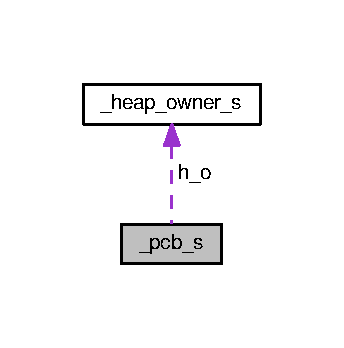
\includegraphics[width=165pt]{struct__pcb__s__coll__graph}
\end{center}
\end{figure}
\subsection*{Data Fields}
\begin{DoxyCompactItemize}
\item 
unsigned long {\bfseries num\+\_\+threads}\hypertarget{struct__pcb__s_a9c8ec4e7d19de58186e633e1c9a4010f}{}\label{struct__pcb__s_a9c8ec4e7d19de58186e633e1c9a4010f}

\item 
void $\ast$ {\bfseries text}\hypertarget{struct__pcb__s_ab704b53133f65b7768f5426fa4529abd}{}\label{struct__pcb__s_ab704b53133f65b7768f5426fa4529abd}

\item 
void $\ast$ {\bfseries data}\hypertarget{struct__pcb__s_a98d408faff3e9592966cee3123937713}{}\label{struct__pcb__s_a98d408faff3e9592966cee3123937713}

\item 
\hyperlink{struct__heap__owner__s}{heap\+\_\+owner\+\_\+t} {\bfseries h\+\_\+o}\hypertarget{struct__pcb__s_af8fff6a773525627aec59f37144dd950}{}\label{struct__pcb__s_af8fff6a773525627aec59f37144dd950}

\end{DoxyCompactItemize}


The documentation for this struct was generated from the following file\+:\begin{DoxyCompactItemize}
\item 
inc/\hyperlink{OS_8h}{O\+S.\+h}\end{DoxyCompactItemize}

\hypertarget{struct__tcb__s}{}\section{\+\_\+tcb\+\_\+s Struct Reference}
\label{struct__tcb__s}\index{\+\_\+tcb\+\_\+s@{\+\_\+tcb\+\_\+s}}


Collaboration diagram for \+\_\+tcb\+\_\+s\+:\nopagebreak
\begin{figure}[H]
\begin{center}
\leavevmode
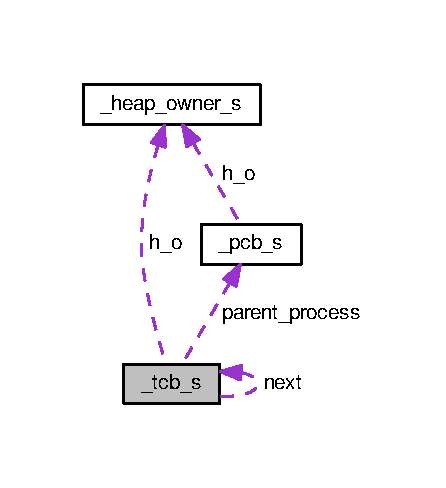
\includegraphics[width=214pt]{struct__tcb__s__coll__graph}
\end{center}
\end{figure}
\subsection*{Data Fields}
\begin{DoxyCompactItemize}
\item 
long $\ast$ {\bfseries sp}\hypertarget{struct__tcb__s_a13f117347df648dbca66e6cbb97a4e0f}{}\label{struct__tcb__s_a13f117347df648dbca66e6cbb97a4e0f}

\item 
struct \hyperlink{struct__tcb__s}{\+\_\+tcb\+\_\+s} $\ast$ {\bfseries next}\hypertarget{struct__tcb__s_af53c260a7b65e7244f809cda9ebb835f}{}\label{struct__tcb__s_af53c260a7b65e7244f809cda9ebb835f}

\item 
uint32\+\_\+t {\bfseries wake\+\_\+time}\hypertarget{struct__tcb__s_a442099ddd859c3f33981828aeef085fe}{}\label{struct__tcb__s_a442099ddd859c3f33981828aeef085fe}

\item 
unsigned long {\bfseries id}\hypertarget{struct__tcb__s_a48e677e5c96cf412d20854802271b9b4}{}\label{struct__tcb__s_a48e677e5c96cf412d20854802271b9b4}

\item 
uint8\+\_\+t {\bfseries priority}\hypertarget{struct__tcb__s_a319151d52db9a3fb0b3c018bce9fcb4a}{}\label{struct__tcb__s_a319151d52db9a3fb0b3c018bce9fcb4a}

\item 
char $\ast$ {\bfseries task\+\_\+name}\hypertarget{struct__tcb__s_a66241e192445da72f98da4e2d1359d5a}{}\label{struct__tcb__s_a66241e192445da72f98da4e2d1359d5a}

\item 
\hyperlink{struct__pcb__s}{pcb\+\_\+t} $\ast$ {\bfseries parent\+\_\+process}\hypertarget{struct__tcb__s_a95f1ceb9227ec81f5fee8d419e38f6f5}{}\label{struct__tcb__s_a95f1ceb9227ec81f5fee8d419e38f6f5}

\item 
long $\ast$ {\bfseries stack\+\_\+base}\hypertarget{struct__tcb__s_a974ef07841ffeb40d1557f239d48c42f}{}\label{struct__tcb__s_a974ef07841ffeb40d1557f239d48c42f}

\item 
\hyperlink{struct__heap__owner__s}{heap\+\_\+owner\+\_\+t} {\bfseries h\+\_\+o}\hypertarget{struct__tcb__s_a3ff5fee4d259b1e8770c961ae8badf6e}{}\label{struct__tcb__s_a3ff5fee4d259b1e8770c961ae8badf6e}

\end{DoxyCompactItemize}


The documentation for this struct was generated from the following file\+:\begin{DoxyCompactItemize}
\item 
inc/\hyperlink{OS_8h}{O\+S.\+h}\end{DoxyCompactItemize}

\input{structDIR}
\input{structElf32__Dyn}
\input{structElf32__Ehdr}
\input{structElf32__Phdr}
\input{structElf32__Rel}
\input{structElf32__Rela}
\input{structElf32__Shdr}
\input{structElf32__Sym}
\input{structELFEnv__t}
\input{structELFSymbol__t}
\input{structevent__t}
\input{structFATFS}
\input{structFIL}
\input{structFILINFO}
\input{structheap__stats}
\hypertarget{structSema4}{}\section{Sema4 Struct Reference}
\label{structSema4}\index{Sema4@{Sema4}}


Collaboration diagram for Sema4\+:\nopagebreak
\begin{figure}[H]
\begin{center}
\leavevmode
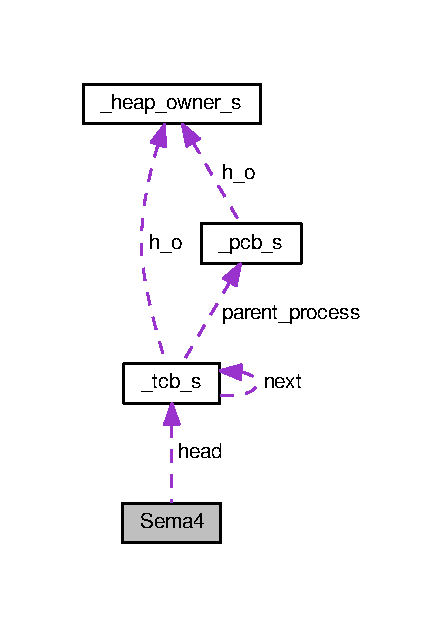
\includegraphics[width=214pt]{structSema4__coll__graph}
\end{center}
\end{figure}
\subsection*{Data Fields}
\begin{DoxyCompactItemize}
\item 
long {\bfseries Value}\hypertarget{structSema4_a98b1e5b4f3a76692bb37db553c22e8b0}{}\label{structSema4_a98b1e5b4f3a76692bb37db553c22e8b0}

\item 
struct \hyperlink{struct__tcb__s}{\+\_\+tcb\+\_\+s} $\ast$ {\bfseries head}\hypertarget{structSema4_a03d774cbfedb9d522f31ded4c10d5668}{}\label{structSema4_a03d774cbfedb9d522f31ded4c10d5668}

\end{DoxyCompactItemize}


The documentation for this struct was generated from the following file\+:\begin{DoxyCompactItemize}
\item 
inc/\hyperlink{OS_8h}{O\+S.\+h}\end{DoxyCompactItemize}

\hypertarget{structtCANBitClkParms}{}\section{t\+C\+A\+N\+Bit\+Clk\+Parms Struct Reference}
\label{structtCANBitClkParms}\index{t\+C\+A\+N\+Bit\+Clk\+Parms@{t\+C\+A\+N\+Bit\+Clk\+Parms}}


{\ttfamily \#include $<$can.\+h$>$}

\subsection*{Data Fields}
\begin{DoxyCompactItemize}
\item 
unsigned int \hyperlink{structtCANBitClkParms_aa99151a686e0a3725b0fd84810ab6d12}{u\+Sync\+Prop\+Phase1\+Seg}
\item 
unsigned int \hyperlink{structtCANBitClkParms_ad95f806349e583b53aaa912f0fada94d}{u\+Phase2\+Seg}
\item 
unsigned int \hyperlink{structtCANBitClkParms_af7d91d76a38a5fe4a2b814bb54db1348}{u\+S\+JW}
\item 
unsigned int \hyperlink{structtCANBitClkParms_a2d5f2674b68dfc7f3c47b6113951e41e}{u\+Quantum\+Prescaler}
\end{DoxyCompactItemize}


\subsection{Detailed Description}
This structure is used for encapsulating the values associated with setting up the bit timing for a C\+AN controller. The structure is used when calling the C\+A\+N\+Get\+Bit\+Timing and C\+A\+N\+Set\+Bit\+Timing functions. 

\subsection{Field Documentation}
\index{t\+C\+A\+N\+Bit\+Clk\+Parms@{t\+C\+A\+N\+Bit\+Clk\+Parms}!u\+Phase2\+Seg@{u\+Phase2\+Seg}}
\index{u\+Phase2\+Seg@{u\+Phase2\+Seg}!t\+C\+A\+N\+Bit\+Clk\+Parms@{t\+C\+A\+N\+Bit\+Clk\+Parms}}
\subsubsection[{\texorpdfstring{u\+Phase2\+Seg}{uPhase2Seg}}]{\setlength{\rightskip}{0pt plus 5cm}unsigned int t\+C\+A\+N\+Bit\+Clk\+Parms\+::u\+Phase2\+Seg}\hypertarget{structtCANBitClkParms_ad95f806349e583b53aaa912f0fada94d}{}\label{structtCANBitClkParms_ad95f806349e583b53aaa912f0fada94d}
This value holds the Phase Buffer 2 segment in time quanta. The valid values for this setting range from 1 to 8. \index{t\+C\+A\+N\+Bit\+Clk\+Parms@{t\+C\+A\+N\+Bit\+Clk\+Parms}!u\+Quantum\+Prescaler@{u\+Quantum\+Prescaler}}
\index{u\+Quantum\+Prescaler@{u\+Quantum\+Prescaler}!t\+C\+A\+N\+Bit\+Clk\+Parms@{t\+C\+A\+N\+Bit\+Clk\+Parms}}
\subsubsection[{\texorpdfstring{u\+Quantum\+Prescaler}{uQuantumPrescaler}}]{\setlength{\rightskip}{0pt plus 5cm}unsigned int t\+C\+A\+N\+Bit\+Clk\+Parms\+::u\+Quantum\+Prescaler}\hypertarget{structtCANBitClkParms_a2d5f2674b68dfc7f3c47b6113951e41e}{}\label{structtCANBitClkParms_a2d5f2674b68dfc7f3c47b6113951e41e}
This value holds the C\+A\+N\+\_\+\+C\+LK divider used to determine time quanta. The valid values for this setting range from 1 to 1023. \index{t\+C\+A\+N\+Bit\+Clk\+Parms@{t\+C\+A\+N\+Bit\+Clk\+Parms}!u\+S\+JW@{u\+S\+JW}}
\index{u\+S\+JW@{u\+S\+JW}!t\+C\+A\+N\+Bit\+Clk\+Parms@{t\+C\+A\+N\+Bit\+Clk\+Parms}}
\subsubsection[{\texorpdfstring{u\+S\+JW}{uSJW}}]{\setlength{\rightskip}{0pt plus 5cm}unsigned int t\+C\+A\+N\+Bit\+Clk\+Parms\+::u\+S\+JW}\hypertarget{structtCANBitClkParms_af7d91d76a38a5fe4a2b814bb54db1348}{}\label{structtCANBitClkParms_af7d91d76a38a5fe4a2b814bb54db1348}
This value holds the Resynchronization Jump Width in time quanta. The valid values for this setting range from 1 to 4. \index{t\+C\+A\+N\+Bit\+Clk\+Parms@{t\+C\+A\+N\+Bit\+Clk\+Parms}!u\+Sync\+Prop\+Phase1\+Seg@{u\+Sync\+Prop\+Phase1\+Seg}}
\index{u\+Sync\+Prop\+Phase1\+Seg@{u\+Sync\+Prop\+Phase1\+Seg}!t\+C\+A\+N\+Bit\+Clk\+Parms@{t\+C\+A\+N\+Bit\+Clk\+Parms}}
\subsubsection[{\texorpdfstring{u\+Sync\+Prop\+Phase1\+Seg}{uSyncPropPhase1Seg}}]{\setlength{\rightskip}{0pt plus 5cm}unsigned int t\+C\+A\+N\+Bit\+Clk\+Parms\+::u\+Sync\+Prop\+Phase1\+Seg}\hypertarget{structtCANBitClkParms_aa99151a686e0a3725b0fd84810ab6d12}{}\label{structtCANBitClkParms_aa99151a686e0a3725b0fd84810ab6d12}
This value holds the sum of the Synchronization, Propagation, and Phase Buffer 1 segments, measured in time quanta. The valid values for this setting range from 2 to 16. 

The documentation for this struct was generated from the following file\+:\begin{DoxyCompactItemize}
\item 
inc/can.\+h\end{DoxyCompactItemize}

\hypertarget{structtCANMsgObject}{}\section{t\+C\+A\+N\+Msg\+Object Struct Reference}
\label{structtCANMsgObject}\index{t\+C\+A\+N\+Msg\+Object@{t\+C\+A\+N\+Msg\+Object}}


{\ttfamily \#include $<$can.\+h$>$}

\subsection*{Data Fields}
\begin{DoxyCompactItemize}
\item 
uint32\+\_\+t \hyperlink{structtCANMsgObject_a663d0cdd6893cd3ee998795dd0620dfd}{ul\+Msg\+ID}\hypertarget{structtCANMsgObject_a663d0cdd6893cd3ee998795dd0620dfd}{}\label{structtCANMsgObject_a663d0cdd6893cd3ee998795dd0620dfd}

\begin{DoxyCompactList}\small\item\em The C\+AN message identifier used for 11 or 29 bit identifiers. \end{DoxyCompactList}\item 
uint32\+\_\+t \hyperlink{structtCANMsgObject_a99a0c309158bfe53401884a66711e80c}{ul\+Msg\+I\+D\+Mask}\hypertarget{structtCANMsgObject_a99a0c309158bfe53401884a66711e80c}{}\label{structtCANMsgObject_a99a0c309158bfe53401884a66711e80c}

\begin{DoxyCompactList}\small\item\em The message identifier mask used when identifier filtering is enabled. \end{DoxyCompactList}\item 
uint32\+\_\+t \hyperlink{structtCANMsgObject_a23801a4be509591978e7b4f9bcafe124}{ul\+Flags}
\item 
uint32\+\_\+t \hyperlink{structtCANMsgObject_a5364beed437bfdfa7c536ab5b3417ea9}{ul\+Msg\+Len}\hypertarget{structtCANMsgObject_a5364beed437bfdfa7c536ab5b3417ea9}{}\label{structtCANMsgObject_a5364beed437bfdfa7c536ab5b3417ea9}

\begin{DoxyCompactList}\small\item\em This value is the number of bytes of data in the message object. \end{DoxyCompactList}\item 
uint8\+\_\+t $\ast$ \hyperlink{structtCANMsgObject_a2f2a9f1ed9b01b6a2caf2256ec938a1b}{puc\+Msg\+Data}\hypertarget{structtCANMsgObject_a2f2a9f1ed9b01b6a2caf2256ec938a1b}{}\label{structtCANMsgObject_a2f2a9f1ed9b01b6a2caf2256ec938a1b}

\begin{DoxyCompactList}\small\item\em This is a pointer to the message object\textquotesingle{}s data. \end{DoxyCompactList}\end{DoxyCompactItemize}


\subsection{Detailed Description}
The structure used for encapsulating all the items associated with a C\+AN message object in the C\+AN controller. 

\subsection{Field Documentation}
\index{t\+C\+A\+N\+Msg\+Object@{t\+C\+A\+N\+Msg\+Object}!ul\+Flags@{ul\+Flags}}
\index{ul\+Flags@{ul\+Flags}!t\+C\+A\+N\+Msg\+Object@{t\+C\+A\+N\+Msg\+Object}}
\subsubsection[{\texorpdfstring{ul\+Flags}{ulFlags}}]{\setlength{\rightskip}{0pt plus 5cm}uint32\+\_\+t t\+C\+A\+N\+Msg\+Object\+::ul\+Flags}\hypertarget{structtCANMsgObject_a23801a4be509591978e7b4f9bcafe124}{}\label{structtCANMsgObject_a23801a4be509591978e7b4f9bcafe124}
This value holds various status flags and settings specified by t\+C\+A\+N\+Obj\+Flags. 

The documentation for this struct was generated from the following file\+:\begin{DoxyCompactItemize}
\item 
inc/can.\+h\end{DoxyCompactItemize}

\chapter{File Documentation}
\hypertarget{ADC_8h}{}\section{inc/\+A\+DC.h File Reference}
\label{ADC_8h}\index{inc/\+A\+D\+C.\+h@{inc/\+A\+D\+C.\+h}}


A\+DC driver for the T\+M4\+C123G. Provides interfaces for collecting single samples or a series at a given sampling frequency. Does not allow for sampling of more than one channel at any given time. Timer 2 is reserved for this driver.  


{\ttfamily \#include $<$stdint.\+h$>$}\\*
Include dependency graph for A\+D\+C.\+h\+:\nopagebreak
\begin{figure}[H]
\begin{center}
\leavevmode
\includegraphics[width=142pt]{ADC_8h__incl}
\end{center}
\end{figure}
\subsection*{Functions}
\begin{DoxyCompactItemize}
\item 
int \hyperlink{ADC_8h_af9d370fc407dee15db32335255f6cf74}{A\+D\+C\+\_\+\+Init} (uint32\+\_\+t channel\+Num)
\begin{DoxyCompactList}\small\item\em Configure an A\+DC channel for continuous sampling. Retrieve measurements from this channel with \hyperlink{ADC_8h_a25269c67b0ba9dd124734e05ffb38493}{A\+D\+C\+\_\+\+In()}. \end{DoxyCompactList}\item 
uint16\+\_\+t \hyperlink{ADC_8h_a25269c67b0ba9dd124734e05ffb38493}{A\+D\+C\+\_\+\+In} (void)
\begin{DoxyCompactList}\small\item\em Returns the most recent sample collected by the channel configured in A\+D\+C\+\_\+\+Init(...) \end{DoxyCompactList}\item 
int \hyperlink{ADC_8h_a262f417393c62f81b4a37b3019b32095}{A\+D\+C\+\_\+\+Collect} (uint32\+\_\+t channel\+Num, uint32\+\_\+t fs, void($\ast$handler)(unsigned long))
\begin{DoxyCompactList}\small\item\em Kick off collection of a sequence of samples to be passed to a user-\/provided handler. The A\+DC and Timer will be configured to collect samples at frequency fs. \end{DoxyCompactList}\end{DoxyCompactItemize}


\subsection{Detailed Description}
A\+DC driver for the T\+M4\+C123G. Provides interfaces for collecting single samples or a series at a given sampling frequency. Does not allow for sampling of more than one channel at any given time. Timer 2 is reserved for this driver. 

\begin{DoxyAuthor}{Author}
Riley Wood and Jeageun Jung 
\end{DoxyAuthor}


\subsection{Function Documentation}
\index{A\+D\+C.\+h@{A\+D\+C.\+h}!A\+D\+C\+\_\+\+Collect@{A\+D\+C\+\_\+\+Collect}}
\index{A\+D\+C\+\_\+\+Collect@{A\+D\+C\+\_\+\+Collect}!A\+D\+C.\+h@{A\+D\+C.\+h}}
\subsubsection[{\texorpdfstring{A\+D\+C\+\_\+\+Collect(uint32\+\_\+t channel\+Num, uint32\+\_\+t fs, void($\ast$handler)(unsigned long))}{ADC_Collect(uint32_t channelNum, uint32_t fs, void(*handler)(unsigned long))}}]{\setlength{\rightskip}{0pt plus 5cm}int A\+D\+C\+\_\+\+Collect (
\begin{DoxyParamCaption}
\item[{uint32\+\_\+t}]{channel\+Num, }
\item[{uint32\+\_\+t}]{fs, }
\item[{void($\ast$)(unsigned long)}]{handler}
\end{DoxyParamCaption}
)}\hypertarget{ADC_8h_a262f417393c62f81b4a37b3019b32095}{}\label{ADC_8h_a262f417393c62f81b4a37b3019b32095}


Kick off collection of a sequence of samples to be passed to a user-\/provided handler. The A\+DC and Timer will be configured to collect samples at frequency fs. 


\begin{DoxyParams}{Parameters}
{\em channel\+Num} & A\+DC channel to sample \\
\hline
{\em fs} & Sampling frequency \\
\hline
{\em handler} & Function which will be passed each sample as it is collected. \\
\hline
\end{DoxyParams}
\begin{DoxyReturn}{Returns}
int 0 on success, -\/1 on failure. 
\end{DoxyReturn}
\index{A\+D\+C.\+h@{A\+D\+C.\+h}!A\+D\+C\+\_\+\+In@{A\+D\+C\+\_\+\+In}}
\index{A\+D\+C\+\_\+\+In@{A\+D\+C\+\_\+\+In}!A\+D\+C.\+h@{A\+D\+C.\+h}}
\subsubsection[{\texorpdfstring{A\+D\+C\+\_\+\+In(void)}{ADC_In(void)}}]{\setlength{\rightskip}{0pt plus 5cm}uint16\+\_\+t A\+D\+C\+\_\+\+In (
\begin{DoxyParamCaption}
\item[{void}]{}
\end{DoxyParamCaption}
)}\hypertarget{ADC_8h_a25269c67b0ba9dd124734e05ffb38493}{}\label{ADC_8h_a25269c67b0ba9dd124734e05ffb38493}


Returns the most recent sample collected by the channel configured in A\+D\+C\+\_\+\+Init(...) 

This function uses busy-\/wait for the A\+DC sampling to be done

\begin{DoxyReturn}{Returns}
uint16\+\_\+t The conversion result 
\end{DoxyReturn}
\index{A\+D\+C.\+h@{A\+D\+C.\+h}!A\+D\+C\+\_\+\+Init@{A\+D\+C\+\_\+\+Init}}
\index{A\+D\+C\+\_\+\+Init@{A\+D\+C\+\_\+\+Init}!A\+D\+C.\+h@{A\+D\+C.\+h}}
\subsubsection[{\texorpdfstring{A\+D\+C\+\_\+\+Init(uint32\+\_\+t channel\+Num)}{ADC_Init(uint32_t channelNum)}}]{\setlength{\rightskip}{0pt plus 5cm}int A\+D\+C\+\_\+\+Init (
\begin{DoxyParamCaption}
\item[{uint32\+\_\+t}]{channel\+Num}
\end{DoxyParamCaption}
)}\hypertarget{ADC_8h_af9d370fc407dee15db32335255f6cf74}{}\label{ADC_8h_af9d370fc407dee15db32335255f6cf74}


Configure an A\+DC channel for continuous sampling. Retrieve measurements from this channel with \hyperlink{ADC_8h_a25269c67b0ba9dd124734e05ffb38493}{A\+D\+C\+\_\+\+In()}. 


\begin{DoxyParams}{Parameters}
{\em channel\+Num} & The channel to set up \\
\hline
\end{DoxyParams}
\begin{DoxyReturn}{Returns}
int 0 on success, -\/1 on failure. 
\end{DoxyReturn}

\input{diskio_8h}
\input{ff_8h}
\hypertarget{heap_8h}{}\section{inc/heap.h File Reference}
\label{heap_8h}\index{inc/heap.\+h@{inc/heap.\+h}}


Implements memory heap for dynamic memory allocation. Follows standard malloc/calloc/realloc/free interface for allocating/unallocating memory. modified 8/31/08 Jonathan Valvano for style modified 12/16/11 Jonathan Valvano for 32-\/bit machine modified August 10, 2014 for C99 syntax This example accompanies the book \char`\"{}\+Embedded Systems\+: Real Time Operating Systems for A\+R\+M Cortex M Microcontrollers\char`\"{}, I\+S\+BN\+: 978-\/1466468863, Jonathan Valvano, copyright (c) 2014 Implementation Notes\+: This is a Knuth Heap. Each block has a header and a trailer, which I shall call the meta-\/sections. The meta-\/sections are each a single int32\+\_\+t that tells how many int32\+\_\+ts/words can be stored between the header and trailer. If the block is used, the meta-\/sections record the room as a positive number. If the block is unused, the meta-\/sections record the room as a negative number. Copyright 2014 by Jonathan W. Valvano, \href{mailto:valvano@mail.utexas.edu}{\tt valvano@mail.\+utexas.\+edu} You may use, edit, run or distribute this file as long as the above copyright notice remains T\+H\+IS S\+O\+F\+T\+W\+A\+RE IS P\+R\+O\+V\+I\+D\+ED \char`\"{}\+A\+S I\+S\char`\"{}. NO W\+A\+R\+R\+A\+N\+T\+I\+ES, W\+H\+E\+T\+H\+ER E\+X\+P\+R\+E\+SS, I\+M\+P\+L\+I\+ED OR S\+T\+A\+T\+U\+T\+O\+RY, I\+N\+C\+L\+U\+D\+I\+NG, B\+UT N\+OT L\+I\+M\+I\+T\+ED TO, I\+M\+P\+L\+I\+ED W\+A\+R\+R\+A\+N\+T\+I\+ES OF M\+E\+R\+C\+H\+A\+N\+T\+A\+B\+I\+L\+I\+TY A\+ND F\+I\+T\+N\+E\+SS F\+OR A P\+A\+R\+T\+I\+C\+U\+L\+AR P\+U\+R\+P\+O\+SE A\+P\+P\+LY TO T\+H\+IS S\+O\+F\+T\+W\+A\+RE. V\+A\+L\+V\+A\+NO S\+H\+A\+LL N\+OT, IN A\+NY C\+I\+R\+C\+U\+M\+S\+T\+A\+N\+C\+ES, BE L\+I\+A\+B\+LE F\+OR S\+P\+E\+C\+I\+AL, I\+N\+C\+I\+D\+E\+N\+T\+AL, OR C\+O\+N\+S\+E\+Q\+U\+E\+N\+T\+I\+AL D\+A\+M\+A\+G\+ES, F\+OR A\+NY R\+E\+A\+S\+ON W\+H\+A\+T\+S\+O\+E\+V\+ER. For more information about my classes, my research, and my books, see \href{http://users.ece.utexas.edu/~valvano/}{\tt http\+://users.\+ece.\+utexas.\+edu/$\sim$valvano/}.  


This graph shows which files directly or indirectly include this file\+:\nopagebreak
\begin{figure}[H]
\begin{center}
\leavevmode
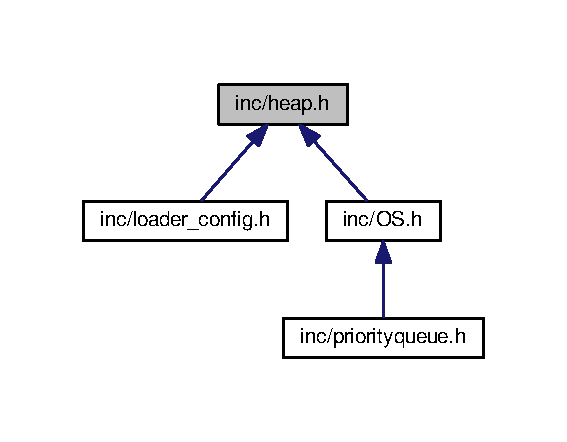
\includegraphics[width=272pt]{heap_8h__dep__incl}
\end{center}
\end{figure}
\subsection*{Data Structures}
\begin{DoxyCompactItemize}
\item 
struct \hyperlink{struct__heap__owner__s}{\+\_\+heap\+\_\+owner\+\_\+s}
\item 
struct \hyperlink{structheap__stats}{heap\+\_\+stats}
\end{DoxyCompactItemize}
\subsection*{Macros}
\begin{DoxyCompactItemize}
\item 
\#define {\bfseries H\+E\+A\+P\+\_\+\+S\+I\+Z\+E\+\_\+\+B\+Y\+T\+ES}~(16384)\hypertarget{heap_8h_af2910747af799b24cfaa2ab32861f592}{}\label{heap_8h_af2910747af799b24cfaa2ab32861f592}

\item 
\#define {\bfseries H\+E\+A\+P\+\_\+\+S\+I\+Z\+E\+\_\+\+W\+O\+R\+DS}~(H\+E\+A\+P\+\_\+\+S\+I\+Z\+E\+\_\+\+B\+Y\+T\+ES / sizeof(int32\+\_\+t))\hypertarget{heap_8h_a08198ef17b67d091f9eb38c544cb4680}{}\label{heap_8h_a08198ef17b67d091f9eb38c544cb4680}

\item 
\#define {\bfseries H\+E\+A\+P\+\_\+\+OK}~0\hypertarget{heap_8h_aa57d61dd0e8d07dce08f6be38001a5ff}{}\label{heap_8h_aa57d61dd0e8d07dce08f6be38001a5ff}

\item 
\#define {\bfseries H\+E\+A\+P\+\_\+\+E\+R\+R\+O\+R\+\_\+\+C\+O\+R\+R\+U\+P\+T\+E\+D\+\_\+\+H\+E\+AP}~1\hypertarget{heap_8h_a4741d1e0f188dbcd4fe46ec0038c59c7}{}\label{heap_8h_a4741d1e0f188dbcd4fe46ec0038c59c7}

\item 
\#define {\bfseries H\+E\+A\+P\+\_\+\+E\+R\+R\+O\+R\+\_\+\+P\+O\+I\+N\+T\+E\+R\+\_\+\+O\+U\+T\+\_\+\+O\+F\+\_\+\+R\+A\+N\+GE}~2\hypertarget{heap_8h_a5400f746fb9c8efb71156c51f766b22e}{}\label{heap_8h_a5400f746fb9c8efb71156c51f766b22e}

\item 
\#define \hyperlink{heap_8h_a99c93bda9ddc931ef53738d1f4961d58}{Heap\+\_\+\+Malloc}(desired\+Bytes)~\+\_\+\+\_\+\+Heap\+\_\+\+Malloc(desired\+Bytes, \&cur\+\_\+tcb-\/$>$h\+\_\+o)
\begin{DoxyCompactList}\small\item\em Allocate memory, data not initialized. \end{DoxyCompactList}\end{DoxyCompactItemize}
\subsection*{Typedefs}
\begin{DoxyCompactItemize}
\item 
typedef struct \hyperlink{struct__heap__owner__s}{\+\_\+heap\+\_\+owner\+\_\+s} {\bfseries heap\+\_\+owner\+\_\+t}\hypertarget{heap_8h_a3df85fc1dfba9c3bdc8f325c84d70e3d}{}\label{heap_8h_a3df85fc1dfba9c3bdc8f325c84d70e3d}

\item 
typedef struct \hyperlink{structheap__stats}{heap\+\_\+stats} {\bfseries heap\+\_\+stats\+\_\+t}\hypertarget{heap_8h_a286400a036f6f2dc8a3ddca156720932}{}\label{heap_8h_a286400a036f6f2dc8a3ddca156720932}

\end{DoxyCompactItemize}
\subsection*{Functions}
\begin{DoxyCompactItemize}
\item 
int32\+\_\+t \hyperlink{heap_8h_a927f9f9522b87a3ccaee6c68efbf2081}{Heap\+\_\+\+Init} (void)
\begin{DoxyCompactList}\small\item\em Initialize the Heap notes\+: Initializes/resets the heap to a clean state where no memory is allocated. \end{DoxyCompactList}\item 
void $\ast$ {\bfseries O\+S\+\_\+\+S\+V\+C\+\_\+\+Heap\+\_\+\+Malloc} (int32\+\_\+t desired\+Bytes)\hypertarget{heap_8h_a6866ead55d5e2091e5ac1e4c4b1f231f}{}\label{heap_8h_a6866ead55d5e2091e5ac1e4c4b1f231f}

\item 
void $\ast$ {\bfseries \+\_\+\+\_\+\+Heap\+\_\+\+Malloc} (int32\+\_\+t desired\+Bytes, \hyperlink{struct__heap__owner__s}{heap\+\_\+owner\+\_\+t} $\ast$owner)\hypertarget{heap_8h_a44f034fef9e00ee50b74a0cfd9f2dd22}{}\label{heap_8h_a44f034fef9e00ee50b74a0cfd9f2dd22}

\item 
void $\ast$ \hyperlink{heap_8h_a2844e924abca6846ed9407e57ed828ab}{Heap\+\_\+\+Calloc} (int32\+\_\+t desired\+Bytes)
\begin{DoxyCompactList}\small\item\em Allocate memory, data are initialized to 0 notes\+: the allocated memory block will be zeroed out. \end{DoxyCompactList}\item 
void $\ast$ \hyperlink{heap_8h_af02282279b1745e0e1485c5bc7d19098}{Heap\+\_\+\+Realloc} (void $\ast$old\+Block, int32\+\_\+t desired\+Bytes)
\begin{DoxyCompactList}\small\item\em Reallocate buffer to a new size notes\+: the given block will be unallocated after its contents are copied to the new block. \end{DoxyCompactList}\item 
int32\+\_\+t \hyperlink{heap_8h_a92c7ac360bf78ce4a7498a44b345c8c1}{\+\_\+\+\_\+\+Heap\+\_\+\+Change\+Owner} (void $\ast$pointer, \hyperlink{struct__heap__owner__s}{heap\+\_\+owner\+\_\+t} $\ast$new\+\_\+owner)
\begin{DoxyCompactList}\small\item\em Change ownership of block to the given task. This is only meant to be used by the OS for task management in processes. \end{DoxyCompactList}\item 
int32\+\_\+t \hyperlink{heap_8h_a0c2946e20398909f89ebf1bc344b9f60}{Heap\+\_\+\+Free} (void $\ast$pointer)
\begin{DoxyCompactList}\small\item\em return a block to the heap \end{DoxyCompactList}\item 
int32\+\_\+t {\bfseries O\+S\+\_\+\+S\+V\+C\+\_\+\+Heap\+\_\+\+Free} (void $\ast$pointer)\hypertarget{heap_8h_ae58fc24993d48bb6a1775b016d5b9e95}{}\label{heap_8h_ae58fc24993d48bb6a1775b016d5b9e95}

\item 
int32\+\_\+t \hyperlink{heap_8h_a5c8d75b021d5e6edab5c8e0164224e3e}{Heap\+\_\+\+Test} (void)
\begin{DoxyCompactList}\small\item\em Test the heap. \end{DoxyCompactList}\item 
\hyperlink{structheap__stats}{heap\+\_\+stats\+\_\+t} \hyperlink{heap_8h_a21054e474258ea882ed5765cabaa7c3b}{Heap\+\_\+\+Stats} (void)
\begin{DoxyCompactList}\small\item\em return the current status of the heap \end{DoxyCompactList}\end{DoxyCompactItemize}


\subsection{Detailed Description}
Implements memory heap for dynamic memory allocation. Follows standard malloc/calloc/realloc/free interface for allocating/unallocating memory. modified 8/31/08 Jonathan Valvano for style modified 12/16/11 Jonathan Valvano for 32-\/bit machine modified August 10, 2014 for C99 syntax This example accompanies the book \char`\"{}\+Embedded Systems\+: Real Time Operating Systems for A\+R\+M Cortex M Microcontrollers\char`\"{}, I\+S\+BN\+: 978-\/1466468863, Jonathan Valvano, copyright (c) 2014 Implementation Notes\+: This is a Knuth Heap. Each block has a header and a trailer, which I shall call the meta-\/sections. The meta-\/sections are each a single int32\+\_\+t that tells how many int32\+\_\+ts/words can be stored between the header and trailer. If the block is used, the meta-\/sections record the room as a positive number. If the block is unused, the meta-\/sections record the room as a negative number. Copyright 2014 by Jonathan W. Valvano, \href{mailto:valvano@mail.utexas.edu}{\tt valvano@mail.\+utexas.\+edu} You may use, edit, run or distribute this file as long as the above copyright notice remains T\+H\+IS S\+O\+F\+T\+W\+A\+RE IS P\+R\+O\+V\+I\+D\+ED \char`\"{}\+A\+S I\+S\char`\"{}. NO W\+A\+R\+R\+A\+N\+T\+I\+ES, W\+H\+E\+T\+H\+ER E\+X\+P\+R\+E\+SS, I\+M\+P\+L\+I\+ED OR S\+T\+A\+T\+U\+T\+O\+RY, I\+N\+C\+L\+U\+D\+I\+NG, B\+UT N\+OT L\+I\+M\+I\+T\+ED TO, I\+M\+P\+L\+I\+ED W\+A\+R\+R\+A\+N\+T\+I\+ES OF M\+E\+R\+C\+H\+A\+N\+T\+A\+B\+I\+L\+I\+TY A\+ND F\+I\+T\+N\+E\+SS F\+OR A P\+A\+R\+T\+I\+C\+U\+L\+AR P\+U\+R\+P\+O\+SE A\+P\+P\+LY TO T\+H\+IS S\+O\+F\+T\+W\+A\+RE. V\+A\+L\+V\+A\+NO S\+H\+A\+LL N\+OT, IN A\+NY C\+I\+R\+C\+U\+M\+S\+T\+A\+N\+C\+ES, BE L\+I\+A\+B\+LE F\+OR S\+P\+E\+C\+I\+AL, I\+N\+C\+I\+D\+E\+N\+T\+AL, OR C\+O\+N\+S\+E\+Q\+U\+E\+N\+T\+I\+AL D\+A\+M\+A\+G\+ES, F\+OR A\+NY R\+E\+A\+S\+ON W\+H\+A\+T\+S\+O\+E\+V\+ER. For more information about my classes, my research, and my books, see \href{http://users.ece.utexas.edu/~valvano/}{\tt http\+://users.\+ece.\+utexas.\+edu/$\sim$valvano/}. 

\begin{DoxyAuthor}{Author}
Jacob Egner 
\end{DoxyAuthor}
\begin{DoxyDate}{Date}
2008-\/07-\/31 
\end{DoxyDate}


\subsection{Macro Definition Documentation}
\index{heap.\+h@{heap.\+h}!Heap\+\_\+\+Malloc@{Heap\+\_\+\+Malloc}}
\index{Heap\+\_\+\+Malloc@{Heap\+\_\+\+Malloc}!heap.\+h@{heap.\+h}}
\subsubsection[{\texorpdfstring{Heap\+\_\+\+Malloc}{Heap_Malloc}}]{\setlength{\rightskip}{0pt plus 5cm}\#define Heap\+\_\+\+Malloc(
\begin{DoxyParamCaption}
\item[{}]{desired\+Bytes}
\end{DoxyParamCaption}
)~\+\_\+\+\_\+\+Heap\+\_\+\+Malloc(desired\+Bytes, \&cur\+\_\+tcb-\/$>$h\+\_\+o)}\hypertarget{heap_8h_a99c93bda9ddc931ef53738d1f4961d58}{}\label{heap_8h_a99c93bda9ddc931ef53738d1f4961d58}


Allocate memory, data not initialized. 


\begin{DoxyParams}{Parameters}
{\em desired\+Bytes} & desired number of bytes to allocate\\
\hline
\end{DoxyParams}
\begin{DoxyReturn}{Returns}
void$\ast$ pointing to the allocated memory or will return N\+U\+LL if there isn\textquotesingle{}t sufficient space to satisfy allocation request 
\end{DoxyReturn}


\subsection{Function Documentation}
\index{heap.\+h@{heap.\+h}!\+\_\+\+\_\+\+Heap\+\_\+\+Change\+Owner@{\+\_\+\+\_\+\+Heap\+\_\+\+Change\+Owner}}
\index{\+\_\+\+\_\+\+Heap\+\_\+\+Change\+Owner@{\+\_\+\+\_\+\+Heap\+\_\+\+Change\+Owner}!heap.\+h@{heap.\+h}}
\subsubsection[{\texorpdfstring{\+\_\+\+\_\+\+Heap\+\_\+\+Change\+Owner(void $\ast$pointer, heap\+\_\+owner\+\_\+t $\ast$new\+\_\+owner)}{__Heap_ChangeOwner(void *pointer, heap_owner_t *new_owner)}}]{\setlength{\rightskip}{0pt plus 5cm}int32\+\_\+t \+\_\+\+\_\+\+Heap\+\_\+\+Change\+Owner (
\begin{DoxyParamCaption}
\item[{void $\ast$}]{pointer, }
\item[{{\bf heap\+\_\+owner\+\_\+t} $\ast$}]{new\+\_\+owner}
\end{DoxyParamCaption}
)}\hypertarget{heap_8h_a92c7ac360bf78ce4a7498a44b345c8c1}{}\label{heap_8h_a92c7ac360bf78ce4a7498a44b345c8c1}


Change ownership of block to the given task. This is only meant to be used by the OS for task management in processes. 


\begin{DoxyParams}{Parameters}
{\em pointer} & Pointer to the start of the block in the heap. \\
\hline
{\em new\+\_\+owner} & Task that will own the block after this call exits successfully. \\
\hline
\end{DoxyParams}
\begin{DoxyReturn}{Returns}
int32\+\_\+t H\+E\+A\+P\+\_\+\+OK if everything is ok; H\+E\+A\+P\+\_\+\+E\+R\+R\+O\+R\+\_\+\+P\+O\+I\+N\+T\+E\+R\+\_\+\+O\+U\+T\+\_\+\+O\+F\+\_\+\+R\+A\+N\+GE if pointer points outside the heap; H\+E\+A\+P\+\_\+\+E\+R\+R\+O\+R\+\_\+\+C\+O\+R\+R\+U\+P\+T\+E\+D\+\_\+\+H\+E\+AP if heap has been corrupted or trying to unallocate memory that has already been unallocated; 
\end{DoxyReturn}
\index{heap.\+h@{heap.\+h}!Heap\+\_\+\+Calloc@{Heap\+\_\+\+Calloc}}
\index{Heap\+\_\+\+Calloc@{Heap\+\_\+\+Calloc}!heap.\+h@{heap.\+h}}
\subsubsection[{\texorpdfstring{Heap\+\_\+\+Calloc(int32\+\_\+t desired\+Bytes)}{Heap_Calloc(int32_t desiredBytes)}}]{\setlength{\rightskip}{0pt plus 5cm}void$\ast$ Heap\+\_\+\+Calloc (
\begin{DoxyParamCaption}
\item[{int32\+\_\+t}]{desired\+Bytes}
\end{DoxyParamCaption}
)}\hypertarget{heap_8h_a2844e924abca6846ed9407e57ed828ab}{}\label{heap_8h_a2844e924abca6846ed9407e57ed828ab}


Allocate memory, data are initialized to 0 notes\+: the allocated memory block will be zeroed out. 


\begin{DoxyParams}{Parameters}
{\em desired\+Bytes} & desired number of bytes to allocate\\
\hline
\end{DoxyParams}
\begin{DoxyReturn}{Returns}
void$\ast$ pointing to the allocated memory block or will return N\+U\+LL if there isn\textquotesingle{}t sufficient space to satisfy allocation request 
\end{DoxyReturn}
\index{heap.\+h@{heap.\+h}!Heap\+\_\+\+Free@{Heap\+\_\+\+Free}}
\index{Heap\+\_\+\+Free@{Heap\+\_\+\+Free}!heap.\+h@{heap.\+h}}
\subsubsection[{\texorpdfstring{Heap\+\_\+\+Free(void $\ast$pointer)}{Heap_Free(void *pointer)}}]{\setlength{\rightskip}{0pt plus 5cm}int32\+\_\+t Heap\+\_\+\+Free (
\begin{DoxyParamCaption}
\item[{void $\ast$}]{pointer}
\end{DoxyParamCaption}
)}\hypertarget{heap_8h_a0c2946e20398909f89ebf1bc344b9f60}{}\label{heap_8h_a0c2946e20398909f89ebf1bc344b9f60}


return a block to the heap 


\begin{DoxyParams}{Parameters}
{\em pointer} & the pointer to memory to unallocate\\
\hline
\end{DoxyParams}
\begin{DoxyReturn}{Returns}
H\+E\+A\+P\+\_\+\+OK if everything is ok; H\+E\+A\+P\+\_\+\+E\+R\+R\+O\+R\+\_\+\+P\+O\+I\+N\+T\+E\+R\+\_\+\+O\+U\+T\+\_\+\+O\+F\+\_\+\+R\+A\+N\+GE if pointer points outside the heap; H\+E\+A\+P\+\_\+\+E\+R\+R\+O\+R\+\_\+\+C\+O\+R\+R\+U\+P\+T\+E\+D\+\_\+\+H\+E\+AP if heap has been corrupted or trying to unallocate memory that has already been unallocated; 
\end{DoxyReturn}
\index{heap.\+h@{heap.\+h}!Heap\+\_\+\+Init@{Heap\+\_\+\+Init}}
\index{Heap\+\_\+\+Init@{Heap\+\_\+\+Init}!heap.\+h@{heap.\+h}}
\subsubsection[{\texorpdfstring{Heap\+\_\+\+Init(void)}{Heap_Init(void)}}]{\setlength{\rightskip}{0pt plus 5cm}int32\+\_\+t Heap\+\_\+\+Init (
\begin{DoxyParamCaption}
\item[{void}]{}
\end{DoxyParamCaption}
)}\hypertarget{heap_8h_a927f9f9522b87a3ccaee6c68efbf2081}{}\label{heap_8h_a927f9f9522b87a3ccaee6c68efbf2081}


Initialize the Heap notes\+: Initializes/resets the heap to a clean state where no memory is allocated. 

\begin{DoxyReturn}{Returns}
always H\+E\+A\+P\+\_\+\+OK 
\end{DoxyReturn}
\index{heap.\+h@{heap.\+h}!Heap\+\_\+\+Realloc@{Heap\+\_\+\+Realloc}}
\index{Heap\+\_\+\+Realloc@{Heap\+\_\+\+Realloc}!heap.\+h@{heap.\+h}}
\subsubsection[{\texorpdfstring{Heap\+\_\+\+Realloc(void $\ast$old\+Block, int32\+\_\+t desired\+Bytes)}{Heap_Realloc(void *oldBlock, int32_t desiredBytes)}}]{\setlength{\rightskip}{0pt plus 5cm}void$\ast$ Heap\+\_\+\+Realloc (
\begin{DoxyParamCaption}
\item[{void $\ast$}]{old\+Block, }
\item[{int32\+\_\+t}]{desired\+Bytes}
\end{DoxyParamCaption}
)}\hypertarget{heap_8h_af02282279b1745e0e1485c5bc7d19098}{}\label{heap_8h_af02282279b1745e0e1485c5bc7d19098}


Reallocate buffer to a new size notes\+: the given block will be unallocated after its contents are copied to the new block. 


\begin{DoxyParams}{Parameters}
{\em old\+Block} & pointer to a block\\
\hline
{\em desired\+Bytes} & a desired number of bytes for a new block where the contents of the old block will be copied to\\
\hline
\end{DoxyParams}
\begin{DoxyReturn}{Returns}
void$\ast$ pointing to the new block or will return N\+U\+LL if there is any reason the reallocation can\textquotesingle{}t be completed 
\end{DoxyReturn}
\index{heap.\+h@{heap.\+h}!Heap\+\_\+\+Stats@{Heap\+\_\+\+Stats}}
\index{Heap\+\_\+\+Stats@{Heap\+\_\+\+Stats}!heap.\+h@{heap.\+h}}
\subsubsection[{\texorpdfstring{Heap\+\_\+\+Stats(void)}{Heap_Stats(void)}}]{\setlength{\rightskip}{0pt plus 5cm}{\bf heap\+\_\+stats\+\_\+t} Heap\+\_\+\+Stats (
\begin{DoxyParamCaption}
\item[{void}]{}
\end{DoxyParamCaption}
)}\hypertarget{heap_8h_a21054e474258ea882ed5765cabaa7c3b}{}\label{heap_8h_a21054e474258ea882ed5765cabaa7c3b}


return the current status of the heap 

\begin{DoxyReturn}{Returns}
a heap\+\_\+stats\+\_\+t that describes the current usage of the heap 
\end{DoxyReturn}
\index{heap.\+h@{heap.\+h}!Heap\+\_\+\+Test@{Heap\+\_\+\+Test}}
\index{Heap\+\_\+\+Test@{Heap\+\_\+\+Test}!heap.\+h@{heap.\+h}}
\subsubsection[{\texorpdfstring{Heap\+\_\+\+Test(void)}{Heap_Test(void)}}]{\setlength{\rightskip}{0pt plus 5cm}int32\+\_\+t Heap\+\_\+\+Test (
\begin{DoxyParamCaption}
\item[{void}]{}
\end{DoxyParamCaption}
)}\hypertarget{heap_8h_a5c8d75b021d5e6edab5c8e0164224e3e}{}\label{heap_8h_a5c8d75b021d5e6edab5c8e0164224e3e}


Test the heap. 

\begin{DoxyReturn}{Returns}
validity of the heap -\/ either H\+E\+A\+P\+\_\+\+OK or H\+E\+A\+P\+\_\+\+E\+R\+R\+O\+R\+\_\+\+H\+E\+A\+P\+\_\+\+C\+O\+R\+R\+U\+P\+T\+ED 
\end{DoxyReturn}

\hypertarget{I2C_8h}{}\section{inc/\+I2C.h File Reference}
\label{I2C_8h}\index{inc/\+I2\+C.\+h@{inc/\+I2\+C.\+h}}


T\+M4\+C123G I2C A\+P\+Is and some settings. For future development and updates, please follow this repository\+: If you find any bug or problem, please create new issue or a pull request with a fix in the repository. Or you can simply email me about the problem or bug at \href{mailto:zeelivermorium@gmail.com}{\tt zeelivermorium@gmail.\+com} Much Appreciated!  


{\ttfamily \#include $<$stdint.\+h$>$}\\*
Include dependency graph for I2\+C.\+h\+:\nopagebreak
\begin{figure}[H]
\begin{center}
\leavevmode
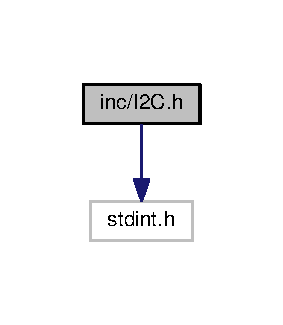
\includegraphics[width=136pt]{I2C_8h__incl}
\end{center}
\end{figure}
\subsection*{Functions}
\begin{DoxyCompactItemize}
\item 
void \hyperlink{I2C_8h_a84df9a5887b8b8230cfe85d18e53900e}{I2\+C\+\_\+\+Init} (void)
\begin{DoxyCompactList}\small\item\em initialize a I2C module with corresponding setting parameters. \end{DoxyCompactList}\item 
int \hyperlink{I2C_8h_aa2eca5eb27ebd77458e7584703467dde}{I2\+C\+\_\+read} (uint8\+\_\+t device\+Address, uint8\+\_\+t target\+Register, uint8\+\_\+t $\ast$data, uint32\+\_\+t count)
\begin{DoxyCompactList}\small\item\em read 1 or more bytes from slave device. \end{DoxyCompactList}\item 
int \hyperlink{I2C_8h_a45152120709fb4ad8a0d0f2f81f5f489}{I2\+C\+\_\+write} (uint8\+\_\+t device\+Address, uint8\+\_\+t target\+Register, uint8\+\_\+t $\ast$data, uint32\+\_\+t count)
\begin{DoxyCompactList}\small\item\em write 1 or more bytes to slave device. \end{DoxyCompactList}\item 
int \hyperlink{I2C_8h_a8596118ce5d9e43a3cde3bb9997bdb60}{I2\+C\+\_\+read\+\_\+byte} (uint8\+\_\+t device\+Address, uint8\+\_\+t target\+Register, uint8\+\_\+t $\ast$data)
\begin{DoxyCompactList}\small\item\em read 1 byte from slave device. \end{DoxyCompactList}\item 
int \hyperlink{I2C_8h_ad48380f04cae816c568f7ace0f39ccd6}{I2\+C\+\_\+write\+\_\+byte} (uint8\+\_\+t device\+Address, uint8\+\_\+t target\+Register, uint8\+\_\+t data)
\begin{DoxyCompactList}\small\item\em write 1 byte to slave device. \end{DoxyCompactList}\item 
int \hyperlink{I2C_8h_af86edfe5e765d79f017440af3e22209d}{I2\+C\+\_\+read\+\_\+2\+\_\+bytes} (uint8\+\_\+t device\+Address, uint8\+\_\+t target\+Register, uint8\+\_\+t $\ast$data)
\begin{DoxyCompactList}\small\item\em read 2 bytes from slave device. \end{DoxyCompactList}\item 
int \hyperlink{I2C_8h_ad5ea573eeb06a0314a5e36fdbe01303e}{I2\+C\+\_\+write\+\_\+2\+\_\+bytes} (uint8\+\_\+t device\+Address, uint8\+\_\+t target\+Register, uint8\+\_\+t $\ast$data)
\begin{DoxyCompactList}\small\item\em write 2 bytes to slave device. \end{DoxyCompactList}\item 
int \hyperlink{I2C_8h_ad5fbda826f261d78150bb95b9bcf5064}{I2\+C\+\_\+read\+\_\+4\+\_\+bytes} (uint8\+\_\+t device\+Address, uint8\+\_\+t target\+Register, uint8\+\_\+t $\ast$data)
\begin{DoxyCompactList}\small\item\em read 4 bytes from slave device. \end{DoxyCompactList}\item 
int \hyperlink{I2C_8h_a69bb29f4b4fd19ba304887847a945521}{I2\+C\+\_\+write\+\_\+4\+\_\+bytes} (uint8\+\_\+t device\+Address, uint8\+\_\+t target\+Register, uint8\+\_\+t $\ast$data)
\begin{DoxyCompactList}\small\item\em write 4 bytes to slave device. \end{DoxyCompactList}\end{DoxyCompactItemize}


\subsection{Detailed Description}
T\+M4\+C123G I2C A\+P\+Is and some settings. For future development and updates, please follow this repository\+: If you find any bug or problem, please create new issue or a pull request with a fix in the repository. Or you can simply email me about the problem or bug at \href{mailto:zeelivermorium@gmail.com}{\tt zeelivermorium@gmail.\+com} Much Appreciated! 

\begin{DoxyAuthor}{Author}
Zee Livermorium 
\end{DoxyAuthor}
\begin{DoxyDate}{Date}
Aug 4, 2018 
\end{DoxyDate}


\subsection{Function Documentation}
\index{I2\+C.\+h@{I2\+C.\+h}!I2\+C\+\_\+\+Init@{I2\+C\+\_\+\+Init}}
\index{I2\+C\+\_\+\+Init@{I2\+C\+\_\+\+Init}!I2\+C.\+h@{I2\+C.\+h}}
\subsubsection[{\texorpdfstring{I2\+C\+\_\+\+Init(void)}{I2C_Init(void)}}]{\setlength{\rightskip}{0pt plus 5cm}void I2\+C\+\_\+\+Init (
\begin{DoxyParamCaption}
\item[{void}]{}
\end{DoxyParamCaption}
)}\hypertarget{I2C_8h_a84df9a5887b8b8230cfe85d18e53900e}{}\label{I2C_8h_a84df9a5887b8b8230cfe85d18e53900e}


initialize a I2C module with corresponding setting parameters. 

I2\+C\+\_\+\+Init \index{I2\+C.\+h@{I2\+C.\+h}!I2\+C\+\_\+read@{I2\+C\+\_\+read}}
\index{I2\+C\+\_\+read@{I2\+C\+\_\+read}!I2\+C.\+h@{I2\+C.\+h}}
\subsubsection[{\texorpdfstring{I2\+C\+\_\+read(uint8\+\_\+t device\+Address, uint8\+\_\+t target\+Register, uint8\+\_\+t $\ast$data, uint32\+\_\+t count)}{I2C_read(uint8_t deviceAddress, uint8_t targetRegister, uint8_t *data, uint32_t count)}}]{\setlength{\rightskip}{0pt plus 5cm}int I2\+C\+\_\+read (
\begin{DoxyParamCaption}
\item[{uint8\+\_\+t}]{device\+Address, }
\item[{uint8\+\_\+t}]{target\+Register, }
\item[{uint8\+\_\+t $\ast$}]{data, }
\item[{uint32\+\_\+t}]{count}
\end{DoxyParamCaption}
)}\hypertarget{I2C_8h_aa2eca5eb27ebd77458e7584703467dde}{}\label{I2C_8h_aa2eca5eb27ebd77458e7584703467dde}


read 1 or more bytes from slave device. 

I2\+C\+\_\+read 
\begin{DoxyParams}{Parameters}
{\em device\+Address} & address of slave device. \\
\hline
{\em target\+Register} & target register of slave device. \\
\hline
{\em data} & data address to store read data. \\
\hline
{\em count} & number of bytes to be read. \\
\hline
\end{DoxyParams}
\index{I2\+C.\+h@{I2\+C.\+h}!I2\+C\+\_\+read\+\_\+2\+\_\+bytes@{I2\+C\+\_\+read\+\_\+2\+\_\+bytes}}
\index{I2\+C\+\_\+read\+\_\+2\+\_\+bytes@{I2\+C\+\_\+read\+\_\+2\+\_\+bytes}!I2\+C.\+h@{I2\+C.\+h}}
\subsubsection[{\texorpdfstring{I2\+C\+\_\+read\+\_\+2\+\_\+bytes(uint8\+\_\+t device\+Address, uint8\+\_\+t target\+Register, uint8\+\_\+t $\ast$data)}{I2C_read_2_bytes(uint8_t deviceAddress, uint8_t targetRegister, uint8_t *data)}}]{\setlength{\rightskip}{0pt plus 5cm}int I2\+C\+\_\+read\+\_\+2\+\_\+bytes (
\begin{DoxyParamCaption}
\item[{uint8\+\_\+t}]{device\+Address, }
\item[{uint8\+\_\+t}]{target\+Register, }
\item[{uint8\+\_\+t $\ast$}]{data}
\end{DoxyParamCaption}
)}\hypertarget{I2C_8h_af86edfe5e765d79f017440af3e22209d}{}\label{I2C_8h_af86edfe5e765d79f017440af3e22209d}


read 2 bytes from slave device. 

I2\+C\+\_\+read\+\_\+2\+\_\+bytes 
\begin{DoxyParams}{Parameters}
{\em device\+Address} & address of slave device. \\
\hline
{\em target\+Register} & target register of slave device. \\
\hline
{\em data} & data address to store read data. \\
\hline
\end{DoxyParams}
\index{I2\+C.\+h@{I2\+C.\+h}!I2\+C\+\_\+read\+\_\+4\+\_\+bytes@{I2\+C\+\_\+read\+\_\+4\+\_\+bytes}}
\index{I2\+C\+\_\+read\+\_\+4\+\_\+bytes@{I2\+C\+\_\+read\+\_\+4\+\_\+bytes}!I2\+C.\+h@{I2\+C.\+h}}
\subsubsection[{\texorpdfstring{I2\+C\+\_\+read\+\_\+4\+\_\+bytes(uint8\+\_\+t device\+Address, uint8\+\_\+t target\+Register, uint8\+\_\+t $\ast$data)}{I2C_read_4_bytes(uint8_t deviceAddress, uint8_t targetRegister, uint8_t *data)}}]{\setlength{\rightskip}{0pt plus 5cm}int I2\+C\+\_\+read\+\_\+4\+\_\+bytes (
\begin{DoxyParamCaption}
\item[{uint8\+\_\+t}]{device\+Address, }
\item[{uint8\+\_\+t}]{target\+Register, }
\item[{uint8\+\_\+t $\ast$}]{data}
\end{DoxyParamCaption}
)}\hypertarget{I2C_8h_ad5fbda826f261d78150bb95b9bcf5064}{}\label{I2C_8h_ad5fbda826f261d78150bb95b9bcf5064}


read 4 bytes from slave device. 

I2\+C\+\_\+read\+\_\+4\+\_\+bytes 
\begin{DoxyParams}{Parameters}
{\em device\+Address} & address of slave device. \\
\hline
{\em target\+Register} & target register of slave device. \\
\hline
{\em data} & data address to store read data. \\
\hline
\end{DoxyParams}
\index{I2\+C.\+h@{I2\+C.\+h}!I2\+C\+\_\+read\+\_\+byte@{I2\+C\+\_\+read\+\_\+byte}}
\index{I2\+C\+\_\+read\+\_\+byte@{I2\+C\+\_\+read\+\_\+byte}!I2\+C.\+h@{I2\+C.\+h}}
\subsubsection[{\texorpdfstring{I2\+C\+\_\+read\+\_\+byte(uint8\+\_\+t device\+Address, uint8\+\_\+t target\+Register, uint8\+\_\+t $\ast$data)}{I2C_read_byte(uint8_t deviceAddress, uint8_t targetRegister, uint8_t *data)}}]{\setlength{\rightskip}{0pt plus 5cm}int I2\+C\+\_\+read\+\_\+byte (
\begin{DoxyParamCaption}
\item[{uint8\+\_\+t}]{device\+Address, }
\item[{uint8\+\_\+t}]{target\+Register, }
\item[{uint8\+\_\+t $\ast$}]{data}
\end{DoxyParamCaption}
)}\hypertarget{I2C_8h_a8596118ce5d9e43a3cde3bb9997bdb60}{}\label{I2C_8h_a8596118ce5d9e43a3cde3bb9997bdb60}


read 1 byte from slave device. 

I2\+C\+\_\+read\+\_\+byte 
\begin{DoxyParams}{Parameters}
{\em device\+Address} & address of slave device. \\
\hline
{\em target\+Register} & target register of slave device. \\
\hline
{\em data} & data address to store read data. \\
\hline
\end{DoxyParams}
\index{I2\+C.\+h@{I2\+C.\+h}!I2\+C\+\_\+write@{I2\+C\+\_\+write}}
\index{I2\+C\+\_\+write@{I2\+C\+\_\+write}!I2\+C.\+h@{I2\+C.\+h}}
\subsubsection[{\texorpdfstring{I2\+C\+\_\+write(uint8\+\_\+t device\+Address, uint8\+\_\+t target\+Register, uint8\+\_\+t $\ast$data, uint32\+\_\+t count)}{I2C_write(uint8_t deviceAddress, uint8_t targetRegister, uint8_t *data, uint32_t count)}}]{\setlength{\rightskip}{0pt plus 5cm}int I2\+C\+\_\+write (
\begin{DoxyParamCaption}
\item[{uint8\+\_\+t}]{device\+Address, }
\item[{uint8\+\_\+t}]{target\+Register, }
\item[{uint8\+\_\+t $\ast$}]{data, }
\item[{uint32\+\_\+t}]{count}
\end{DoxyParamCaption}
)}\hypertarget{I2C_8h_a45152120709fb4ad8a0d0f2f81f5f489}{}\label{I2C_8h_a45152120709fb4ad8a0d0f2f81f5f489}


write 1 or more bytes to slave device. 

I2\+C\+\_\+write 
\begin{DoxyParams}{Parameters}
{\em device\+Address} & address of slave device. \\
\hline
{\em target\+Register} & target register of slave device. \\
\hline
{\em data} & data address of data to be writen. \\
\hline
{\em count} & number of bytes to be writen. \\
\hline
\end{DoxyParams}
\index{I2\+C.\+h@{I2\+C.\+h}!I2\+C\+\_\+write\+\_\+2\+\_\+bytes@{I2\+C\+\_\+write\+\_\+2\+\_\+bytes}}
\index{I2\+C\+\_\+write\+\_\+2\+\_\+bytes@{I2\+C\+\_\+write\+\_\+2\+\_\+bytes}!I2\+C.\+h@{I2\+C.\+h}}
\subsubsection[{\texorpdfstring{I2\+C\+\_\+write\+\_\+2\+\_\+bytes(uint8\+\_\+t device\+Address, uint8\+\_\+t target\+Register, uint8\+\_\+t $\ast$data)}{I2C_write_2_bytes(uint8_t deviceAddress, uint8_t targetRegister, uint8_t *data)}}]{\setlength{\rightskip}{0pt plus 5cm}int I2\+C\+\_\+write\+\_\+2\+\_\+bytes (
\begin{DoxyParamCaption}
\item[{uint8\+\_\+t}]{device\+Address, }
\item[{uint8\+\_\+t}]{target\+Register, }
\item[{uint8\+\_\+t $\ast$}]{data}
\end{DoxyParamCaption}
)}\hypertarget{I2C_8h_ad5ea573eeb06a0314a5e36fdbe01303e}{}\label{I2C_8h_ad5ea573eeb06a0314a5e36fdbe01303e}


write 2 bytes to slave device. 

I2\+C\+\_\+write\+\_\+2\+\_\+bytes 
\begin{DoxyParams}{Parameters}
{\em device\+Address} & address of slave device. \\
\hline
{\em target\+Register} & target register of slave device. \\
\hline
{\em data} & data to be writen. \\
\hline
\end{DoxyParams}
\index{I2\+C.\+h@{I2\+C.\+h}!I2\+C\+\_\+write\+\_\+4\+\_\+bytes@{I2\+C\+\_\+write\+\_\+4\+\_\+bytes}}
\index{I2\+C\+\_\+write\+\_\+4\+\_\+bytes@{I2\+C\+\_\+write\+\_\+4\+\_\+bytes}!I2\+C.\+h@{I2\+C.\+h}}
\subsubsection[{\texorpdfstring{I2\+C\+\_\+write\+\_\+4\+\_\+bytes(uint8\+\_\+t device\+Address, uint8\+\_\+t target\+Register, uint8\+\_\+t $\ast$data)}{I2C_write_4_bytes(uint8_t deviceAddress, uint8_t targetRegister, uint8_t *data)}}]{\setlength{\rightskip}{0pt plus 5cm}int I2\+C\+\_\+write\+\_\+4\+\_\+bytes (
\begin{DoxyParamCaption}
\item[{uint8\+\_\+t}]{device\+Address, }
\item[{uint8\+\_\+t}]{target\+Register, }
\item[{uint8\+\_\+t $\ast$}]{data}
\end{DoxyParamCaption}
)}\hypertarget{I2C_8h_a69bb29f4b4fd19ba304887847a945521}{}\label{I2C_8h_a69bb29f4b4fd19ba304887847a945521}


write 4 bytes to slave device. 

I2\+C\+\_\+write\+\_\+4\+\_\+bytes 
\begin{DoxyParams}{Parameters}
{\em device\+Address} & address of slave device. \\
\hline
{\em target\+Register} & target register of slave device. \\
\hline
{\em data} & data to be writen. \\
\hline
\end{DoxyParams}
\index{I2\+C.\+h@{I2\+C.\+h}!I2\+C\+\_\+write\+\_\+byte@{I2\+C\+\_\+write\+\_\+byte}}
\index{I2\+C\+\_\+write\+\_\+byte@{I2\+C\+\_\+write\+\_\+byte}!I2\+C.\+h@{I2\+C.\+h}}
\subsubsection[{\texorpdfstring{I2\+C\+\_\+write\+\_\+byte(uint8\+\_\+t device\+Address, uint8\+\_\+t target\+Register, uint8\+\_\+t data)}{I2C_write_byte(uint8_t deviceAddress, uint8_t targetRegister, uint8_t data)}}]{\setlength{\rightskip}{0pt plus 5cm}int I2\+C\+\_\+write\+\_\+byte (
\begin{DoxyParamCaption}
\item[{uint8\+\_\+t}]{device\+Address, }
\item[{uint8\+\_\+t}]{target\+Register, }
\item[{uint8\+\_\+t}]{data}
\end{DoxyParamCaption}
)}\hypertarget{I2C_8h_ad48380f04cae816c568f7ace0f39ccd6}{}\label{I2C_8h_ad48380f04cae816c568f7ace0f39ccd6}


write 1 byte to slave device. 

I2\+C\+\_\+write\+\_\+byte 
\begin{DoxyParams}{Parameters}
{\em device\+Address} & address of slave device. \\
\hline
{\em target\+Register} & target register of slave device. \\
\hline
{\em data} & data to be writen. \\
\hline
\end{DoxyParams}

\input{interpreter_8h}
\hypertarget{memprotect_8h}{}\section{inc/memprotect.h File Reference}
\label{memprotect_8h}\index{inc/memprotect.\+h@{inc/memprotect.\+h}}


Module implementing memory protection with the M\+PU.  


{\ttfamily \#include $<$stdint.\+h$>$}\\*
{\ttfamily \#include \char`\"{}tm4c123gh6pm.\+h\char`\"{}}\\*
Include dependency graph for memprotect.\+h\+:\nopagebreak
\begin{figure}[H]
\begin{center}
\leavevmode
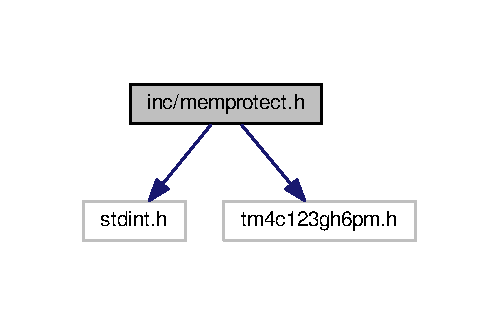
\includegraphics[width=240pt]{memprotect_8h__incl}
\end{center}
\end{figure}
\subsection*{Macros}
\begin{DoxyCompactItemize}
\item 
\#define \hyperlink{memprotect_8h_a95efeffea2dfd4dc18fd30325868332c}{A\+P\+\_\+\+P\+N\+A\+\_\+\+U\+NA}~(0)\hypertarget{memprotect_8h_a95efeffea2dfd4dc18fd30325868332c}{}\label{memprotect_8h_a95efeffea2dfd4dc18fd30325868332c}

\begin{DoxyCompactList}\small\item\em Privileged no access, unprivileged no access. \end{DoxyCompactList}\item 
\#define \hyperlink{memprotect_8h_a2a3f9f5e5b0eb24035bcadf75e66af68}{A\+P\+\_\+\+P\+R\+W\+\_\+\+U\+NA}~(1)\hypertarget{memprotect_8h_a2a3f9f5e5b0eb24035bcadf75e66af68}{}\label{memprotect_8h_a2a3f9f5e5b0eb24035bcadf75e66af68}

\begin{DoxyCompactList}\small\item\em Privileged r/w, unprivileged no access. \end{DoxyCompactList}\item 
\#define \hyperlink{memprotect_8h_a76e5d25531aff9d9f23508ddcb85a3be}{A\+P\+\_\+\+P\+R\+W\+\_\+\+U\+RO}~(2)\hypertarget{memprotect_8h_a76e5d25531aff9d9f23508ddcb85a3be}{}\label{memprotect_8h_a76e5d25531aff9d9f23508ddcb85a3be}

\begin{DoxyCompactList}\small\item\em Privileged r/w, unprivileged read-\/only. \end{DoxyCompactList}\item 
\#define \hyperlink{memprotect_8h_a3cd351e57cea87e082fc92d1b8658152}{A\+P\+\_\+\+P\+R\+W\+\_\+\+U\+RW}~(3)\hypertarget{memprotect_8h_a3cd351e57cea87e082fc92d1b8658152}{}\label{memprotect_8h_a3cd351e57cea87e082fc92d1b8658152}

\begin{DoxyCompactList}\small\item\em Privileged r/w, unprivileged r/w. \end{DoxyCompactList}\item 
\#define \hyperlink{memprotect_8h_a0737c5405b4bc3077aa2a0399f6b4fb8}{A\+P\+\_\+\+P\+R\+O\+\_\+\+U\+NA}~(5)\hypertarget{memprotect_8h_a0737c5405b4bc3077aa2a0399f6b4fb8}{}\label{memprotect_8h_a0737c5405b4bc3077aa2a0399f6b4fb8}

\begin{DoxyCompactList}\small\item\em Privileged read-\/only, unprivileged no access. \end{DoxyCompactList}\item 
\#define \hyperlink{memprotect_8h_ab318812251e2dc42bd1eeb226c672e4e}{A\+P\+\_\+\+P\+R\+O\+\_\+\+U\+RO}~(6)\hypertarget{memprotect_8h_ab318812251e2dc42bd1eeb226c672e4e}{}\label{memprotect_8h_ab318812251e2dc42bd1eeb226c672e4e}

\begin{DoxyCompactList}\small\item\em Privileged read-\/only, unprivileged read-\/only. \end{DoxyCompactList}\end{DoxyCompactItemize}


\subsection{Detailed Description}
Module implementing memory protection with the M\+PU. 

\begin{DoxyAuthor}{Author}
Riley Wood (\href{mailto:riley.wood@utexas.edu}{\tt riley.\+wood@utexas.\+edu}) 
\end{DoxyAuthor}
\begin{DoxyVersion}{Version}
0.\+1
\end{DoxyVersion}
\begin{DoxyCopyright}{Copyright}
Copyright (c) 2019 
\end{DoxyCopyright}

\input{misc__macros_8h}
\hypertarget{motors_8h}{}\section{inc/motors.h File Reference}
\label{motors_8h}\index{inc/motors.\+h@{inc/motors.\+h}}


Interface to two DC motors controlled by P\+WM. Allows differential driving.  


{\ttfamily \#include $<$stdint.\+h$>$}\\*
Include dependency graph for motors.\+h\+:\nopagebreak
\begin{figure}[H]
\begin{center}
\leavevmode
\includegraphics[width=151pt]{motors_8h__incl}
\end{center}
\end{figure}
\subsection*{Functions}
\begin{DoxyCompactItemize}
\item 
void \hyperlink{motors_8h_a5c0d48e46db133698dad2cbf5df21486}{Motors\+\_\+\+Init} (void)\hypertarget{motors_8h_a5c0d48e46db133698dad2cbf5df21486}{}\label{motors_8h_a5c0d48e46db133698dad2cbf5df21486}

\begin{DoxyCompactList}\small\item\em Initialize the robot motors. \end{DoxyCompactList}\item 
void \hyperlink{motors_8h_a1156160dc9b3c27db38c8c4b90c12caa}{Motors\+\_\+\+Set\+Torque} (int16\+\_\+t left\+\_\+trq, int16\+\_\+t right\+\_\+trq)
\begin{DoxyCompactList}\small\item\em Set the torque for each of the two motors atomically. \end{DoxyCompactList}\item 
void \hyperlink{motors_8h_aa71622b5e7e99d500b3f51066cea701c}{Motors\+\_\+\+Set\+Torque\+\_\+\+Left} (int16\+\_\+t left\+\_\+trq)
\begin{DoxyCompactList}\small\item\em Set the torque of the left motor individually. \end{DoxyCompactList}\item 
void \hyperlink{motors_8h_a5749c819b9d4d966fc5a6f7730b18850}{Motors\+\_\+\+Set\+Torque\+\_\+\+Right} (int16\+\_\+t right\+\_\+trq)
\begin{DoxyCompactList}\small\item\em Set the torque of the left motor individually. \end{DoxyCompactList}\item 
void \hyperlink{motors_8h_ac35a70f74e7097175bee3ad296713d33}{Motors\+\_\+\+Brake} (void)\hypertarget{motors_8h_ac35a70f74e7097175bee3ad296713d33}{}\label{motors_8h_ac35a70f74e7097175bee3ad296713d33}

\begin{DoxyCompactList}\small\item\em Brake both motors (tie both motors\textquotesingle{} leads to ground) \end{DoxyCompactList}\item 
void \hyperlink{motors_8h_a0ddfe47225418fa87ef927b7935ccb0a}{Motors\+\_\+\+Brake\+\_\+\+Left} (void)\hypertarget{motors_8h_a0ddfe47225418fa87ef927b7935ccb0a}{}\label{motors_8h_a0ddfe47225418fa87ef927b7935ccb0a}

\begin{DoxyCompactList}\small\item\em Brake left motor (tie motor leads to ground) \end{DoxyCompactList}\item 
void \hyperlink{motors_8h_a04d533dd786973adc8c59ea77a96c111}{Motors\+\_\+\+Brake\+\_\+\+Right} (void)\hypertarget{motors_8h_a04d533dd786973adc8c59ea77a96c111}{}\label{motors_8h_a04d533dd786973adc8c59ea77a96c111}

\begin{DoxyCompactList}\small\item\em Brake right motor (tie motor leads to ground) \end{DoxyCompactList}\end{DoxyCompactItemize}


\subsection{Detailed Description}
Interface to two DC motors controlled by P\+WM. Allows differential driving. 

\begin{DoxyAuthor}{Author}
Riley Wood (\href{mailto:riley.wood@utexas.edu}{\tt riley.\+wood@utexas.\+edu})
\end{DoxyAuthor}
This library makes use of P\+WM module 0, outputs 0 and 3. These are produced by P\+WM module 0\textquotesingle{}s generators numbered 0 and 1.

Conventions\+:
\begin{DoxyItemize}
\item Definition of \char`\"{}left\char`\"{} versus \char`\"{}right\char`\"{}\+:
\begin{DoxyItemize}
\item The \char`\"{}left motor\char`\"{} is the motor on your left when the robot is on the ground with the servo pointed away from you.
\item The \char`\"{}right motor\char`\"{} is the motor on your right when the robot is on the ground with the servo pointed away from you.
\end{DoxyItemize}
\item How to connect motors to motor board\+:
\begin{DoxyItemize}
\item The left motor must be connected to motor port A.
\item The right motor must be connected to motor port B.
\end{DoxyItemize}
\item Motor pin assignments\+:
\begin{DoxyItemize}
\item The red wire of the left motor will be connected to A-\/ and is controlled by P\+B6
\item The black wire of the left motor will be connected to A+ and is controlled by P\+B7
\item The red wire of right motor will be connected to B-\/ and is controlled by P\+B4
\item The black wire of the right motor will be connected to B+ and is controlled by P\+B5
\end{DoxyItemize}
\item Pin configurations\+:
\begin{DoxyItemize}
\item A-\/ (P\+B6) and B+ (P\+B5) will be configured as P\+WM outputs
\item A+ (P\+B7) and B-\/ (P\+B4) will be configured as digital outputs.
\item We alternate + and -\/ so that when both motors are driving forward (i.\+e. they are rotating O\+P\+P\+O\+S\+I\+TE directions) with the same torque, their digital and P\+WM output configurations will be identical.
\end{DoxyItemize}
\item H-\/\+Bridge convention\+:
\begin{DoxyItemize}
\item A value of 1 (high) on any of P\+B4/5/6/7 will connect the corresponding motor terminal (A/\+B/+/-\/) to battery power.
\item A value of 0 (low) on any of P\+B4/5/6/7 will connect the corresponding motor terminal (A/\+B/+/-\/) to ground.
\end{DoxyItemize}
\end{DoxyItemize}

\begin{DoxyCopyright}{Copyright}
Copyright (c) 2019 
\end{DoxyCopyright}


\subsection{Function Documentation}
\index{motors.\+h@{motors.\+h}!Motors\+\_\+\+Set\+Torque@{Motors\+\_\+\+Set\+Torque}}
\index{Motors\+\_\+\+Set\+Torque@{Motors\+\_\+\+Set\+Torque}!motors.\+h@{motors.\+h}}
\subsubsection[{\texorpdfstring{Motors\+\_\+\+Set\+Torque(int16\+\_\+t left\+\_\+trq, int16\+\_\+t right\+\_\+trq)}{Motors_SetTorque(int16_t left_trq, int16_t right_trq)}}]{\setlength{\rightskip}{0pt plus 5cm}void Motors\+\_\+\+Set\+Torque (
\begin{DoxyParamCaption}
\item[{int16\+\_\+t}]{left\+\_\+trq, }
\item[{int16\+\_\+t}]{right\+\_\+trq}
\end{DoxyParamCaption}
)}\hypertarget{motors_8h_a1156160dc9b3c27db38c8c4b90c12caa}{}\label{motors_8h_a1156160dc9b3c27db38c8c4b90c12caa}


Set the torque for each of the two motors atomically. 


\begin{DoxyParams}{Parameters}
{\em left\+\_\+trq} & Torque for left motor. Between -\/1000 and 1000. Positive argument indicates forward motion of robot, negative indicates backward. Zero indicates no rotation. \\
\hline
{\em right\+\_\+trq} & Torque for right motor. Between -\/1000 and 1000. Positive argument indicates forward motion of robot, negative indicates backward. Zero indicates no rotation. \\
\hline
\end{DoxyParams}
\index{motors.\+h@{motors.\+h}!Motors\+\_\+\+Set\+Torque\+\_\+\+Left@{Motors\+\_\+\+Set\+Torque\+\_\+\+Left}}
\index{Motors\+\_\+\+Set\+Torque\+\_\+\+Left@{Motors\+\_\+\+Set\+Torque\+\_\+\+Left}!motors.\+h@{motors.\+h}}
\subsubsection[{\texorpdfstring{Motors\+\_\+\+Set\+Torque\+\_\+\+Left(int16\+\_\+t left\+\_\+trq)}{Motors_SetTorque_Left(int16_t left_trq)}}]{\setlength{\rightskip}{0pt plus 5cm}void Motors\+\_\+\+Set\+Torque\+\_\+\+Left (
\begin{DoxyParamCaption}
\item[{int16\+\_\+t}]{left\+\_\+trq}
\end{DoxyParamCaption}
)}\hypertarget{motors_8h_aa71622b5e7e99d500b3f51066cea701c}{}\label{motors_8h_aa71622b5e7e99d500b3f51066cea701c}


Set the torque of the left motor individually. 


\begin{DoxyParams}{Parameters}
{\em left\+\_\+trq} & Torque for left motor. Between -\/1000 and 1000. Positive argument indicates forward motion of robot, negative indicates backward. Zero indicates no rotation. \\
\hline
\end{DoxyParams}
\index{motors.\+h@{motors.\+h}!Motors\+\_\+\+Set\+Torque\+\_\+\+Right@{Motors\+\_\+\+Set\+Torque\+\_\+\+Right}}
\index{Motors\+\_\+\+Set\+Torque\+\_\+\+Right@{Motors\+\_\+\+Set\+Torque\+\_\+\+Right}!motors.\+h@{motors.\+h}}
\subsubsection[{\texorpdfstring{Motors\+\_\+\+Set\+Torque\+\_\+\+Right(int16\+\_\+t right\+\_\+trq)}{Motors_SetTorque_Right(int16_t right_trq)}}]{\setlength{\rightskip}{0pt plus 5cm}void Motors\+\_\+\+Set\+Torque\+\_\+\+Right (
\begin{DoxyParamCaption}
\item[{int16\+\_\+t}]{right\+\_\+trq}
\end{DoxyParamCaption}
)}\hypertarget{motors_8h_a5749c819b9d4d966fc5a6f7730b18850}{}\label{motors_8h_a5749c819b9d4d966fc5a6f7730b18850}


Set the torque of the left motor individually. 


\begin{DoxyParams}{Parameters}
{\em right\+\_\+trq} & Torque for right motor. Between -\/1000 and 1000. Positive argument indicates forward motion of robot, negative indicates backward. Zero indicates no rotation. \\
\hline
\end{DoxyParams}

\hypertarget{OS_8h}{}\section{inc/\+OS.h File Reference}
\label{OS_8h}\index{inc/\+O\+S.\+h@{inc/\+O\+S.\+h}}


Real Time Operating System for Labs 2 and 3 E\+E445\+M/\+E\+E380\+L.\+12.  


{\ttfamily \#include $<$stdint.\+h$>$}\\*
{\ttfamily \#include \char`\"{}heap.\+h\char`\"{}}\\*
Include dependency graph for O\+S.\+h\+:\nopagebreak
\begin{figure}[H]
\begin{center}
\leavevmode
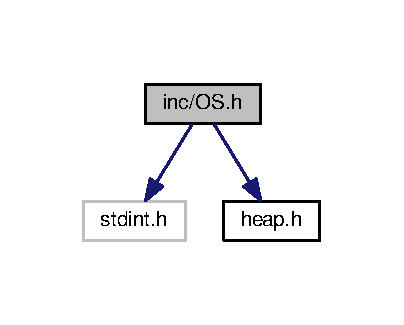
\includegraphics[width=194pt]{OS_8h__incl}
\end{center}
\end{figure}
This graph shows which files directly or indirectly include this file\+:\nopagebreak
\begin{figure}[H]
\begin{center}
\leavevmode
\includegraphics[width=176pt]{OS_8h__dep__incl}
\end{center}
\end{figure}
\subsection*{Data Structures}
\begin{DoxyCompactItemize}
\item 
struct \hyperlink{struct__pcb__s}{\+\_\+pcb\+\_\+s}
\item 
struct \hyperlink{struct__tcb__s}{\+\_\+tcb\+\_\+s}
\item 
struct \hyperlink{structSema4}{Sema4}
\end{DoxyCompactItemize}
\subsection*{Macros}
\begin{DoxyCompactItemize}
\item 
\#define {\bfseries T\+I\+M\+E\+\_\+1\+MS}~80000\hypertarget{OS_8h_ad6445469b3084b0c8a8ea272e8a40a17}{}\label{OS_8h_ad6445469b3084b0c8a8ea272e8a40a17}

\item 
\#define {\bfseries T\+I\+M\+E\+\_\+2\+MS}~(2 $\ast$ T\+I\+M\+E\+\_\+1\+MS)\hypertarget{OS_8h_a601fb0d91385070bae69c2b1c4e63162}{}\label{OS_8h_a601fb0d91385070bae69c2b1c4e63162}

\item 
\#define {\bfseries T\+I\+M\+E\+\_\+500\+US}~(T\+I\+M\+E\+\_\+1\+MS / 2)\hypertarget{OS_8h_a5bd8a6024a3e7cd43b7fe30988ca81e8}{}\label{OS_8h_a5bd8a6024a3e7cd43b7fe30988ca81e8}

\item 
\#define {\bfseries T\+I\+M\+E\+\_\+250\+US}~(T\+I\+M\+E\+\_\+1\+MS / 4)\hypertarget{OS_8h_aae4936d8a1bad649da44cacada40b157}{}\label{OS_8h_aae4936d8a1bad649da44cacada40b157}

\item 
\#define {\bfseries T\+C\+B\+\_\+\+M\+A\+G\+IC}~(0x900d900d)\hypertarget{OS_8h_a0fb8aa2f0ea0a6494f1639dd97087013}{}\label{OS_8h_a0fb8aa2f0ea0a6494f1639dd97087013}

\item 
\#define \hyperlink{OS_8h_accb79b9446dd2b953a1fb8437c5f6e15}{O\+S\+\_\+\+Add\+Thread}(task,  stack\+Size,  priority)
\item 
\#define \hyperlink{OS_8h_adf56561acbee98b34e8c42ff6b147255}{O\+S\+\_\+\+Add\+Periodic\+Thread}(task,  period,  priority)~O\+S\+\_\+\+Add\+Periodic\+Thread\+\_\+priv(task, period, priority, \#task)
\end{DoxyCompactItemize}
\subsection*{Typedefs}
\begin{DoxyCompactItemize}
\item 
typedef struct \hyperlink{struct__pcb__s}{\+\_\+pcb\+\_\+s} {\bfseries pcb\+\_\+t}\hypertarget{OS_8h_add17966847109f7551977a87ddfcd8aa}{}\label{OS_8h_add17966847109f7551977a87ddfcd8aa}

\item 
typedef struct \hyperlink{struct__tcb__s}{\+\_\+tcb\+\_\+s} {\bfseries tcb\+\_\+t}\hypertarget{OS_8h_a5f5b511a2a589828581399459da62c6a}{}\label{OS_8h_a5f5b511a2a589828581399459da62c6a}

\item 
typedef struct \hyperlink{structSema4}{Sema4} {\bfseries Sema4\+Type}\hypertarget{OS_8h_a798fbe37dbc49a5ff9af51bf7de1ee8e}{}\label{OS_8h_a798fbe37dbc49a5ff9af51bf7de1ee8e}

\end{DoxyCompactItemize}
\subsection*{Functions}
\begin{DoxyCompactItemize}
\item 
void \hyperlink{OS_8h_acb6df8f47f418aad9c9a9e045d7d1e6d}{O\+S\+\_\+\+Init} (void)
\item 
void \hyperlink{OS_8h_af580c6222330cc3d214763ddac7800b9}{O\+S\+\_\+\+Init\+Semaphore} (\hyperlink{structSema4}{Sema4\+Type} $\ast$sema\+Pt, long value)
\item 
void \hyperlink{OS_8h_aad29612829941c857ed685f40e193cd0}{O\+S\+\_\+\+Wait} (\hyperlink{structSema4}{Sema4\+Type} $\ast$sema\+Pt)
\item 
void \hyperlink{OS_8h_a0c4d587c411a23652529110910261fde}{O\+S\+\_\+\+Signal} (\hyperlink{structSema4}{Sema4\+Type} $\ast$sema\+Pt)
\item 
void \hyperlink{OS_8h_a3f127f7a40ffd3e43b7b0f4c8b7f30ff}{O\+S\+\_\+b\+Wait} (\hyperlink{structSema4}{Sema4\+Type} $\ast$sema\+Pt)
\item 
void \hyperlink{OS_8h_aacf0c377b570fc63b103c57e0fbc7acd}{O\+S\+\_\+b\+Signal} (\hyperlink{structSema4}{Sema4\+Type} $\ast$sema\+Pt)
\item 
void \hyperlink{OS_8h_a075cf7301361417f66be1d5c22e36b0f}{Jitter} (void)\hypertarget{OS_8h_a075cf7301361417f66be1d5c22e36b0f}{}\label{OS_8h_a075cf7301361417f66be1d5c22e36b0f}

\begin{DoxyCompactList}\small\item\em Print the max periodic task jitter measured thus far to the S\+T7735 display. \end{DoxyCompactList}\item 
int {\bfseries \+\_\+\+\_\+\+O\+S\+\_\+\+Add\+Thread} (void($\ast$task)(void), unsigned long stack\+Size, unsigned long priority, char $\ast$task\+\_\+name, \hyperlink{struct__pcb__s}{pcb\+\_\+t} $\ast$parent\+\_\+process)\hypertarget{OS_8h_a3e5c42edf8d08a40ccdee09e200d84b6}{}\label{OS_8h_a3e5c42edf8d08a40ccdee09e200d84b6}

\item 
int {\bfseries O\+S\+\_\+\+S\+V\+C\+\_\+\+Add\+Thread} (void($\ast$task)(void), unsigned long stack\+Size, unsigned long priority)\hypertarget{OS_8h_a5ada4dffc21eb52b004d3bdbfa4fa001}{}\label{OS_8h_a5ada4dffc21eb52b004d3bdbfa4fa001}

\item 
unsigned long \hyperlink{OS_8h_adc21b8aab03cbb1611186ca3ac9123d8}{O\+S\+\_\+\+Id} (void)
\item 
unsigned long {\bfseries O\+S\+\_\+\+S\+V\+C\+\_\+\+Id} (void)\hypertarget{OS_8h_a45ee1a7efb9a8715e6e012d661ee23e9}{}\label{OS_8h_a45ee1a7efb9a8715e6e012d661ee23e9}

\item 
int {\bfseries O\+S\+\_\+\+Add\+Periodic\+Thread\+\_\+priv} (void($\ast$task)(void), unsigned long period, unsigned long priority, char $\ast$task\+\_\+name)\hypertarget{OS_8h_a21ee017683a4a2b593d5497a27addac0}{}\label{OS_8h_a21ee017683a4a2b593d5497a27addac0}

\item 
int \hyperlink{OS_8h_a5c387e683842fc4f9f846729a60186da}{O\+S\+\_\+\+Add\+S\+W1\+Task} (void($\ast$task)(void), unsigned long priority)
\item 
int \hyperlink{OS_8h_a508ed7f6202df8a9e500994ad4399784}{O\+S\+\_\+\+Add\+S\+W2\+Task} (void($\ast$task)(void), unsigned long priority)
\item 
void \hyperlink{OS_8h_aeeb2aca9e1a16738a5d82353b2d497ac}{O\+S\+\_\+\+Sleep} (unsigned long sleep\+Time)
\item 
void {\bfseries O\+S\+\_\+\+S\+V\+C\+\_\+\+Sleep} (unsigned long sleep\+Time)\hypertarget{OS_8h_a63c0c2c5a2ee62b852b102d84138e090}{}\label{OS_8h_a63c0c2c5a2ee62b852b102d84138e090}

\item 
void \hyperlink{OS_8h_a8e991f4f2576c5cfec04ef5f37aabea5}{O\+S\+\_\+\+Kill} (void)
\item 
void {\bfseries O\+S\+\_\+\+S\+V\+C\+\_\+\+Kill} (void)\hypertarget{OS_8h_a88f4da88fb76c8d916fb1f7150c57231}{}\label{OS_8h_a88f4da88fb76c8d916fb1f7150c57231}

\item 
void \hyperlink{OS_8h_a4e71587568a2a48931a35615cad1b5db}{O\+S\+\_\+\+Suspend} (void)
\item 
void {\bfseries O\+S\+\_\+\+S\+V\+C\+\_\+\+Suspend} (void)\hypertarget{OS_8h_a10bb4fa6889dd532a4ec5f61a1cd0726}{}\label{OS_8h_a10bb4fa6889dd532a4ec5f61a1cd0726}

\item 
void \hyperlink{OS_8h_a361ff1137f5dad8e0a74631be6fb12b6}{O\+S\+\_\+\+Fifo\+\_\+\+Init} (unsigned long size)
\item 
int \hyperlink{OS_8h_adf231073602c9328f6248f6272d63e7f}{O\+S\+\_\+\+Fifo\+\_\+\+Put} (unsigned long data)
\item 
unsigned long \hyperlink{OS_8h_af899a42296039e22ffdd8bf6e1ca208e}{O\+S\+\_\+\+Fifo\+\_\+\+Get} (void)
\item 
long \hyperlink{OS_8h_a9ff4cb899801f20ff90cbf2717c154c7}{O\+S\+\_\+\+Fifo\+\_\+\+Size} (void)
\item 
void \hyperlink{OS_8h_a84e1a933dd73e319fdd5649c2270281b}{O\+S\+\_\+\+Mail\+Box\+\_\+\+Init} (void)
\item 
void \hyperlink{OS_8h_ac4c3ebdb61c0c11195d6fcafeb0d4c99}{O\+S\+\_\+\+Mail\+Box\+\_\+\+Send} (unsigned long data)
\item 
unsigned long \hyperlink{OS_8h_ace71083584f0f1e5e2f081f1e4a1394a}{O\+S\+\_\+\+Mail\+Box\+\_\+\+Recv} (void)
\item 
unsigned long long \hyperlink{OS_8h_a5798d7fa05a4c3a523efe1b5651c5318}{O\+S\+\_\+\+Time} (void)
\item 
unsigned long long {\bfseries O\+S\+\_\+\+S\+V\+C\+\_\+\+Time} (void)\hypertarget{OS_8h_a379b84d99f5b3ba7d872153fafbe3335}{}\label{OS_8h_a379b84d99f5b3ba7d872153fafbe3335}

\item 
unsigned long long \hyperlink{OS_8h_af4b27f93116607bd3986125cb1c9edcf}{O\+S\+\_\+\+Time\+Difference} (unsigned long long start, unsigned long long stop)
\item 
void \hyperlink{OS_8h_ace6ec4b7947542f7d7ff3104d8c759bd}{O\+S\+\_\+\+Clear\+Ms\+Time} (void)
\item 
unsigned long \hyperlink{OS_8h_a251073790d2782617fd7474625761573}{O\+S\+\_\+\+Ms\+Time} (void)
\item 
void \hyperlink{OS_8h_a18553a7e1d82dcaaeb80a5524bd01cf2}{O\+S\+\_\+\+Launch} (unsigned long the\+Time\+Slice)
\item 
int \hyperlink{OS_8h_a3271236396a143a19c9650377e0f32ee}{O\+S\+\_\+\+Add\+Process} (void($\ast$entry)(void), void $\ast$text, void $\ast$data, unsigned long stack\+Size, unsigned long priority)
\begin{DoxyCompactList}\small\item\em Launch a process in the OS. \end{DoxyCompactList}\item 
long {\bfseries Start\+Critical} (void)\hypertarget{OS_8h_a6e7e2088607214bc15b17ac57b57df1b}{}\label{OS_8h_a6e7e2088607214bc15b17ac57b57df1b}

\item 
void {\bfseries End\+Critical} (long sr)\hypertarget{OS_8h_a670da3ff1aea0c7d54c40e9e40b5eeed}{}\label{OS_8h_a670da3ff1aea0c7d54c40e9e40b5eeed}

\item 
void {\bfseries Disable\+Interrupts} (void)\hypertarget{OS_8h_ac866dbaf7b167e5c46bb33de42eee84d}{}\label{OS_8h_ac866dbaf7b167e5c46bb33de42eee84d}

\item 
void {\bfseries Enable\+Interrupts} (void)\hypertarget{OS_8h_ab712356331a62b04aebcb373865e68c4}{}\label{OS_8h_ab712356331a62b04aebcb373865e68c4}

\end{DoxyCompactItemize}
\subsection*{Variables}
\begin{DoxyCompactItemize}
\item 
\hyperlink{struct__tcb__s}{tcb\+\_\+t} $\ast$ {\bfseries cur\+\_\+tcb}\hypertarget{OS_8h_aa1c72d659051f84119a2c6373fe43bee}{}\label{OS_8h_aa1c72d659051f84119a2c6373fe43bee}

\end{DoxyCompactItemize}


\subsection{Detailed Description}
Real Time Operating System for Labs 2 and 3 E\+E445\+M/\+E\+E380\+L.\+12. 

R\+T\+OS kernel capable of round-\/robin scheduling, up to 2 low-\/jitter periodic tasks.

Reserves W\+T\+I\+M\+E\+R1A and B for periodic task scheduling. Reserves Sys\+Tick timer for round-\/robin scheduling. Reserves W\+T\+I\+M\+E\+R0 as a 64-\/bit time source.

Interface by Jonathan W. Valvano 2/20/17, \href{mailto:valvano@mail.utexas.edu}{\tt valvano@mail.\+utexas.\+edu} Implementation by Riley Wood and Jeageun Jung \begin{DoxyAuthor}{Author}
Riley Wood and Jeageun Jung 
\end{DoxyAuthor}


\subsection{Macro Definition Documentation}
\index{O\+S.\+h@{O\+S.\+h}!O\+S\+\_\+\+Add\+Periodic\+Thread@{O\+S\+\_\+\+Add\+Periodic\+Thread}}
\index{O\+S\+\_\+\+Add\+Periodic\+Thread@{O\+S\+\_\+\+Add\+Periodic\+Thread}!O\+S.\+h@{O\+S.\+h}}
\subsubsection[{\texorpdfstring{O\+S\+\_\+\+Add\+Periodic\+Thread}{OS_AddPeriodicThread}}]{\setlength{\rightskip}{0pt plus 5cm}\#define O\+S\+\_\+\+Add\+Periodic\+Thread(
\begin{DoxyParamCaption}
\item[{}]{task, }
\item[{}]{period, }
\item[{}]{priority}
\end{DoxyParamCaption}
)~O\+S\+\_\+\+Add\+Periodic\+Thread\+\_\+priv(task, period, priority, \#task)}\hypertarget{OS_8h_adf56561acbee98b34e8c42ff6b147255}{}\label{OS_8h_adf56561acbee98b34e8c42ff6b147255}
Add a background periodic task. Typically this function receives the highest priority You are free to select the time resolution for this function It is assumed that the user task will run to completion and return This task can not spin, block, loop, sleep, or kill This task can call O\+S\+\_\+\+Signal O\+S\+\_\+b\+Signal O\+S\+\_\+\+Add\+Thread This task does not have a Thread ID In lab 2, this command will be called 0 or 1 times In lab 2, the priority field can be ignored In lab 3, this command will be called 0 1 or 2 times In lab 3, there will be up to four background threads, and this priority field determines the relative priority of these four threads 
\begin{DoxyParams}{Parameters}
{\em task} & pointer to a void/void background function \\
\hline
{\em period} & given in system time units (12.\+5ns) \\
\hline
{\em priority} & 0 is the highest, 5 is the lowest \\
\hline
\end{DoxyParams}
\begin{DoxyReturn}{Returns}
1 if successful, 0 if this thread can not be added 
\end{DoxyReturn}
\index{O\+S.\+h@{O\+S.\+h}!O\+S\+\_\+\+Add\+Thread@{O\+S\+\_\+\+Add\+Thread}}
\index{O\+S\+\_\+\+Add\+Thread@{O\+S\+\_\+\+Add\+Thread}!O\+S.\+h@{O\+S.\+h}}
\subsubsection[{\texorpdfstring{O\+S\+\_\+\+Add\+Thread}{OS_AddThread}}]{\setlength{\rightskip}{0pt plus 5cm}\#define O\+S\+\_\+\+Add\+Thread(
\begin{DoxyParamCaption}
\item[{}]{task, }
\item[{}]{stack\+Size, }
\item[{}]{priority}
\end{DoxyParamCaption}
)}\hypertarget{OS_8h_accb79b9446dd2b953a1fb8437c5f6e15}{}\label{OS_8h_accb79b9446dd2b953a1fb8437c5f6e15}
{\bfseries Value\+:}
\begin{DoxyCode}
\_\_OS\_AddThread(task,\(\backslash\)
                                                               stackSize,\(\backslash\)
                                                               priority,\(\backslash\)
                                                               #task,\(\backslash\)
                                                               cur\_tcb ? cur\_tcb->parent\_process : 0)
\end{DoxyCode}
add a foregound thread to the scheduler stack size must be divisable by 8 (aligned to double word boundary) In Lab 2, you can ignore both the stack\+Size and priority fields In Lab 3, you can ignore the stack\+Size fields 
\begin{DoxyParams}{Parameters}
{\em task} & Task function \\
\hline
{\em stack\+Size} & Size of the stack in bytes. Should be divisible by 8 \\
\hline
{\em priority} & Priority of the task. 0 is highest, 5 is lowest. \\
\hline
\end{DoxyParams}
\begin{DoxyReturn}{Returns}
1 if successful, 0 if this thread can not be added 
\end{DoxyReturn}


\subsection{Function Documentation}
\index{O\+S.\+h@{O\+S.\+h}!O\+S\+\_\+\+Add\+Process@{O\+S\+\_\+\+Add\+Process}}
\index{O\+S\+\_\+\+Add\+Process@{O\+S\+\_\+\+Add\+Process}!O\+S.\+h@{O\+S.\+h}}
\subsubsection[{\texorpdfstring{O\+S\+\_\+\+Add\+Process(void($\ast$entry)(void), void $\ast$text, void $\ast$data, unsigned long stack\+Size, unsigned long priority)}{OS_AddProcess(void(*entry)(void), void *text, void *data, unsigned long stackSize, unsigned long priority)}}]{\setlength{\rightskip}{0pt plus 5cm}int O\+S\+\_\+\+Add\+Process (
\begin{DoxyParamCaption}
\item[{void($\ast$)(void)}]{entry, }
\item[{void $\ast$}]{text, }
\item[{void $\ast$}]{data, }
\item[{unsigned long}]{stack\+Size, }
\item[{unsigned long}]{priority}
\end{DoxyParamCaption}
)}\hypertarget{OS_8h_a3271236396a143a19c9650377e0f32ee}{}\label{OS_8h_a3271236396a143a19c9650377e0f32ee}


Launch a process in the OS. 


\begin{DoxyParams}{Parameters}
{\em entry} & Entry point, usually main() of the process \\
\hline
{\em text} & Text (code) section start address \\
\hline
{\em data} & Data section start address \\
\hline
{\em stack\+Size} & Size of the stack for the first thread \\
\hline
{\em priority} & Priority for the first thread \\
\hline
\end{DoxyParams}
\begin{DoxyReturn}{Returns}
int 0 on success, -\/1 on failure. 
\end{DoxyReturn}
\index{O\+S.\+h@{O\+S.\+h}!O\+S\+\_\+\+Add\+S\+W1\+Task@{O\+S\+\_\+\+Add\+S\+W1\+Task}}
\index{O\+S\+\_\+\+Add\+S\+W1\+Task@{O\+S\+\_\+\+Add\+S\+W1\+Task}!O\+S.\+h@{O\+S.\+h}}
\subsubsection[{\texorpdfstring{O\+S\+\_\+\+Add\+S\+W1\+Task(void($\ast$task)(void), unsigned long priority)}{OS_AddSW1Task(void(*task)(void), unsigned long priority)}}]{\setlength{\rightskip}{0pt plus 5cm}int O\+S\+\_\+\+Add\+S\+W1\+Task (
\begin{DoxyParamCaption}
\item[{void($\ast$)(void)}]{task, }
\item[{unsigned long}]{priority}
\end{DoxyParamCaption}
)}\hypertarget{OS_8h_a5c387e683842fc4f9f846729a60186da}{}\label{OS_8h_a5c387e683842fc4f9f846729a60186da}
add a background task to run whenever the S\+W1 (P\+F4) button is pushed 
\begin{DoxyParams}{Parameters}
{\em pointer} & to a void/void background function \\
\hline
{\em priority} & 0 is the highest, 5 is the lowest \\
\hline
\end{DoxyParams}
\begin{DoxyReturn}{Returns}
1 if successful, 0 if this thread can not be added It is assumed that the user task will run to completion and return This task can not spin, block, loop, sleep, or kill This task can call O\+S\+\_\+\+Signal O\+S\+\_\+b\+Signal O\+S\+\_\+\+Add\+Thread This task does not have a Thread ID In labs 2 and 3, this command will be called 0 or 1 times In lab 2, the priority field can be ignored In lab 3, there will be up to four background threads, and this priority field determines the relative priority of these four threads 
\end{DoxyReturn}
\index{O\+S.\+h@{O\+S.\+h}!O\+S\+\_\+\+Add\+S\+W2\+Task@{O\+S\+\_\+\+Add\+S\+W2\+Task}}
\index{O\+S\+\_\+\+Add\+S\+W2\+Task@{O\+S\+\_\+\+Add\+S\+W2\+Task}!O\+S.\+h@{O\+S.\+h}}
\subsubsection[{\texorpdfstring{O\+S\+\_\+\+Add\+S\+W2\+Task(void($\ast$task)(void), unsigned long priority)}{OS_AddSW2Task(void(*task)(void), unsigned long priority)}}]{\setlength{\rightskip}{0pt plus 5cm}int O\+S\+\_\+\+Add\+S\+W2\+Task (
\begin{DoxyParamCaption}
\item[{void($\ast$)(void)}]{task, }
\item[{unsigned long}]{priority}
\end{DoxyParamCaption}
)}\hypertarget{OS_8h_a508ed7f6202df8a9e500994ad4399784}{}\label{OS_8h_a508ed7f6202df8a9e500994ad4399784}
add a background task to run whenever the S\+W2 (P\+F0) button is pushed 
\begin{DoxyParams}{Parameters}
{\em pointer} & to a void/void background function \\
\hline
{\em priority} & 0 is highest, 5 is lowest \\
\hline
\end{DoxyParams}
\begin{DoxyReturn}{Returns}
1 if successful, 0 if this thread can not be added It is assumed user task will run to completion and return This task can not spin block loop sleep or kill This task can call issue O\+S\+\_\+\+Signal, it can call O\+S\+\_\+\+Add\+Thread This task does not have a Thread ID In lab 2, this function can be ignored In lab 3, this command will be called will be called 0 or 1 times In lab 3, there will be up to four background threads, and this priority field determines the relative priority of these four threads 
\end{DoxyReturn}
\index{O\+S.\+h@{O\+S.\+h}!O\+S\+\_\+b\+Signal@{O\+S\+\_\+b\+Signal}}
\index{O\+S\+\_\+b\+Signal@{O\+S\+\_\+b\+Signal}!O\+S.\+h@{O\+S.\+h}}
\subsubsection[{\texorpdfstring{O\+S\+\_\+b\+Signal(\+Sema4\+Type $\ast$sema\+Pt)}{OS_bSignal(Sema4Type *semaPt)}}]{\setlength{\rightskip}{0pt plus 5cm}void O\+S\+\_\+b\+Signal (
\begin{DoxyParamCaption}
\item[{{\bf Sema4\+Type} $\ast$}]{sema\+Pt}
\end{DoxyParamCaption}
)}\hypertarget{OS_8h_aacf0c377b570fc63b103c57e0fbc7acd}{}\label{OS_8h_aacf0c377b570fc63b103c57e0fbc7acd}
Lab2 spinlock, set to 1 Lab3 wakeup blocked thread if appropriate 
\begin{DoxyParams}{Parameters}
{\em sema\+Pt} & pointer to a binary semaphore \\
\hline
\end{DoxyParams}
\index{O\+S.\+h@{O\+S.\+h}!O\+S\+\_\+b\+Wait@{O\+S\+\_\+b\+Wait}}
\index{O\+S\+\_\+b\+Wait@{O\+S\+\_\+b\+Wait}!O\+S.\+h@{O\+S.\+h}}
\subsubsection[{\texorpdfstring{O\+S\+\_\+b\+Wait(\+Sema4\+Type $\ast$sema\+Pt)}{OS_bWait(Sema4Type *semaPt)}}]{\setlength{\rightskip}{0pt plus 5cm}void O\+S\+\_\+b\+Wait (
\begin{DoxyParamCaption}
\item[{{\bf Sema4\+Type} $\ast$}]{sema\+Pt}
\end{DoxyParamCaption}
)}\hypertarget{OS_8h_a3f127f7a40ffd3e43b7b0f4c8b7f30ff}{}\label{OS_8h_a3f127f7a40ffd3e43b7b0f4c8b7f30ff}
Lab2 spinlock, set to 0 Lab3 block if less than zero 
\begin{DoxyParams}{Parameters}
{\em sema\+Pt} & pointer to a binary semaphore \\
\hline
\end{DoxyParams}
\index{O\+S.\+h@{O\+S.\+h}!O\+S\+\_\+\+Clear\+Ms\+Time@{O\+S\+\_\+\+Clear\+Ms\+Time}}
\index{O\+S\+\_\+\+Clear\+Ms\+Time@{O\+S\+\_\+\+Clear\+Ms\+Time}!O\+S.\+h@{O\+S.\+h}}
\subsubsection[{\texorpdfstring{O\+S\+\_\+\+Clear\+Ms\+Time(void)}{OS_ClearMsTime(void)}}]{\setlength{\rightskip}{0pt plus 5cm}void O\+S\+\_\+\+Clear\+Ms\+Time (
\begin{DoxyParamCaption}
\item[{void}]{}
\end{DoxyParamCaption}
)}\hypertarget{OS_8h_ace6ec4b7947542f7d7ff3104d8c759bd}{}\label{OS_8h_ace6ec4b7947542f7d7ff3104d8c759bd}
Sets the system time to zero (from Lab 1). You are free to change how this works. \begin{DoxyReturn}{Returns}
none 
\end{DoxyReturn}
\index{O\+S.\+h@{O\+S.\+h}!O\+S\+\_\+\+Fifo\+\_\+\+Get@{O\+S\+\_\+\+Fifo\+\_\+\+Get}}
\index{O\+S\+\_\+\+Fifo\+\_\+\+Get@{O\+S\+\_\+\+Fifo\+\_\+\+Get}!O\+S.\+h@{O\+S.\+h}}
\subsubsection[{\texorpdfstring{O\+S\+\_\+\+Fifo\+\_\+\+Get(void)}{OS_Fifo_Get(void)}}]{\setlength{\rightskip}{0pt plus 5cm}unsigned long O\+S\+\_\+\+Fifo\+\_\+\+Get (
\begin{DoxyParamCaption}
\item[{void}]{}
\end{DoxyParamCaption}
)}\hypertarget{OS_8h_af899a42296039e22ffdd8bf6e1ca208e}{}\label{OS_8h_af899a42296039e22ffdd8bf6e1ca208e}
Remove one data sample from the Fifo. Called in foreground, will spin/block if empty \begin{DoxyReturn}{Returns}
data 
\end{DoxyReturn}
\index{O\+S.\+h@{O\+S.\+h}!O\+S\+\_\+\+Fifo\+\_\+\+Init@{O\+S\+\_\+\+Fifo\+\_\+\+Init}}
\index{O\+S\+\_\+\+Fifo\+\_\+\+Init@{O\+S\+\_\+\+Fifo\+\_\+\+Init}!O\+S.\+h@{O\+S.\+h}}
\subsubsection[{\texorpdfstring{O\+S\+\_\+\+Fifo\+\_\+\+Init(unsigned long size)}{OS_Fifo_Init(unsigned long size)}}]{\setlength{\rightskip}{0pt plus 5cm}void O\+S\+\_\+\+Fifo\+\_\+\+Init (
\begin{DoxyParamCaption}
\item[{unsigned long}]{size}
\end{DoxyParamCaption}
)}\hypertarget{OS_8h_a361ff1137f5dad8e0a74631be6fb12b6}{}\label{OS_8h_a361ff1137f5dad8e0a74631be6fb12b6}
Initialize the Fifo to be empty. In Lab 2, you can ignore the size field. In Lab 3, you should implement the user-\/defined fifo size. In Lab 3, you can put whatever restrictions you want on size e.\+g., 4 to 64 elements e.\+g., must be a power of 2,4,8,16,32,64,128 
\begin{DoxyParams}{Parameters}
{\em size} & Size of the fifo \\
\hline
\end{DoxyParams}
\begin{DoxyReturn}{Returns}
none 
\end{DoxyReturn}
\index{O\+S.\+h@{O\+S.\+h}!O\+S\+\_\+\+Fifo\+\_\+\+Put@{O\+S\+\_\+\+Fifo\+\_\+\+Put}}
\index{O\+S\+\_\+\+Fifo\+\_\+\+Put@{O\+S\+\_\+\+Fifo\+\_\+\+Put}!O\+S.\+h@{O\+S.\+h}}
\subsubsection[{\texorpdfstring{O\+S\+\_\+\+Fifo\+\_\+\+Put(unsigned long data)}{OS_Fifo_Put(unsigned long data)}}]{\setlength{\rightskip}{0pt plus 5cm}int O\+S\+\_\+\+Fifo\+\_\+\+Put (
\begin{DoxyParamCaption}
\item[{unsigned long}]{data}
\end{DoxyParamCaption}
)}\hypertarget{OS_8h_adf231073602c9328f6248f6272d63e7f}{}\label{OS_8h_adf231073602c9328f6248f6272d63e7f}
Enter one data sample into the Fifo. Called from the background, so no waiting. Since this is called by interrupt handlers this function can not disable or enable interrupts. 
\begin{DoxyParams}{Parameters}
{\em data} & Data to put in the F\+I\+FO \\
\hline
\end{DoxyParams}
\begin{DoxyReturn}{Returns}
true if data is properly saved, false if data not saved, because it was full 
\end{DoxyReturn}
\index{O\+S.\+h@{O\+S.\+h}!O\+S\+\_\+\+Fifo\+\_\+\+Size@{O\+S\+\_\+\+Fifo\+\_\+\+Size}}
\index{O\+S\+\_\+\+Fifo\+\_\+\+Size@{O\+S\+\_\+\+Fifo\+\_\+\+Size}!O\+S.\+h@{O\+S.\+h}}
\subsubsection[{\texorpdfstring{O\+S\+\_\+\+Fifo\+\_\+\+Size(void)}{OS_Fifo_Size(void)}}]{\setlength{\rightskip}{0pt plus 5cm}long O\+S\+\_\+\+Fifo\+\_\+\+Size (
\begin{DoxyParamCaption}
\item[{void}]{}
\end{DoxyParamCaption}
)}\hypertarget{OS_8h_a9ff4cb899801f20ff90cbf2717c154c7}{}\label{OS_8h_a9ff4cb899801f20ff90cbf2717c154c7}
Check the status of the Fifo. \begin{DoxyReturn}{Returns}
returns the number of elements in the Fifo. Greater than zero if a call to O\+S\+\_\+\+Fifo\+\_\+\+Get will return right away, zero or less than zero if the Fifo is empty, zero or less than zero if a call to O\+S\+\_\+\+Fifo\+\_\+\+Get will spin or block 
\end{DoxyReturn}
\index{O\+S.\+h@{O\+S.\+h}!O\+S\+\_\+\+Id@{O\+S\+\_\+\+Id}}
\index{O\+S\+\_\+\+Id@{O\+S\+\_\+\+Id}!O\+S.\+h@{O\+S.\+h}}
\subsubsection[{\texorpdfstring{O\+S\+\_\+\+Id(void)}{OS_Id(void)}}]{\setlength{\rightskip}{0pt plus 5cm}unsigned long O\+S\+\_\+\+Id (
\begin{DoxyParamCaption}
\item[{void}]{}
\end{DoxyParamCaption}
)}\hypertarget{OS_8h_adc21b8aab03cbb1611186ca3ac9123d8}{}\label{OS_8h_adc21b8aab03cbb1611186ca3ac9123d8}
returns the thread ID for the currently running thread \begin{DoxyReturn}{Returns}
Thread ID, number greater than zero 
\end{DoxyReturn}
\index{O\+S.\+h@{O\+S.\+h}!O\+S\+\_\+\+Init@{O\+S\+\_\+\+Init}}
\index{O\+S\+\_\+\+Init@{O\+S\+\_\+\+Init}!O\+S.\+h@{O\+S.\+h}}
\subsubsection[{\texorpdfstring{O\+S\+\_\+\+Init(void)}{OS_Init(void)}}]{\setlength{\rightskip}{0pt plus 5cm}void O\+S\+\_\+\+Init (
\begin{DoxyParamCaption}
\item[{void}]{}
\end{DoxyParamCaption}
)}\hypertarget{OS_8h_acb6df8f47f418aad9c9a9e045d7d1e6d}{}\label{OS_8h_acb6df8f47f418aad9c9a9e045d7d1e6d}
initialize operating system, disable interrupts until O\+S\+\_\+\+Launch initialize OS controlled I/O\+: serial, A\+DC, systick, Launch\+Pad I/O and timers \index{O\+S.\+h@{O\+S.\+h}!O\+S\+\_\+\+Init\+Semaphore@{O\+S\+\_\+\+Init\+Semaphore}}
\index{O\+S\+\_\+\+Init\+Semaphore@{O\+S\+\_\+\+Init\+Semaphore}!O\+S.\+h@{O\+S.\+h}}
\subsubsection[{\texorpdfstring{O\+S\+\_\+\+Init\+Semaphore(\+Sema4\+Type $\ast$sema\+Pt, long value)}{OS_InitSemaphore(Sema4Type *semaPt, long value)}}]{\setlength{\rightskip}{0pt plus 5cm}void O\+S\+\_\+\+Init\+Semaphore (
\begin{DoxyParamCaption}
\item[{{\bf Sema4\+Type} $\ast$}]{sema\+Pt, }
\item[{long}]{value}
\end{DoxyParamCaption}
)}\hypertarget{OS_8h_af580c6222330cc3d214763ddac7800b9}{}\label{OS_8h_af580c6222330cc3d214763ddac7800b9}
initialize semaphore 
\begin{DoxyParams}{Parameters}
{\em sema\+Pt} & pointer to a semaphore \\
\hline
\end{DoxyParams}
\index{O\+S.\+h@{O\+S.\+h}!O\+S\+\_\+\+Kill@{O\+S\+\_\+\+Kill}}
\index{O\+S\+\_\+\+Kill@{O\+S\+\_\+\+Kill}!O\+S.\+h@{O\+S.\+h}}
\subsubsection[{\texorpdfstring{O\+S\+\_\+\+Kill(void)}{OS_Kill(void)}}]{\setlength{\rightskip}{0pt plus 5cm}void O\+S\+\_\+\+Kill (
\begin{DoxyParamCaption}
\item[{void}]{}
\end{DoxyParamCaption}
)}\hypertarget{OS_8h_a8e991f4f2576c5cfec04ef5f37aabea5}{}\label{OS_8h_a8e991f4f2576c5cfec04ef5f37aabea5}
kill the currently running thread, release its T\+CB and stack \index{O\+S.\+h@{O\+S.\+h}!O\+S\+\_\+\+Launch@{O\+S\+\_\+\+Launch}}
\index{O\+S\+\_\+\+Launch@{O\+S\+\_\+\+Launch}!O\+S.\+h@{O\+S.\+h}}
\subsubsection[{\texorpdfstring{O\+S\+\_\+\+Launch(unsigned long the\+Time\+Slice)}{OS_Launch(unsigned long theTimeSlice)}}]{\setlength{\rightskip}{0pt plus 5cm}void O\+S\+\_\+\+Launch (
\begin{DoxyParamCaption}
\item[{unsigned long}]{the\+Time\+Slice}
\end{DoxyParamCaption}
)}\hypertarget{OS_8h_a18553a7e1d82dcaaeb80a5524bd01cf2}{}\label{OS_8h_a18553a7e1d82dcaaeb80a5524bd01cf2}
Start the scheduler, enable interrupts. In Lab 2, you can ignore the the\+Time\+Slice field. In Lab 3, you should implement the user-\/defined Time\+Slice field. It is ok to limit the range of the\+Time\+Slice to match the 24-\/bit Sys\+Tick. 
\begin{DoxyParams}{Parameters}
{\em the\+Time\+Slice} & number of 12.\+5ns clock cycles for each time slice \\
\hline
\end{DoxyParams}
\begin{DoxyReturn}{Returns}
none (does not return) 
\end{DoxyReturn}
\index{O\+S.\+h@{O\+S.\+h}!O\+S\+\_\+\+Mail\+Box\+\_\+\+Init@{O\+S\+\_\+\+Mail\+Box\+\_\+\+Init}}
\index{O\+S\+\_\+\+Mail\+Box\+\_\+\+Init@{O\+S\+\_\+\+Mail\+Box\+\_\+\+Init}!O\+S.\+h@{O\+S.\+h}}
\subsubsection[{\texorpdfstring{O\+S\+\_\+\+Mail\+Box\+\_\+\+Init(void)}{OS_MailBox_Init(void)}}]{\setlength{\rightskip}{0pt plus 5cm}void O\+S\+\_\+\+Mail\+Box\+\_\+\+Init (
\begin{DoxyParamCaption}
\item[{void}]{}
\end{DoxyParamCaption}
)}\hypertarget{OS_8h_a84e1a933dd73e319fdd5649c2270281b}{}\label{OS_8h_a84e1a933dd73e319fdd5649c2270281b}
Initialize communication channel \begin{DoxyReturn}{Returns}
none 
\end{DoxyReturn}
\index{O\+S.\+h@{O\+S.\+h}!O\+S\+\_\+\+Mail\+Box\+\_\+\+Recv@{O\+S\+\_\+\+Mail\+Box\+\_\+\+Recv}}
\index{O\+S\+\_\+\+Mail\+Box\+\_\+\+Recv@{O\+S\+\_\+\+Mail\+Box\+\_\+\+Recv}!O\+S.\+h@{O\+S.\+h}}
\subsubsection[{\texorpdfstring{O\+S\+\_\+\+Mail\+Box\+\_\+\+Recv(void)}{OS_MailBox_Recv(void)}}]{\setlength{\rightskip}{0pt plus 5cm}unsigned long O\+S\+\_\+\+Mail\+Box\+\_\+\+Recv (
\begin{DoxyParamCaption}
\item[{void}]{}
\end{DoxyParamCaption}
)}\hypertarget{OS_8h_ace71083584f0f1e5e2f081f1e4a1394a}{}\label{OS_8h_ace71083584f0f1e5e2f081f1e4a1394a}
Remove mail from the Mail\+Box. This function will be called from a foreground thread. It will spin/block if the Mail\+Box is empty. \begin{DoxyReturn}{Returns}
data received 
\end{DoxyReturn}
\index{O\+S.\+h@{O\+S.\+h}!O\+S\+\_\+\+Mail\+Box\+\_\+\+Send@{O\+S\+\_\+\+Mail\+Box\+\_\+\+Send}}
\index{O\+S\+\_\+\+Mail\+Box\+\_\+\+Send@{O\+S\+\_\+\+Mail\+Box\+\_\+\+Send}!O\+S.\+h@{O\+S.\+h}}
\subsubsection[{\texorpdfstring{O\+S\+\_\+\+Mail\+Box\+\_\+\+Send(unsigned long data)}{OS_MailBox_Send(unsigned long data)}}]{\setlength{\rightskip}{0pt plus 5cm}void O\+S\+\_\+\+Mail\+Box\+\_\+\+Send (
\begin{DoxyParamCaption}
\item[{unsigned long}]{data}
\end{DoxyParamCaption}
)}\hypertarget{OS_8h_ac4c3ebdb61c0c11195d6fcafeb0d4c99}{}\label{OS_8h_ac4c3ebdb61c0c11195d6fcafeb0d4c99}
Enter mail into the Mail\+Box. This function will be called from a foreground thread. It will spin/block if the Mail\+Box contains data not yet received 
\begin{DoxyParams}{Parameters}
{\em data} & to be sent \\
\hline
\end{DoxyParams}
\begin{DoxyReturn}{Returns}
none 
\end{DoxyReturn}
\index{O\+S.\+h@{O\+S.\+h}!O\+S\+\_\+\+Ms\+Time@{O\+S\+\_\+\+Ms\+Time}}
\index{O\+S\+\_\+\+Ms\+Time@{O\+S\+\_\+\+Ms\+Time}!O\+S.\+h@{O\+S.\+h}}
\subsubsection[{\texorpdfstring{O\+S\+\_\+\+Ms\+Time(void)}{OS_MsTime(void)}}]{\setlength{\rightskip}{0pt plus 5cm}unsigned long O\+S\+\_\+\+Ms\+Time (
\begin{DoxyParamCaption}
\item[{void}]{}
\end{DoxyParamCaption}
)}\hypertarget{OS_8h_a251073790d2782617fd7474625761573}{}\label{OS_8h_a251073790d2782617fd7474625761573}
Reads the current time in msec (from Lab 1). You are free to select the time resolution for this function. It is ok to make the resolution to match the first call to O\+S\+\_\+\+Add\+Periodic\+Thread. \begin{DoxyReturn}{Returns}
time in ms units 
\end{DoxyReturn}
\index{O\+S.\+h@{O\+S.\+h}!O\+S\+\_\+\+Signal@{O\+S\+\_\+\+Signal}}
\index{O\+S\+\_\+\+Signal@{O\+S\+\_\+\+Signal}!O\+S.\+h@{O\+S.\+h}}
\subsubsection[{\texorpdfstring{O\+S\+\_\+\+Signal(\+Sema4\+Type $\ast$sema\+Pt)}{OS_Signal(Sema4Type *semaPt)}}]{\setlength{\rightskip}{0pt plus 5cm}void O\+S\+\_\+\+Signal (
\begin{DoxyParamCaption}
\item[{{\bf Sema4\+Type} $\ast$}]{sema\+Pt}
\end{DoxyParamCaption}
)}\hypertarget{OS_8h_a0c4d587c411a23652529110910261fde}{}\label{OS_8h_a0c4d587c411a23652529110910261fde}
increment semaphore Lab2 spinlock Lab3 wakeup blocked thread if appropriate 
\begin{DoxyParams}{Parameters}
{\em sema\+Pt} & pointer to a counting semaphore \\
\hline
\end{DoxyParams}
\index{O\+S.\+h@{O\+S.\+h}!O\+S\+\_\+\+Sleep@{O\+S\+\_\+\+Sleep}}
\index{O\+S\+\_\+\+Sleep@{O\+S\+\_\+\+Sleep}!O\+S.\+h@{O\+S.\+h}}
\subsubsection[{\texorpdfstring{O\+S\+\_\+\+Sleep(unsigned long sleep\+Time)}{OS_Sleep(unsigned long sleepTime)}}]{\setlength{\rightskip}{0pt plus 5cm}void O\+S\+\_\+\+Sleep (
\begin{DoxyParamCaption}
\item[{unsigned long}]{sleep\+Time}
\end{DoxyParamCaption}
)}\hypertarget{OS_8h_aeeb2aca9e1a16738a5d82353b2d497ac}{}\label{OS_8h_aeeb2aca9e1a16738a5d82353b2d497ac}
Place this thread into a dormant state. You are free to select the time resolution for this function. O\+S\+\_\+\+Sleep(0) implements cooperative multitasking. 
\begin{DoxyParams}{Parameters}
{\em sleep\+Time} & number of msec to sleep \\
\hline
\end{DoxyParams}
\index{O\+S.\+h@{O\+S.\+h}!O\+S\+\_\+\+Suspend@{O\+S\+\_\+\+Suspend}}
\index{O\+S\+\_\+\+Suspend@{O\+S\+\_\+\+Suspend}!O\+S.\+h@{O\+S.\+h}}
\subsubsection[{\texorpdfstring{O\+S\+\_\+\+Suspend(void)}{OS_Suspend(void)}}]{\setlength{\rightskip}{0pt plus 5cm}void O\+S\+\_\+\+Suspend (
\begin{DoxyParamCaption}
\item[{void}]{}
\end{DoxyParamCaption}
)}\hypertarget{OS_8h_a4e71587568a2a48931a35615cad1b5db}{}\label{OS_8h_a4e71587568a2a48931a35615cad1b5db}
suspend execution of currently running thread. scheduler will choose another thread to execute. Can be used to implement cooperative multitasking. Same function as O\+S\+\_\+\+Sleep(0). \index{O\+S.\+h@{O\+S.\+h}!O\+S\+\_\+\+Time@{O\+S\+\_\+\+Time}}
\index{O\+S\+\_\+\+Time@{O\+S\+\_\+\+Time}!O\+S.\+h@{O\+S.\+h}}
\subsubsection[{\texorpdfstring{O\+S\+\_\+\+Time(void)}{OS_Time(void)}}]{\setlength{\rightskip}{0pt plus 5cm}unsigned long long O\+S\+\_\+\+Time (
\begin{DoxyParamCaption}
\item[{void}]{}
\end{DoxyParamCaption}
)}\hypertarget{OS_8h_a5798d7fa05a4c3a523efe1b5651c5318}{}\label{OS_8h_a5798d7fa05a4c3a523efe1b5651c5318}
Return the system time in system time units (12.\+5ns) \begin{DoxyReturn}{Returns}
time in 12.\+5ns units, 0 to 4294967295 
\end{DoxyReturn}
\index{O\+S.\+h@{O\+S.\+h}!O\+S\+\_\+\+Time\+Difference@{O\+S\+\_\+\+Time\+Difference}}
\index{O\+S\+\_\+\+Time\+Difference@{O\+S\+\_\+\+Time\+Difference}!O\+S.\+h@{O\+S.\+h}}
\subsubsection[{\texorpdfstring{O\+S\+\_\+\+Time\+Difference(unsigned long long start, unsigned long long stop)}{OS_TimeDifference(unsigned long long start, unsigned long long stop)}}]{\setlength{\rightskip}{0pt plus 5cm}unsigned long long O\+S\+\_\+\+Time\+Difference (
\begin{DoxyParamCaption}
\item[{unsigned long long}]{start, }
\item[{unsigned long long}]{stop}
\end{DoxyParamCaption}
)}\hypertarget{OS_8h_af4b27f93116607bd3986125cb1c9edcf}{}\label{OS_8h_af4b27f93116607bd3986125cb1c9edcf}
Calculates difference between two times. The time resolution should be less than or equal to 1us, and the precision at least 12 bits. It is ok to change the resolution and precision of this function as long as this function and O\+S\+\_\+\+Time have the same resolution and precision. 
\begin{DoxyParams}{Parameters}
{\em start} & Start time measured with O\+S\+\_\+\+Time \\
\hline
{\em stop} & Stop time measured with O\+S\+\_\+\+Time \\
\hline
\end{DoxyParams}
\begin{DoxyReturn}{Returns}
time difference in 12.\+5ns units 
\end{DoxyReturn}
\index{O\+S.\+h@{O\+S.\+h}!O\+S\+\_\+\+Wait@{O\+S\+\_\+\+Wait}}
\index{O\+S\+\_\+\+Wait@{O\+S\+\_\+\+Wait}!O\+S.\+h@{O\+S.\+h}}
\subsubsection[{\texorpdfstring{O\+S\+\_\+\+Wait(\+Sema4\+Type $\ast$sema\+Pt)}{OS_Wait(Sema4Type *semaPt)}}]{\setlength{\rightskip}{0pt plus 5cm}void O\+S\+\_\+\+Wait (
\begin{DoxyParamCaption}
\item[{{\bf Sema4\+Type} $\ast$}]{sema\+Pt}
\end{DoxyParamCaption}
)}\hypertarget{OS_8h_aad29612829941c857ed685f40e193cd0}{}\label{OS_8h_aad29612829941c857ed685f40e193cd0}
decrement semaphore Lab2 spinlock Lab3 block if less than zero 
\begin{DoxyParams}{Parameters}
{\em sema\+Pt} & pointer to a counting semaphore \\
\hline
\end{DoxyParams}

\input{PLL_8h}
\input{profiler_8h}
\input{ST7735_8h}
\input{ST7735__lab3_8h}
\input{UART_8h}
%--- End generated contents ---

% Index
\backmatter
\newpage
\phantomsection
\clearemptydoublepage
\addcontentsline{toc}{chapter}{Index}
\printindex

\end{document}
